\chapter{La réalisation }
\label{sec:conception}

\begin{fquote}Puisque Scrum est choisi comme méthode de gestion de projets, ce chapitre va être réparti selon
	les exigences de Scrum, en effet, le travail est divisé en Sprints, chacun d’eux a lieu de définir le but
	et le Sprint Backlog dans un premier temps, ensuite nous présentons la conception et la réalisation.
	Enfin, nous clôturons chaque Sprint par sa revue et une rétrospective.
 \end{fquote}
\begin{figure}[ht]
	\centering
	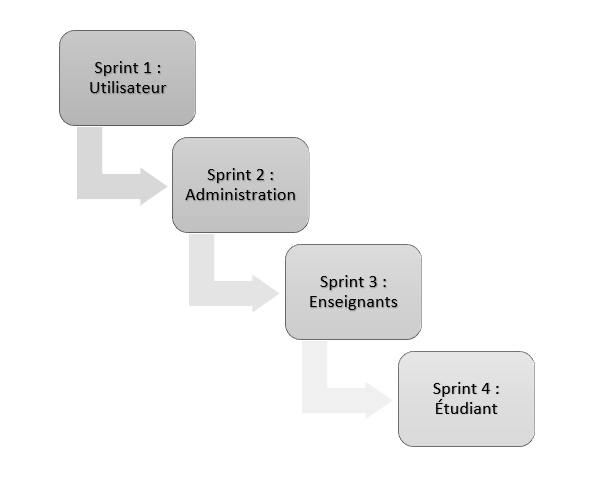
\includegraphics[width=10cm,height=8cm]{Sanstfjitre.png}
	\caption{Section de chapitre 3.}
	\label{fig:Section de chapitre 3}
\end{figure}
\FloatBarrier
\clearpage
\section{Présentation l'interfaces :page d'accueil}
Après les phases d’étude de l’existant, la conception et la modélisation fonctionnelle et
organisationnelle on a développé les interfaces de l’application.\\
La page accueil présente la page d’accueil de l’application, à partir de cette interface, si
l’internaute est un nouvel utilisateur, le site lui propose de rejoindre la communauté, donc de
créer son compte.\\
Les interfaces du site sont présentées sous forme de lien. Elles présentent cinq liens
principaux se différenciant selon l’utilisateur qu’il soit connecté ou non. \\
{\color{cyan} Lorsque l’utilisateur n’est pas connecté  :
}

\begin{itemize}
	\item \underline{Accueil }  : qui amène l’utilisateur à la page d’accueil du site .
	\item \underline{Inscription }  : qui amène l’utilisateur vers la page d’inscription.
	\item \underline{Connexion}  :qui amène l’utilisateur sur la page de connexion du site.
	
	\item \underline{la liste des catégories}  : représente la liste des catégories.
	\item \underline{meilleur cours}  :représente la liste des meilleurs cours.
\end{itemize}

\begin{figure}[ht]
	\centering
	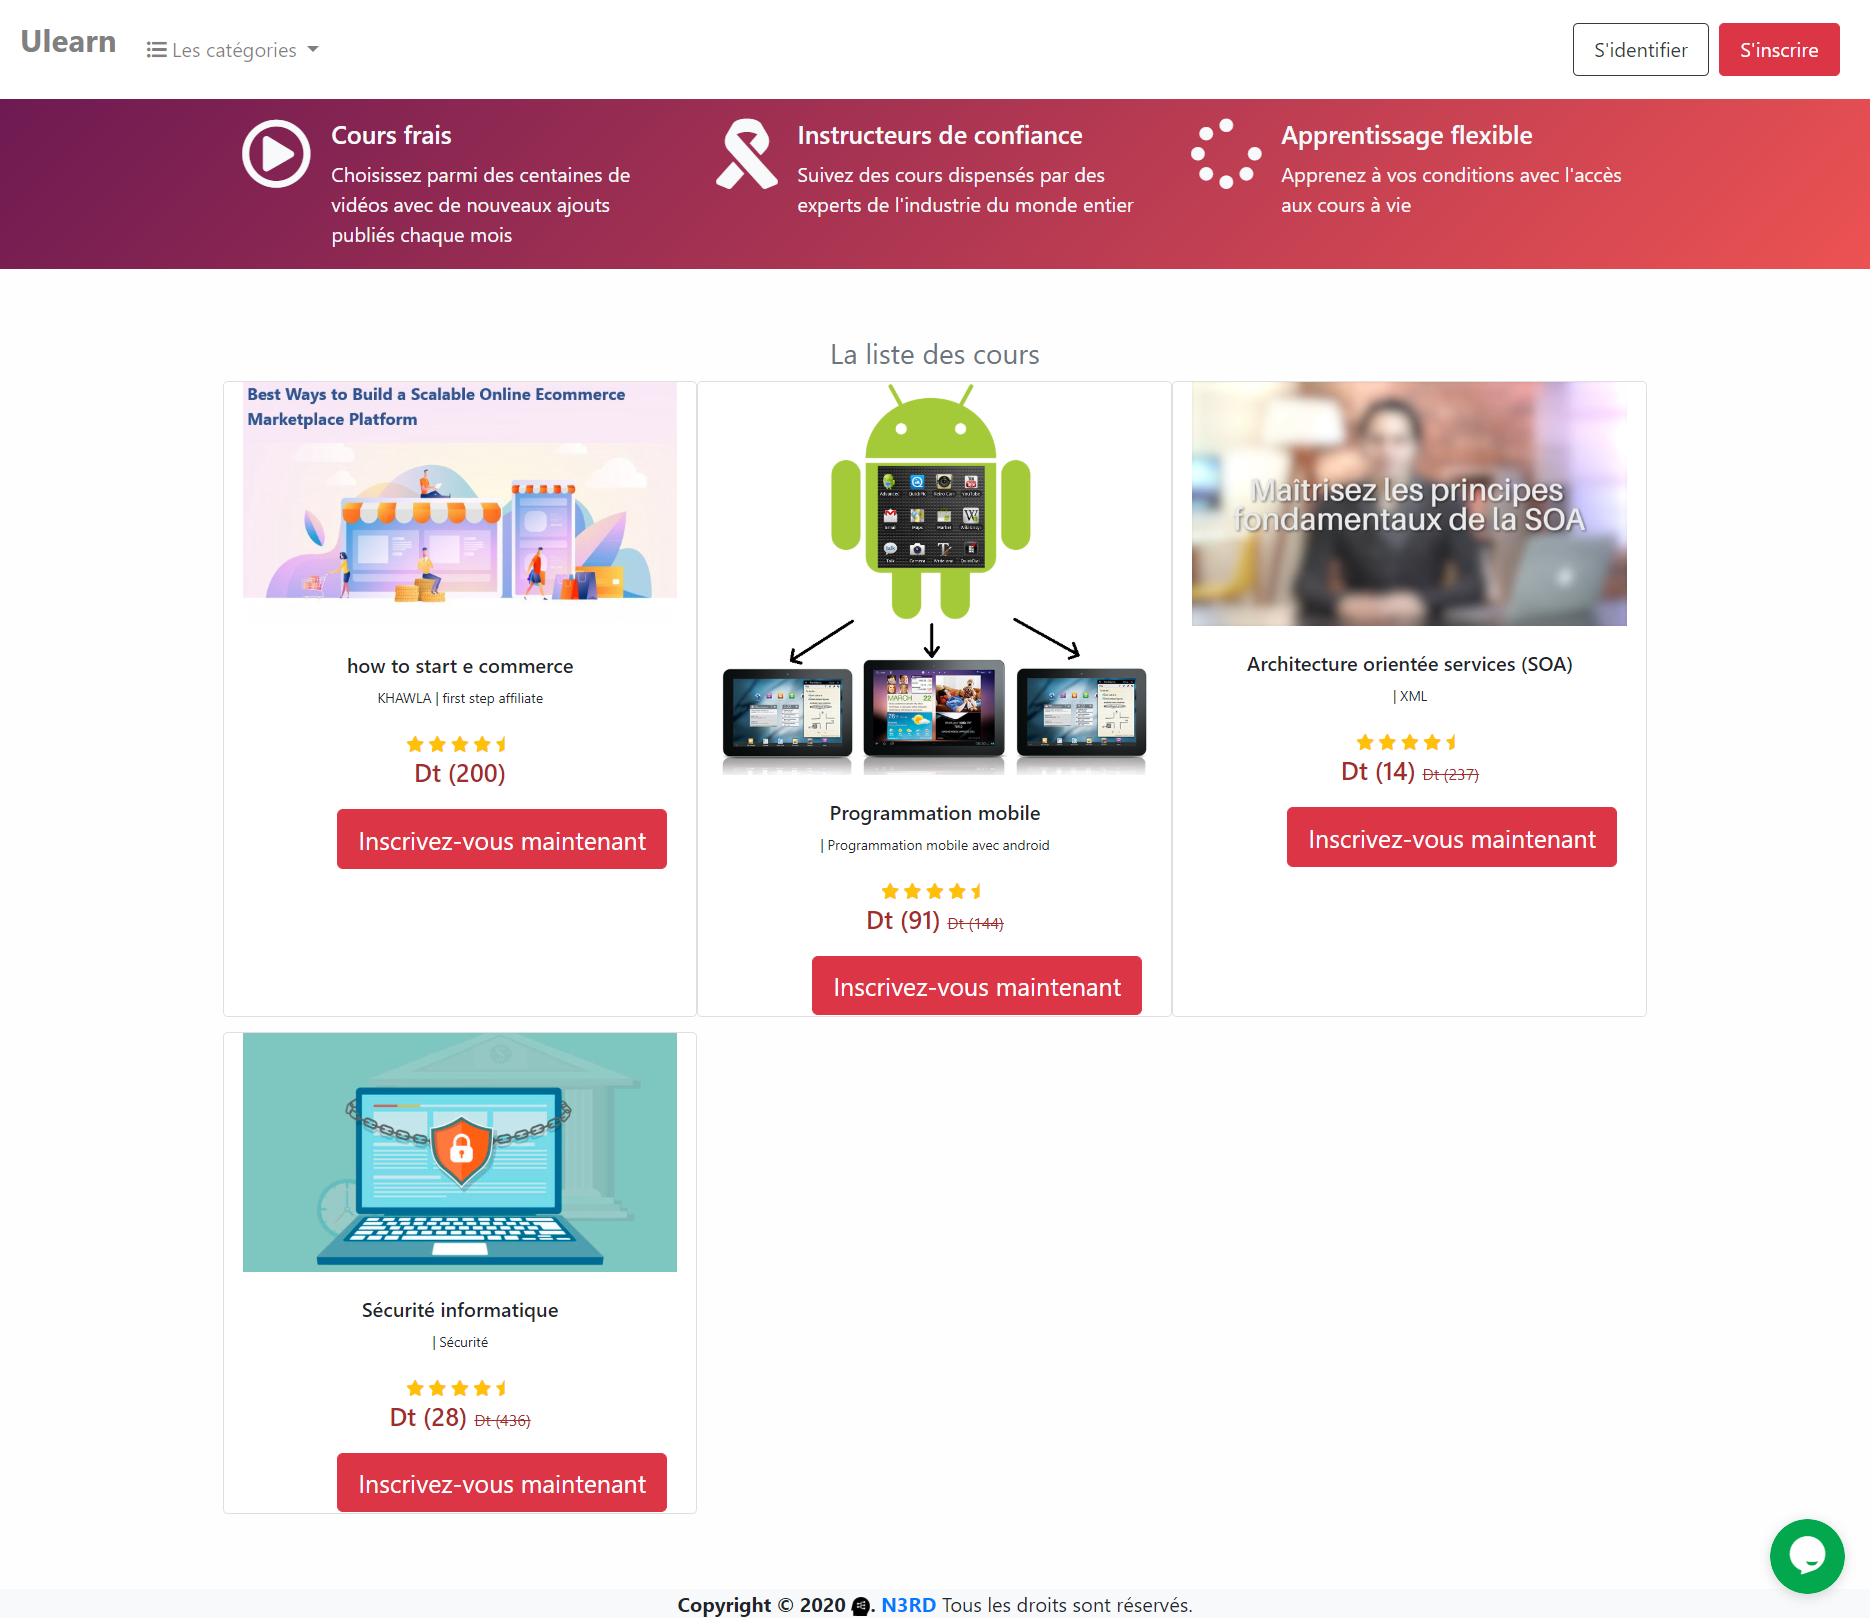
\includegraphics[width=16cm,height=9cm]{pageacui.png}
	\caption{page d'accueil.}
	\label{fig:page d'accueil }
\end{figure}
\FloatBarrier
\clearpage 
\section{Sprint 1 : Utilisateur }
\label{sec:conception}

\begin{fquote}
Ce premier sprint s’étale sur 6 jours et se décompose en 2 items  \end{fquote}
\smallskip
\begin{itemize}[label=$\diamond$]
	\item Authentification , Inscrire
	\item Gérer le profil
\end{itemize}
\medskip
\medskip
\medskip
\medskip
\medskip
\medskip
\medskip
\medskip
\medskip
\medskip
\begin{figure}[ht]
	\centering
	\includegraphics[width=13cm,height=10cm]{Décompositionsprint1enItems.png}
	\caption{Décomposition sprint 1 en Items.}
	\label{fig:Décomposition sprint 1 en Items}
\end{figure}
\FloatBarrier
\clearpage

\begin{table}[]
	{\Large \color{cyan} Le backlog du sprint 1 est le suivant :}\\
	
	\begin{tabular}{|l|l|l|l|}
		\hline 
		\rowcolor{-blue!20!red}{Item}           & \textbf{User Story}                                                   & \textbf{Description}                                                                                               & \textbf{Priorité} \\ \hline
		\textbf{s'authentifier}                    & s'authentifier                                                            &  je dois m'identifier 
		pour acceder a mon espace                                                                       & 1    \\ \hline
		
		\multirow{4}{*}{\textbf{gérer profil}} & \begin{tabular}[c]{@{}l@{}}Consulter\\ profil\end{tabular}            & \begin{tabular}[c]{@{}l@{}}En tant qu'utilisateur je peux consulter mon \\ profil\end{tabular}                    & 3                 \\ \cline{2-4} 
		& Modifier profil                                                       & \begin{tabular}[c]{@{}l@{}}En tant qu'utilisateur je peux modifier mon \\ profil\end{tabular}                     &                   \\ \cline{2-4} 
		& \begin{tabular}[c]{@{}l@{}}Modifier\\ image de \\ profil\end{tabular} & \begin{tabular}[c]{@{}l@{}}En tant qu'utilisatuer je peux uploader modifier\\ une image de profil\end{tabular}    &                   \\ \cline{2-4} 
		& Désactiver profil                                                     & \begin{tabular}[c]{@{}l@{}}En tant qu'utilisateur je peux désactiver mon\\ profil\end{tabular}                    &                   \\ \hline
		
		\textbf{s'inscrire}                    & s'inscrire                                                            & En tant qu'utilisateur, je peux m'inscrire                                                                        & 1    \\ \hline
	\end{tabular}
	
	
	\caption{Tables Backlog du sprint 1}
	\label{Tables Backlog du sprint 1}
\end{table}
% \section{end_tableau}

\begin{table}[h]
	{\Large \color{cyan} les user stories de sprint 1:}\\
	
	\begin{center}
		\begin{tabular}{>{\begin{bf} } c <{\end{bf}}ccc}
			
			\rowcolor{-blue!20!red}ID U.S & \begin{bf}User Story \end{bf}  & \\
			
			
			1.1  & En tant qu’utilisateur, je dois m’authentifier pour accéder à mon espace \\& \\
			1.2  & En tant qu’utilisateur, je peux m’inscrire \\& \\
			2.1 & En tant qu’utilisateur je peux uploader une image de profil \\& \\
			2.2  & En tant qu’utilisateur je peux afficher mon profil \\& \\
			2.3  & En tant qu’utilisateur je peux modifier mon profil \\& \\
			2.4 & En tant qu’utilisateur je peux désactiver mon profil \\
			
			
		\end{tabular}
	\end{center}
	\caption{Tables  "les user stories de sprint 1"}
	\label{les user stories de sprint 1}
\end{table}
		

\clearpage

\subsection{item 1 : Authentification}
\subsubsection{Diagramme de cas d’utilisation }

La figure \ref{fig:Diagramme de Cas d utilisation S' authentifier } ci-dessous, décrit Diagramme de Cas d' utilisation S' authentifier
de Uleran.
\begin{figure}[ht]
	\centering
	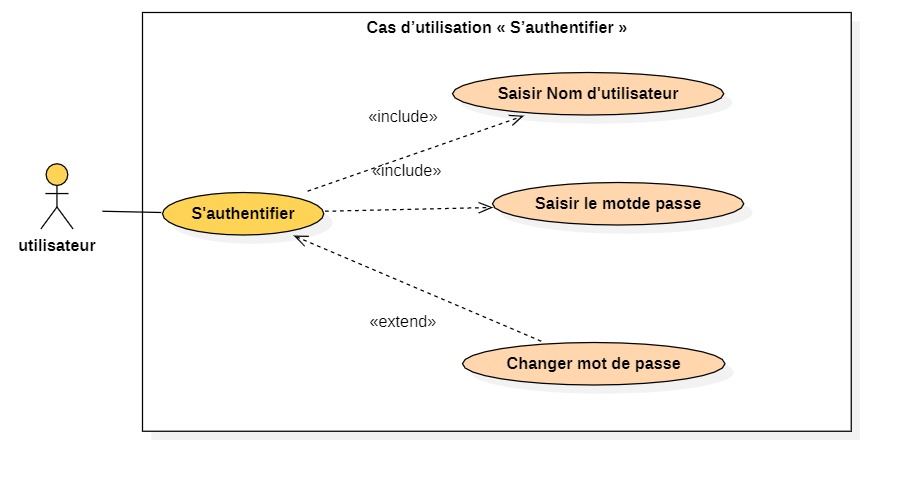
\includegraphics[width=13cm,height=10cm]{DiagrammedeCasdutilisationSauthentifier.png}
	\caption{Diagramme de Cas d' utilisation S' authentifier .}
\label{fig:Diagramme de Cas d utilisation S' authentifier }
\end{figure}
\FloatBarrier



{\Large \color{cyan} Description détaillée:}


\begin{itemize}
	
	\item[$\bullet$] \textbf{Cas d’utilisation S’authentifier :} permet aux utilisateurs de se connecter au système avec leurs logins et mots de passe afin de sécuriser la platforme.
	\medskip
	\begin{itemize}
		\item \textit{\textbf{Objectif :}}  Cette fonctionnalité permet aux différents acteurs de se connecter. 
		
		\item \textit{\textbf{Acteur :}} Tous les acteurs
		
		\item \textit{\textbf{Pré-condition  :}} L’utilisateur existe dans la base de données.
		\item \textit{\textbf{Post-conditions   :}} Utilisateur authentifié.
		\item \textit{\textbf{Scénario nominal :}}
		\begin{enumerate}
			\item L’acteur saisit son login et son mot de passe. 
			\item Le système vérifie les informations saisies. 
			\item Le système trouve que les informations saisies sont valides.  
			\item Le système vérifie le rôle de l’acteur.  
			\item Le système connecte l’acteur à son espace.
		\end{enumerate}
		\item \textit{\textbf{Scénario d'erreur :}} 
		\begin{enumerate}
			\item L’acteur saisit son login et son mot de passe. 
			\item Le système vérifie les informations saisies.   
			\item Le système trouve que les informations saisies sont invalides.  
			\item Le système demande à l’acteur de vérifier les informations saisies.
		\end{enumerate}
	\end{itemize}	
	\bigskip
\end{itemize}
\bigskip
\subsubsection{Diagrammes de séquence système }

\begin{figure}[ht]
	\centering
	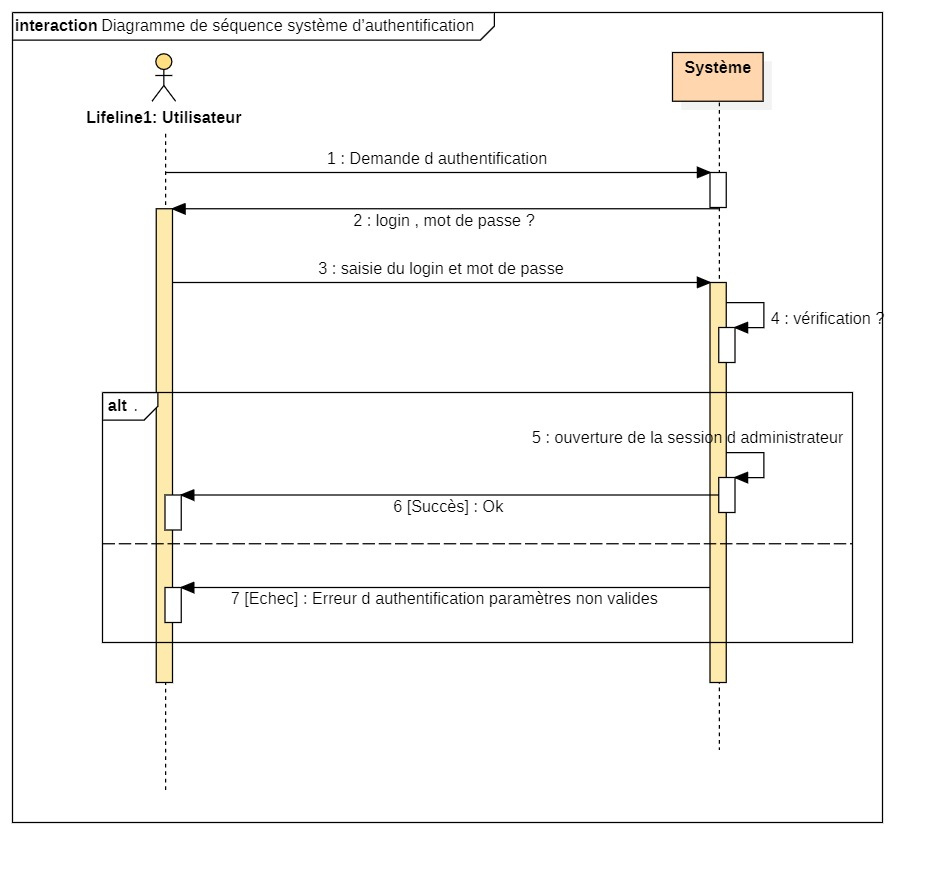
\includegraphics[width=13cm,height=10cm]{Diagrséquencesystèmeauthentification.jpg}
	\caption{Diagramme de séquence système d' authentification .}
	\label{fig:Diagramme de séquence système d' authentification }
\end{figure}
\FloatBarrier
Pour s’authentifier, un administrateur doit saisir son login et son mot de passe, si les
données saisies sont correctes alors sa session sera ouverte et il sera redirigé automatiquement au dashboard dela plateforme. Si les données sont erronées alors un message d’erreur
apparaîtra lui demandant de saisir de nouveau le login et le mot de passe corrects.
\clearpage
\subsubsection{les Interfaces : Authentification  }


\begin{figure}[ht]
	\centering
	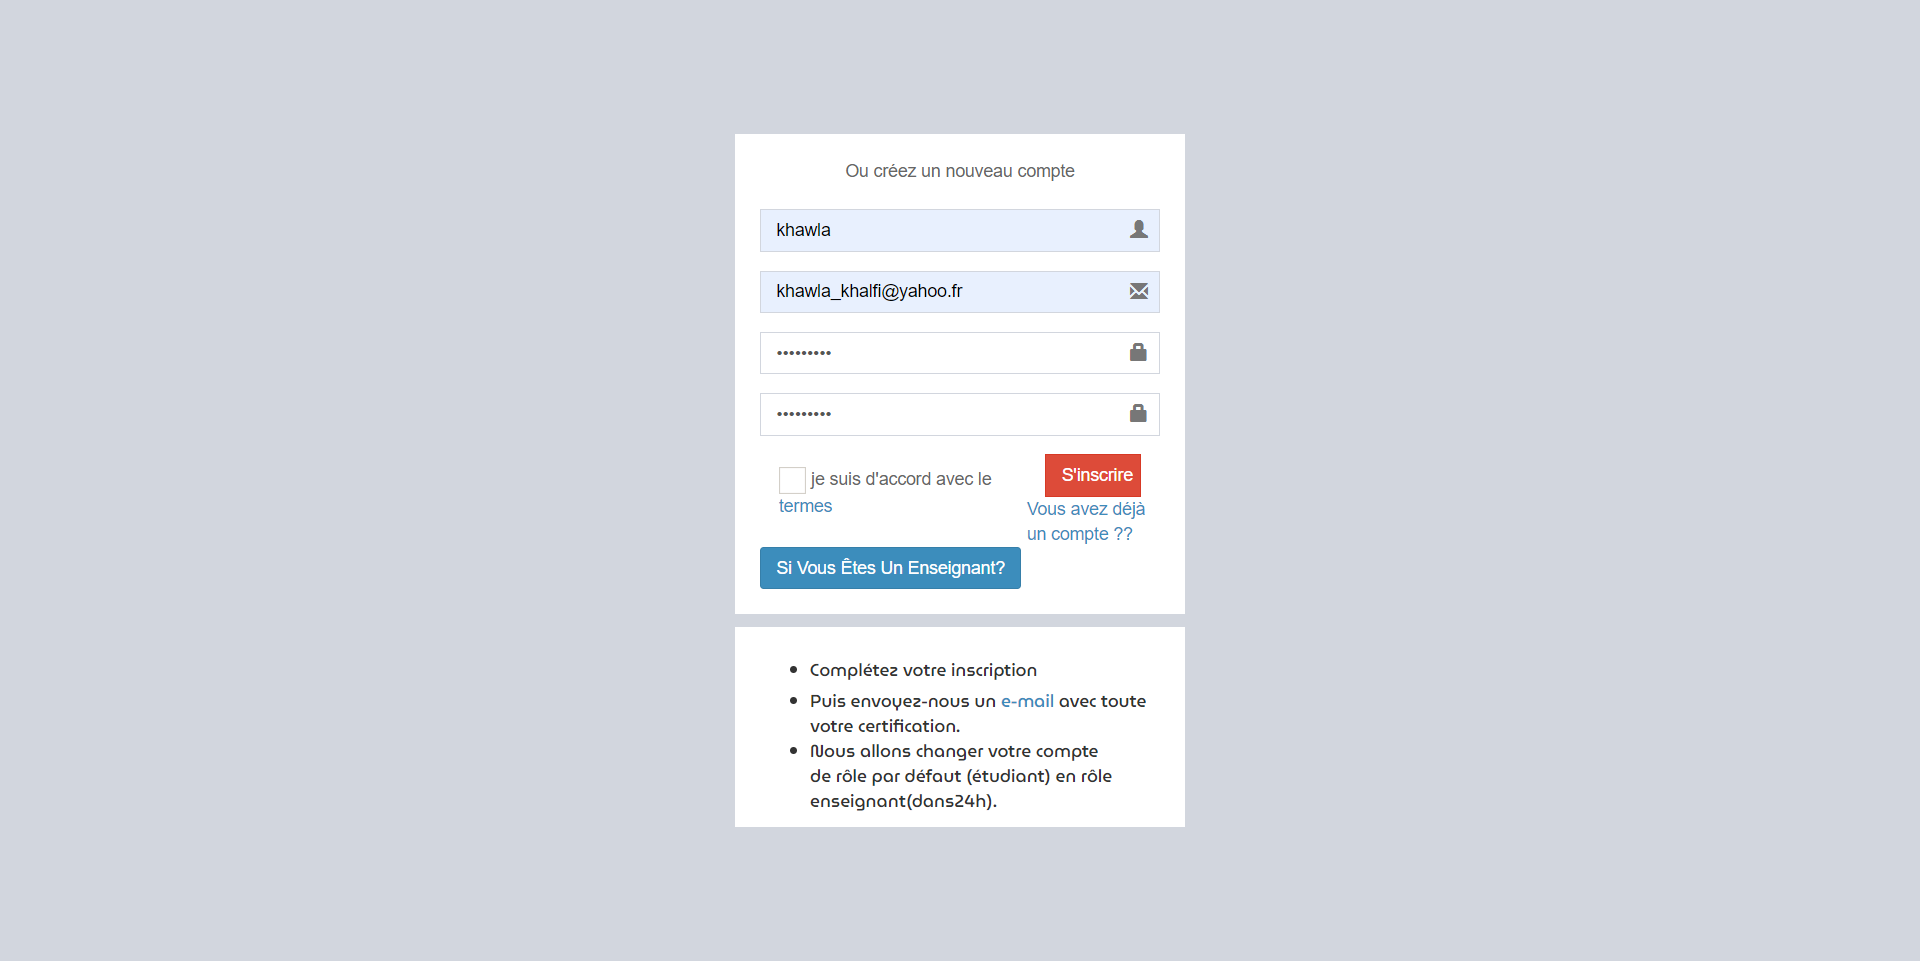
\includegraphics[width=10cm,height=6.2cm]{inscription.png}
	\caption{Interface : Inscription .}
	\label{fig:Interface : inscription }
\end{figure}
\FloatBarrier
Un nouveau utilisateur doit créer un compte, pour s’inscrire il remplit le formulaire et
choisit un mot de passe. 


\begin{figure}[ht]
	\centering
	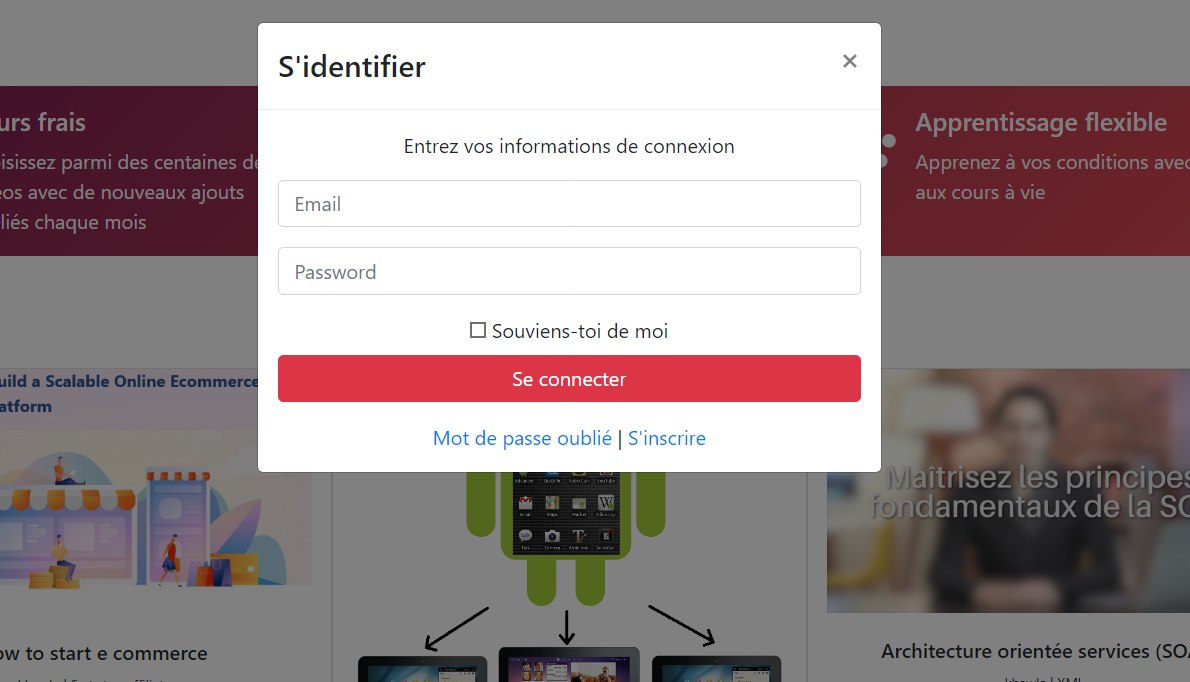
\includegraphics[width=17cm,height=8cm]{identif.png}
	\caption{Interface : Authentification .}
	\label{fig:Interface : Authentification }
\end{figure}
\FloatBarrier
Si les coordonnés de l’utilisateur sont erronées, le système affiche un message d’erreur et
l’invite à ressaisir ses coordonnés.
Sinon l’utilisateur est redirigé vers sa page d’accueil, dans lequel on trouve un menu de tous les
modules de l’application et chacun de ces modules contient un ensemble des fonctionnalités
sous forme des sous menus relatifs à ce module.
\clearpage
\subsection{item 2 : Gérer le profil}
\subsubsection{Diagramme de cas d’utilisation }


\begin{figure}[ht]
	\centering
	\includegraphics[width=13cm,height=10cm]{CasutilisationGérprofil.jpg}
	\caption{Diagramme de Cas d' utilisation Gérer le profil .}
	\label{fig:Gérer le profil }
\end{figure}
\FloatBarrier

{\Large \color{cyan} Description détaillée:}
\begin{itemize}
	
	\item[$\bullet$] \textbf{Cas d’utilisation Gérer le profil :} permet à l’acteur de mettre à jour ses informations.
	\medskip
	\begin{itemize}
		\item \textit{\textbf{Objectif :}}  Cette fonctionnalité permet aux différents acteurs de mettre à jour ses informations. 
		
		\item \textit{\textbf{Acteur :}} Tous les acteurs
		
		\item \textit{\textbf{Pré-condition  :}}  L‘acteur doit être un membre identifié.
		\item \textit{\textbf{Post-conditions   :}} le cas démarre après le point 02 de l’enchainement nominal.
		\item \textit{\textbf{Scénario nominal :}}
		\begin{enumerate}
			\item le système affiche le profil actuel de l’acteur. 
			\item l’acteur met à jour ses informations. 
			\item  le système vérifie la validité des informations saisies.  
			\item  le système enregistre ces informations dans la base de données .  
			\item le système notifie l’acteur du bon déroulement de mise à jour de son profil
		\end{enumerate}
		\item \textit{\textbf{Scénario alternative :}} \\
			les informations sont manquantes ou incorrectes: ce scénario commence au point 03 du
		scénario nominal.
		\begin{enumerate}
		
			\item Le système informe l’acteur que les données saisies sont erronées, garde les informations
			saisies avant et le scénario reprend au point 02 du scénario nominal. 
		\end{enumerate}
	\end{itemize}
\end{itemize}	
	\bigskip


\subsubsection{ Interface : Gérer le profil  }


\begin{figure}[ht]
	\centering
	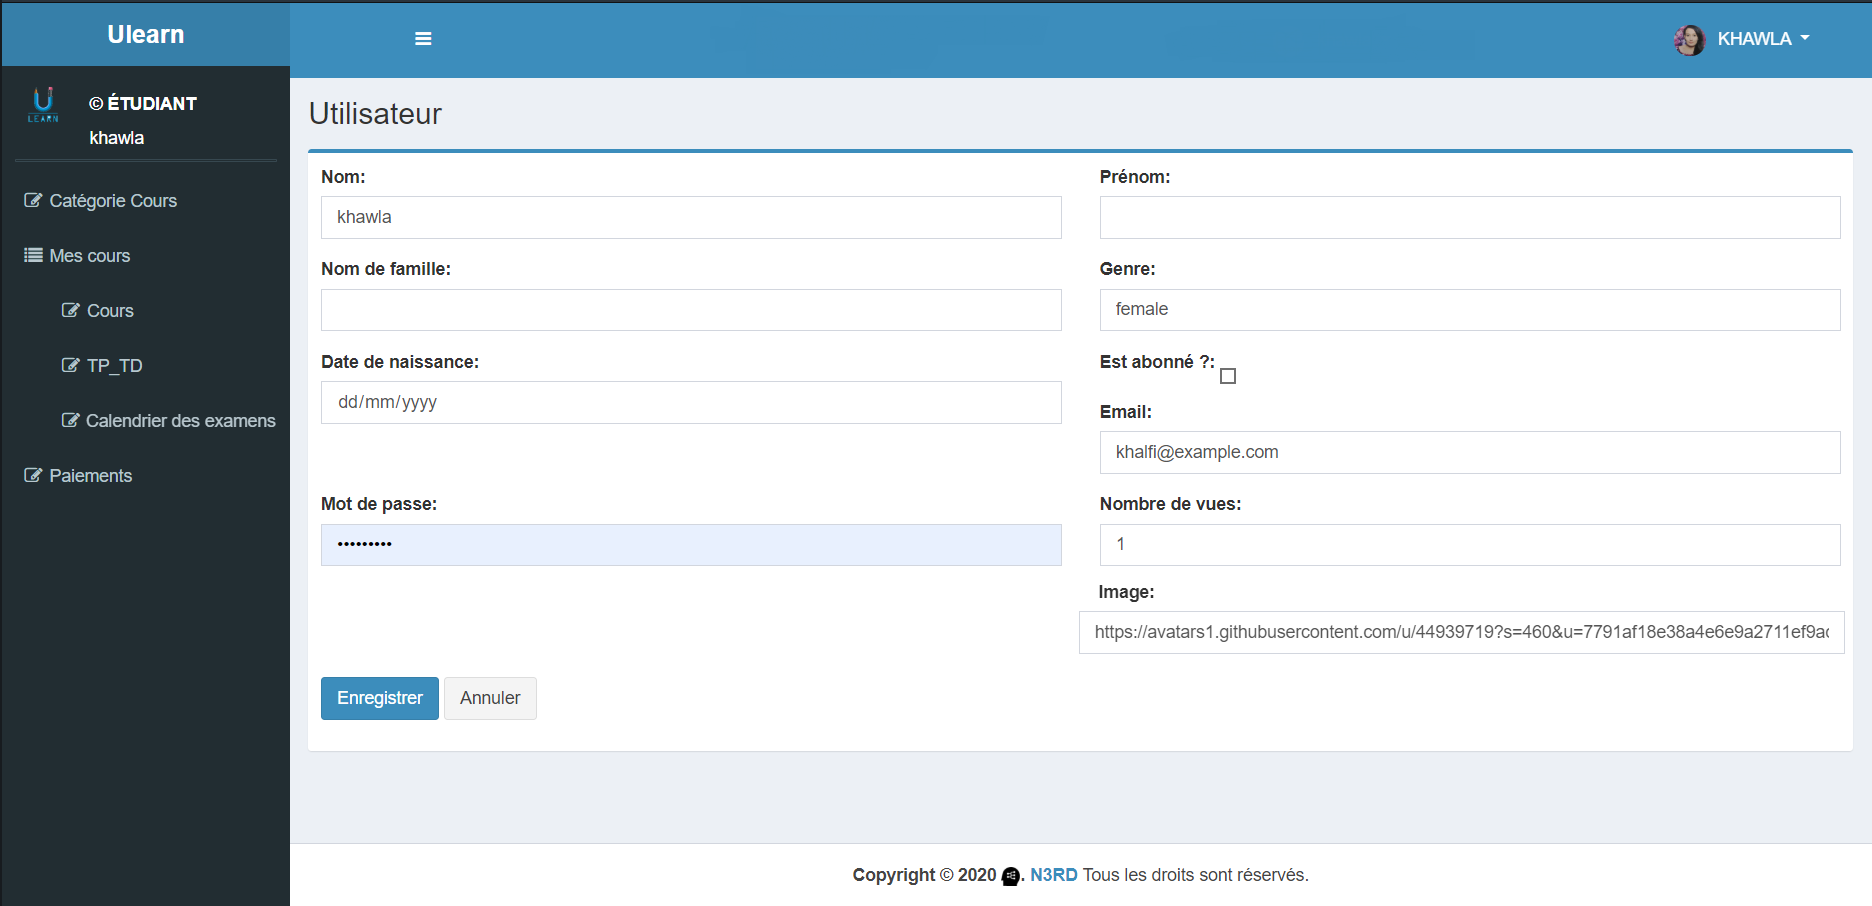
\includegraphics[width=17cm,height=11cm]{editprofparetud.png}
	\caption{Interface : Gérer le profil .}
	\label{fig:Interface : Gérer le profi }
\end{figure}
\FloatBarrier
Après activation de son compte. L’utilisateur peut maintenant se connecter pour ouvrir sa session.
Lorsque ses informations de connexion sont validées, l’utilisateur sera redirigé vers
l’interface de son profil avec l’avatar par défaut et aucune formation pour le moment (il peut modifier son profile) .


\clearpage



\section{Sprint 2 : Administration }



\begin{fquote}
Ce premier sprint s’étale sur 10 jours et se décompose en 3 items \end{fquote}
\smallskip
\begin{itemize}[label=$\diamond$]
	\item Gérer les utilisateurs
    \item  vérifier les conditions d'inscription pour les utilisateurs
    \item  Gestion des rôles utilisateurs
	
\end{itemize}
\medskip
\medskip
\medskip
\medskip
\medskip
\medskip
\medskip
\medskip
\medskip
\medskip
\medskip
\begin{figure}[ht]
	\centering
	\includegraphics[width=13cm,height=10cm]{Décompositionsprint2enItems.png}
	\caption{Décomposition sprint 2 en Items.}
	\label{fig:Décomposition sprint 2 en Items}
\end{figure}
\FloatBarrier
\clearpage


   
 



\begin{table}[]
	{\Large\color{cyan} Le backlog du sprint 2 est le suivant :}\\
	
	\begin{tabular}{|l|l|l|l|}
		\hline 
		\rowcolor{-blue!20!red}{Item}                         & \textbf{User Story}                                                   & \textbf{Description}                                                                                              & \textbf{Priorité} \\ \hline
		\begin{tabular}[c]{@{}l@{}}\textbf{ vérifier }\\ \textbf{ les conditions }\\ \textbf{d'inscription pour  }\\ \textbf{les utilisateurs  } \end{tabular}                & \begin{tabular}[c]{@{}l@{}} vérifier les conditions\\ d'inscription pour\\ les utilisateurs \end{tabular}                                                         & \begin{tabular}[c]{@{}l@{}}en tant que je suis\\ l'administrateur je peux vérifier \\les conditions d'inscription utilisateur\\ si l'utilisateur est un enseignant \\il faut me envoyer \\ leur CV pour Candidat au poste  .\end{tabular} & 2               \\ \hline
		\multirow{4}{*}{\begin{tabular}[c]{@{}l@{}}\textbf{Gérer  }\\ \textbf{les utilisateurs  } \end{tabular}}
		
		
		
		
		
		
		
		& \begin{tabular}[c]{@{}l@{}}Gérer les\\  utilisateurs \\ \end{tabular}       & \begin{tabular}[c]{@{}l@{}}En tant que je suis un administrateur\\ je peux gérer les utilisateurs :\\je peux ajouter des utilisateurs \\  comme des enseignants je peux\\ supprimer des utilisateurs\\ comme des étudiants et je peux \\modifier comme changer \\le rôle ou bien mise à jour\\ ces informations .\end{tabular}                    & 1                              
		\\ \hline
		
		\begin{tabular}[c]{@{}l@{}}\textbf{gère les  }\\ \textbf{ rôles  } \\ \textbf{ utilisateurs}\end{tabular}                   & \begin{tabular}[c]{@{}l@{}}gère les  \\  rôles \\ des utilisateurs   \end{tabular}                                                           & \begin{tabular}[c]{@{}l@{}}	en tant que je suis un\\ administrateur je peux ajouter \\ des nouveaux rôle et aussi \\je peux changer le rôle d'un utilisateur \end{tabular}                                    & 3    \\ \hline
	\end{tabular}
	
	
	\caption{Tables Backlog du sprint 2}
	\label{Tables Backlog du sprint 2}
\end{table}


\begin{table}[h]
	{\Large\color{cyan} les user stories de sprint 2:}\\
	
	\begin{center}
		\begin{tabular}{>{\begin{bf} } c <{\end{bf}}ccc}
			
			\rowcolor{-blue!20!red}ID U.S & \begin{bf}User Story \end{bf}  & \\
			
			1 &en tant que je suis un administrateur \\
			&je peux accéder à l'interface d'ajout \\
			&utilisateur  où je peux supprimer ,\\
			& modifier  ce utilisateur .    
			
			& \\	2 &s'il confirme toutes les conditions de vérifications \\ 
			&de son statut (enseignant), l'administration acceptera sa \\ 
			&demande de changer le rôle de son compte en\\ 
			& rôle d'enseignant
			\\
			3 & en tant que je suis un administrateur \\ 
			& je peux changer les rôles des  utilisateurs
			\\
			
			
			
			
		\end{tabular}
	\end{center}
	\caption{Tables  "les user stories de sprint 2"}
	\label{les user stories de sprint 2}
\end{table}




\clearpage

%{+++++++++++++++++un autre section+++++++++++++++++++ }
%{+++++++++++++++++un autre section+++++++++++++++++++ }
%{+++++++++++++++++un autre section+++++++++++++++++++ }
%{+++++++++++++++++un autre section+++++++++++++++++++ }
 
\subsection{item 1 : Gérer les utilisateurs}
\subsubsection{Diagramme de cas d’utilisation  détaillé «administrer du plateforme» }

\begin{figure}[ht]
	\centering
	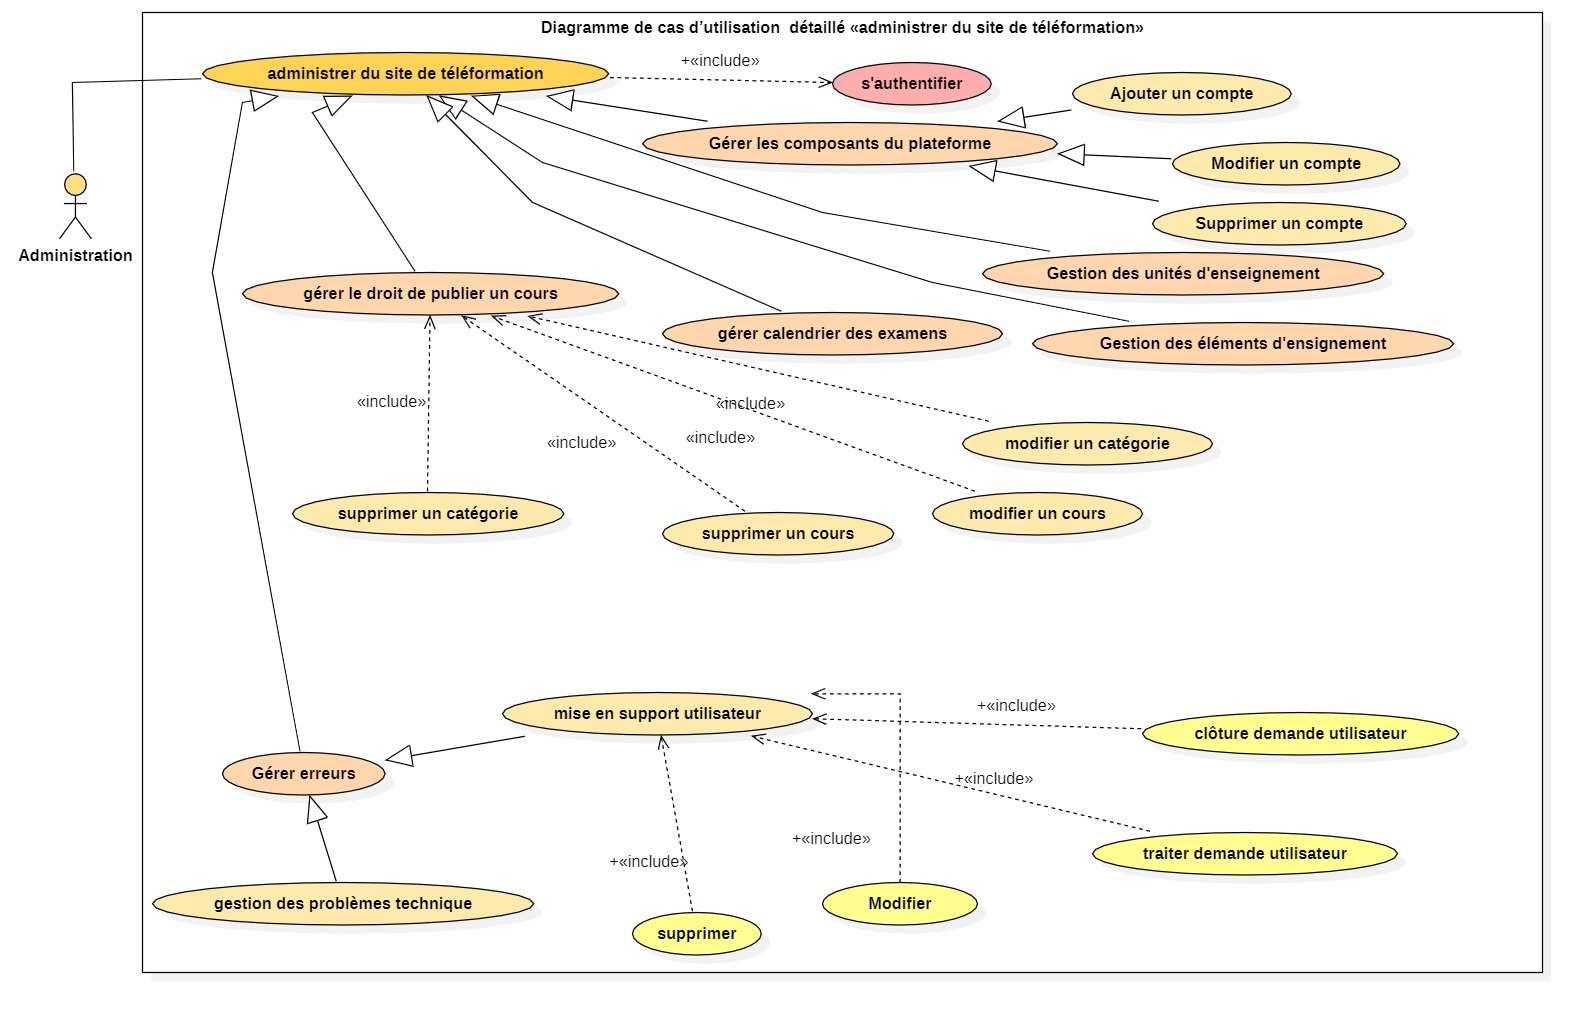
\includegraphics[width=18cm,height=16cm]{Diagrammedecasdutilisationdétailléadministr.jpg}
	\caption{Diagramme de cas d' utilisation  détaillé «administrer» .}
	\label{fig:Diagramme de cas d' utilisation  détaillé administrer  }
\end{figure}
\FloatBarrier
\clearpage
%{+++++++++++++++++un autre section+++++++++++++++++++ }
%{+++++++++++++++++un autre section+++++++++++++++++++ }
%{+++++++++++++++++un autre section+++++++++++++++++++ }
%{+++++++++++++++++un autre section+++++++++++++++++++ }
{\Large \color{cyan} Description détaillée des cas d’utilisations : gérer les composants de plate-forme}

L'administrateur a comme rôle principale de gérer toutes les taches de la plateforme; gestion des enseignants, étudiants ,matières....ainsi que les affectations des
enseignants.\\
L'administrateur peut ajouter, supprimer ou modifier les différentes informations des étudiants d'une manière permanente.\\
L'administrateur peux dérer des droits et des erreures et il donne le droit à l'enseignant pour publier leur cours après  consulat  de leur contenu .
\begin{itemize}
      \item[$\bullet$] \textbf{Cas d’utilisation Gérer le profil :} permet à l’acteur de mettre à jour la plateforme. 
	\medskip
	\begin{itemize}
		\item \textit{\textbf{Objectif :}}  permet à l’administrateur de modifier la composition interne de la plateforme. 
		
		\item \textit{\textbf{Acteur :}} Administrateur
		
		\item \textit{\textbf{Pré-condition  :}}  L‘acteur doit être connecté.
		\item \textit{\textbf{Post-conditions   :}}
		\item \textit{\textbf{Scénario nominal :}}
		\begin{enumerate}
			\item le système affiche l’état actuel de la plateforme. 
			\item l’acteur met à jour la plateforme. 
			\item   le système vérifie la validité des mis à jour.  
			\item  le système enregistre les mis à jours dans la base de données.  
			\item le système notifie l’acteur du bon déroulement de mise à jour de la plateforme.
		\end{enumerate}
		\item \textit{\textbf{Scénario alternative :}} \\
les informations sont manquantes ou incorrectes: ce scénario commence au point 03 du
scénario nominal
		\begin{enumerate}
			\item  Le système informe l’acteur que les mis à jour sont erronées, garde l’état de la plateforme 
		\end{enumerate}
	\end{itemize}
\end{itemize}
\clearpage	
%{+++++++++++++++++un autre section+++++++++++++++++++ }
%{+++++++++++++++++un autre section+++++++++++++++++++ }
%{+++++++++++++++++un autre section+++++++++++++++++++ }
%{+++++++++++++++++un autre section+++++++++++++++++++ }
\subsubsection{Diagrammes de séquence du cas d' utilisation "Modifier un utilisateur" }
\begin{figure}[ht]
	\centering
	\includegraphics[width=14cm,height=13cm]{DiagrammesdeséquenceducasdutilisationModifierunutilisa.jpg}
	\caption{Diagrammes de séquence du cas d' utilisation "Modifier un utilisateur"  .}
	\label{fig:Diagrammes de séquence du cas d' utilisation Modifier un utilisateur }
\end{figure}
\FloatBarrier

{\Large \color{cyan} Description détaillée: "Modifier un utilisateur"}
\begin{itemize}
	\item[$\bullet$] \textbf{Cas d’utilisation "Modifier un utilisateur" :} 
	\medskip
	\begin{itemize}
		\item \textit{\textbf{Objectif :}} Modifier un utilisateur 	
		\item \textit{\textbf{Acteur :}} Administrateur	
		\item \textit{\textbf{Pré-condition  :}} Authentification préalable.\\
		Utilisateur existant.\\
		Formulaire d’ajout disponible.
\\
		\item \textit{\textbf{Post-conditions   :}}L’utilisateur a bien été modifié .
		\item \textit{\textbf{Scénario nominal :}}
		\begin{enumerate}
			\item L’utilisateur demande le formulaire de modification d’un utilisateur.
			\item Le système affiche le formulaire avec l’ensemble des anciennes informations de l’utilisateur.
			\item L’administrateur modifie les champs nécessaires. 
			\item Le système vérifie les données saisies. 
			\item L’administrateur valide la modification . 
			\item Le système vérifie l’existence de l’utilisateur .  
			\item Le système modifie l’utilisateur.
		\end{enumerate}
		\item \textit{\textbf{Scénario alternative :}}
		\begin{enumerate}
			\item L’utilisateur saisit des informations manquantes ou erronées.
			\item  Le système renvoie un message d’erreur adéquat.
			\item Reprise de l’étape 3 du scénario Nominal.
		\end{enumerate}
	\end{itemize}
\end{itemize}	
%{+++++++++++++++++un autre section+++++++++++++++++++ }
%{+++++++++++++++++un autre section+++++++++++++++++++ }
%{+++++++++++++++++un autre section+++++++++++++++++++ }
%{+++++++++++++++++un autre section+++++++++++++++++++ }

\subsubsection{Diagramme de séquence du cas d' utilisation "Supprimer un utilisateur" }
\begin{figure}[ht]
	\centering
	\includegraphics[width=14cm,height=10cm]{DiagrammedeséquenceducasdutilisationSupprimerunutilisateur.jpg}
	\caption{ Diagramme de séquence du cas d' utilisation "Supprimer un utilisateur"  .}
	\label{fig: Diagramme de séquence du cas d' utilisation Supprimer un utilisateur  }
\end{figure}
\FloatBarrier
\clearpage	
{\Large \color{cyan} Description détaillée: "Supprimer un utilisateur"}
\begin{itemize}
	\item[$\bullet$] \textbf{Cas d’utilisation "Supprimer un utilisateur" :} 
	\medskip
	\begin{itemize}
		\item \textit{\textbf{Objectif :}} Supprimer un utilisateur	
		\item \textit{\textbf{Acteur :}} Administrateur	
		\item \textit{\textbf{Pré-condition  :}} Authentification préalable.\\
		Utilisateur existant.
		\item \textit{\textbf{Post-conditions   :}}L’utilisateur a bien été supprimé.
		\item \textit{\textbf{Scénario nominal :}}
		\begin{enumerate}
			\item L’administrateur choisit l’utilisateur à supprimer. 
			\item Le système affiche un message de confirmation. 
			\item  L’administrateur valide son choix . 
			\item  Le système supprime l’utilisateur.  
			\item Le système affiche un message de succès.
		\end{enumerate}
		\item \textit{\textbf{Scénario alternative :}}
		\begin{enumerate}
			\item Le L’administrateur annule son choix.
			\item Le système annule la suppression.
		\end{enumerate}
	\end{itemize}
\end{itemize}
%{+++++++++++++++++un autre section+++++++++++++++++++ }
%{+++++++++++++++++un autre section+++++++++++++++++++ }
%{+++++++++++++++++un autre section+++++++++++++++++++ }
%{+++++++++++++++++un autre section+++++++++++++++++++ }
	
\subsubsection{Diagrammes de séquence du cas d' utilisation "Ajouter un utilisateur" }
\begin{figure}[ht]
	\centering
	\includegraphics[width=13cm,height=7.5cm]{DiagrammesdeséquenceducasdutilisationAjouterunutilisateur.jpg}
	\caption{Diagrammes de séquence du cas d' utilisation "Ajouter un utilisateur"  .}
	\label{fig:Diagrammes de séquence du cas d' utilisation Ajouter un utilisateur  }
\end{figure}
\FloatBarrier
\clearpage
{\Large \color{cyan} Description détaillée: "Ajouter un utilisateur"}
\begin{itemize}
	\item[$\bullet$] \textbf{Cas d’utilisation "Ajouter un utilisateur" :} 
	\medskip
	\begin{itemize}
		\item \textit{\textbf{Objectif :}} Ajouter un utilisateur pour qu’il avoir l’accés au fonctionnalités de l’espace	
		\item \textit{\textbf{Acteur :}} Administrateur	
		\item \textit{\textbf{Pré-condition  :}} Authentification préalable.\\
		Un formulaire d’ajout des utilisateurs est disponible.
		\item \textit{\textbf{Post-conditions   :}}Un nouvel utilisateur ajouté.
		\item \textit{\textbf{Scénario nominal :}}
		\begin{enumerate}
			\item L’administrateur demande un formulaire d’ajout d’un nouveau utilisateur.
			\item Le système affiche le formulaire d’ajout.
			\item L’administrateur doit remplir le formulaire avec l’ensemble des informations
			nécessaires à l’ajout du nouvel utilisateur. 
			\item Le système vérifie les données saisies. 
			\item  L’administrateur valide . 
			\item  Le système vérifie l’existence du nouveau compte .  
			\item Le système enregistre les informations saisies du l’utilisateur.
		\end{enumerate}
		\item \textit{\textbf{Scénario alternative :}}
		\begin{enumerate}
			\item L’utilisateur saisit les informations manquantes ou erronées.
			\item Le système affiche un ou des message d’erreurs selon les champs invalides.
			\item Reprise de l’étape 3 du scénario nominal.
			\item L’utilisateur existe déjà.
			\item Le système informe l’administrateur que l’utilisateur existe déjà dans le système.
			\item Reprise de l’étape 3 du scénario nominal.
		\end{enumerate}
	\end{itemize}
\end{itemize}	
\bigskip
\clearpage
%{+++++++++++++++++un autre section+++++++++++++++++++ }
%{+++++++++++++++++un autre section+++++++++++++++++++ }
%{+++++++++++++++++un autre section+++++++++++++++++++ }
%{+++++++++++++++++un autre section+++++++++++++++++++ }

\subsubsection{Diagramme d’activités « Gérer les utilisateurs » }
\begin{figure}[ht]
	\centering
	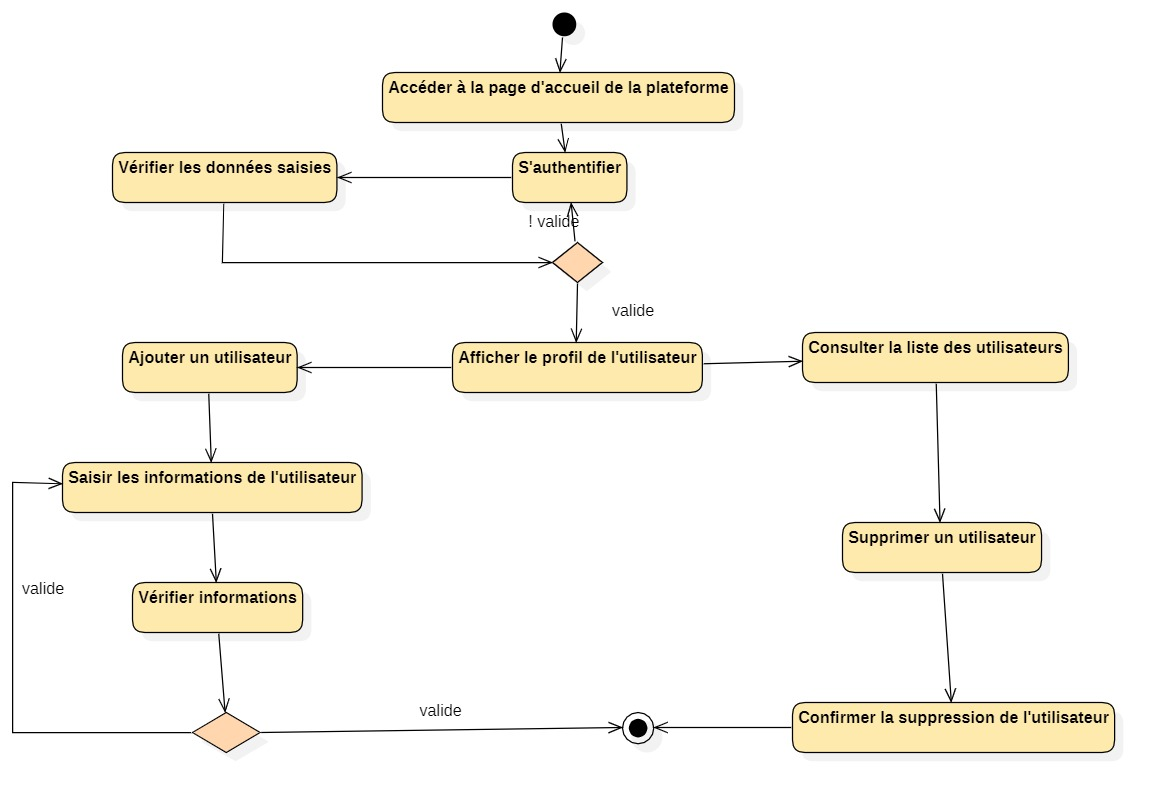
\includegraphics[width=14cm,height=14cm]{DiagrammeactivitésGérerlesutilisateurs.jpg}
	\caption{Diagramme d' activités  « Gérer les utilisateurs »  .}
	\label{fig:Diagramme d' activités  Gérer les utilisateurs  }
\end{figure}
\FloatBarrier

{\Large \color{cyan} Description détaillée:}
La figure ci-dessus illustre le déroulement séquentiel de la gestion des utilisateurs accomplis par
un administrateur .\\
Après avoir s’authentifié, ces derniers peuvent ajouter ou supprimer un utilisateur.\\
Pour l’ajout d’un utilisateur, le système doit vérifier la validation des informations saisies.\\
 Au cas où une information n’est pas valide, le système réaffiche l’interface d’ajout d’un utilisateur.
 %{+++++++++++++++++un autre section+++++++++++++++++++ }
 %{+++++++++++++++++un autre section+++++++++++++++++++ }
 %{+++++++++++++++++un autre section+++++++++++++++++++ }
 %{+++++++++++++++++un autre section+++++++++++++++++++ }
 \clearpage
 \subsubsection{ Interface : Gérer les utilisateurs   }
 Après l'authentification l'administrateur  à l'accès  de modifier , de supprimer et d'ajouter un nouvel utilisateur ,la figure ci-dessous représente le formulaire de gérer les utilisateurs.
 \begin{figure}[ht]
 	\centering
 	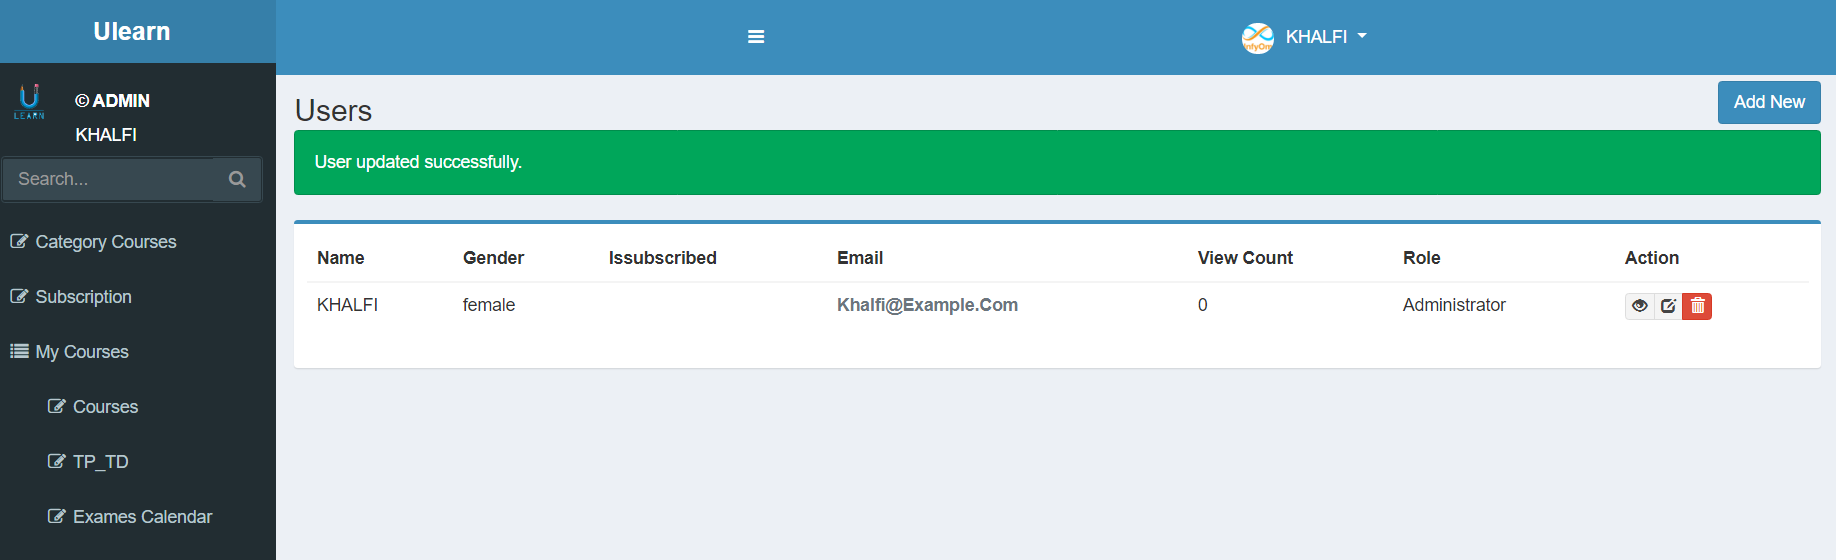
\includegraphics[width=13cm,height=6cm]{SDFI.png}
 	\caption{l'interface de gérer les utilisateurs .}
 	\label{fig:l'interface de gérer les utilisateurs    }
 \end{figure}
 \FloatBarrier
 la figure ci-dessous représente la liste des et utilisateur .
  \begin{figure}[ht]
 	\centering
 	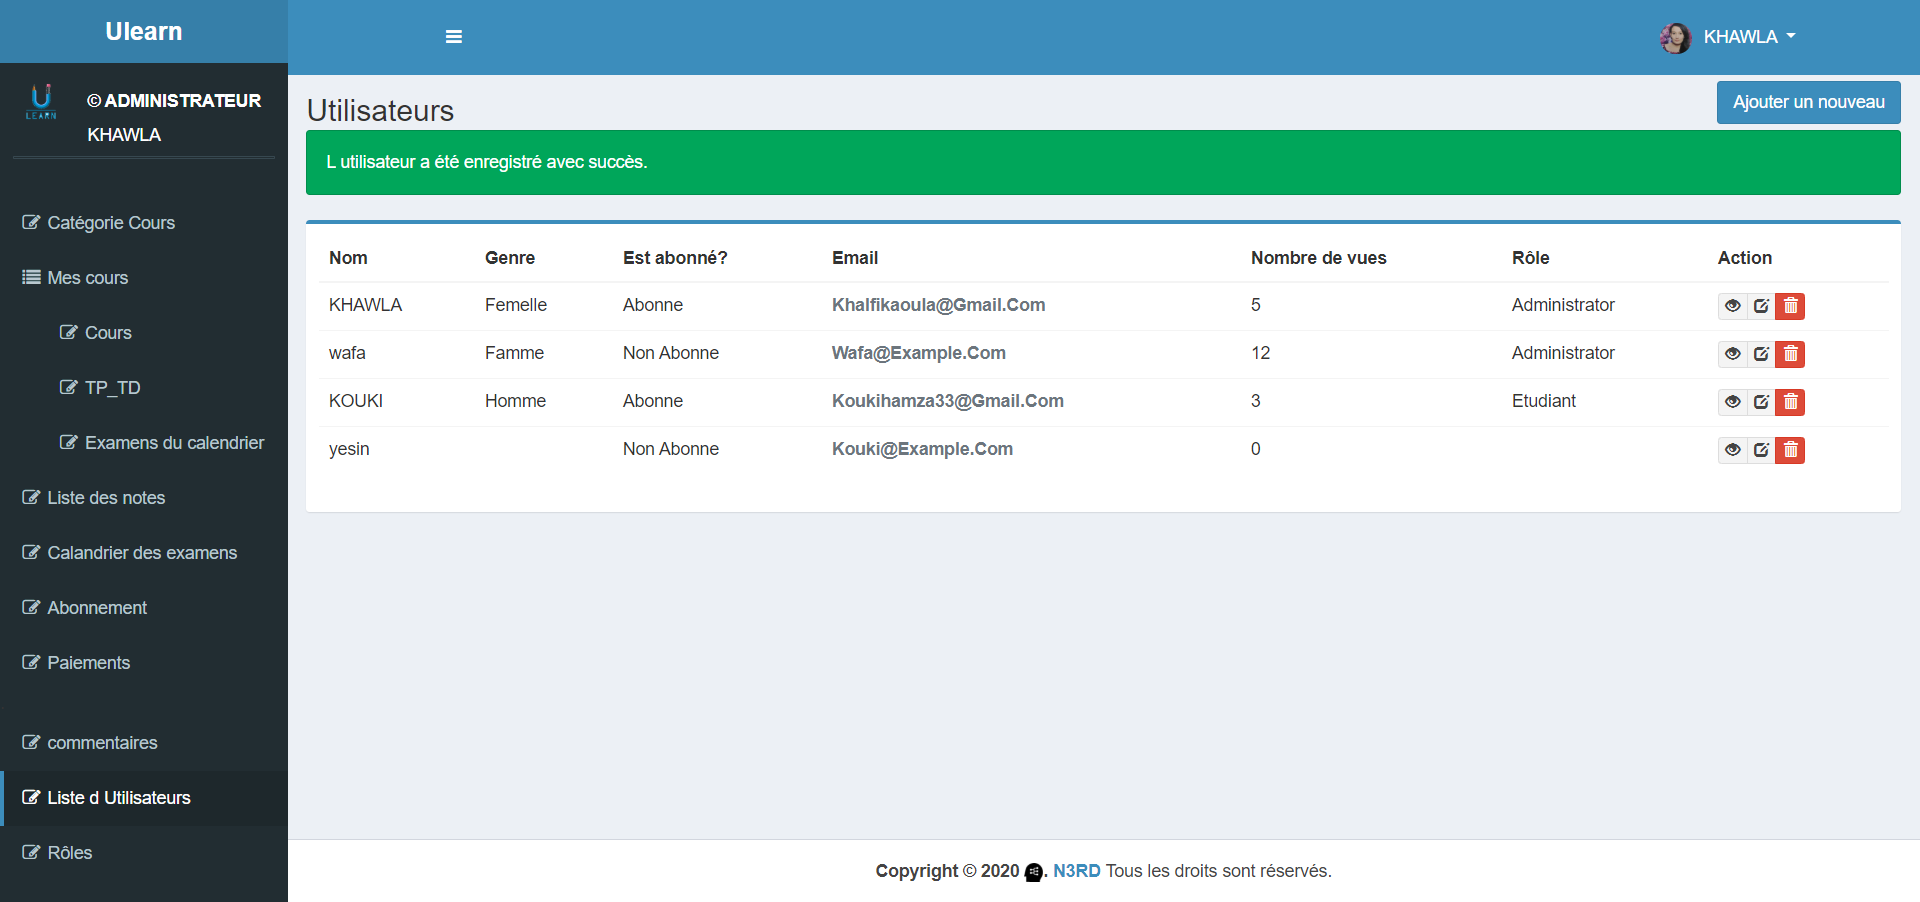
\includegraphics[width=13cm,height=6cm]{screencapture-localhost-8000-users-2020-06-24-21_01_22.png}
 	\caption{la liste des utilisateurs avec une modification .}
 	\label{fig:la liste des utilisateurs avec une modification  }
 \end{figure}
 \FloatBarrier
\clearpage
\subsection{item 2 : Vérifie les conditions d’inscriptions pour un étudiant}


\subsubsection{Diagramme d'activités « d'inscription d'un étudiant» }
\begin{figure}[ht]
	\centering
	\includegraphics[width=13cm,height=10cm]{Diagrammeactivitésinscriptioun.jpg}
	\caption{Diagramme d'activités « Vérifie les conditions d’inscriptions pour un étudiant» .}
	\label{fig:Diagramme d' activités Vérifie d' inscription d'un étudiant   }
\end{figure}
\FloatBarrier
{\Large \color{cyan} Description du processus de diagramme d’activités «Vérifie d'inscription d'un étudiant»}

\begin{itemize}	
\item[$\star$]L’élève demande l’inscription dans un niveau.
\item[$\star$] L’administration vérifie les conditions d’inscriptions pour un étudiant.
\item[$\star$] Si l’élève ne répond pas aux conditions de l’établissement, donc la demande est refusée.
\item[$\star$] Si non, l’élève doit fournir les pièces et les informations nécessaires pour
l’inscription.
\item[$\star$] L’administration donne les informations personnelles de l’étudiant.
\item[$\star$] L’administration introduit les informations complémentaires et celles concernant la santé de l’étudiant.
\item[$\star$] L’administration affecte le niveau et valide l’inscription.
\item[$\star$] Le système traite les informations envoyées.
\item[$\star$] En cas d’une anomalie, le système refuse l’inscription demandant à l’administration de vérifier l’anomalie.
\item[$\star$] Si non, l’inscription est effectuée avec succès.
\end{itemize}	
\subsubsection{Diagramme de collaboration :vérifie les conditions d’inscriptions pour un étudiant.}
\begin{figure}[ht]
	\centering
	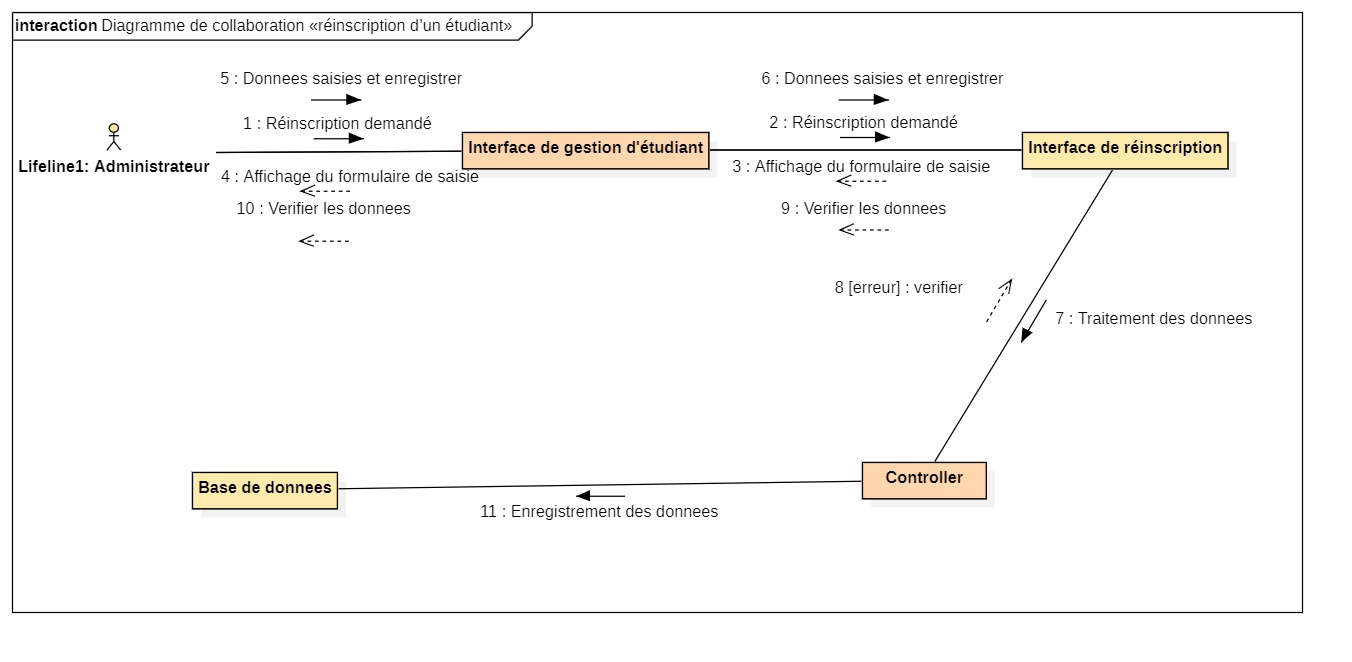
\includegraphics[width=13cm,height=10cm]{Diagrammecollaborationréinscriptiondunétudiant.jpg}
	\caption{Diagramme de collaboration «réinscription d' un étudiant» .}
	\label{fig:Diagramme de collaboration réinscription d' un étudiant  }
\end{figure}
\FloatBarrier
{\Large \color{cyan} Description des entités : Diagramme de collaboration «réinscription d' un étudiant»}

Un diagramme de collaboration est un diagramme d'interactions, représentation simplifiée d'un diagramme de séquence se concentrant sur les échanges de messages entre les objets, et où la chronologie n'intervient que de façon annexe.\\
Cela consiste en un graphe dont les nœuds sont des objets et les arcs (numérotés selon la chronologie) et les échanges entre ces objets.


\clearpage

\subsubsection{ Interface : Authentification  }
l'interface d'identification à spécialement les mails de l'administrateur pour que si l'utilisateur est un enseignant  et il veut impliqué dans l'interface de Ulearn comme un enseignant il faut envoyer un email pour vérifier ses capasite .

\begin{figure}[ht]
	\centering
	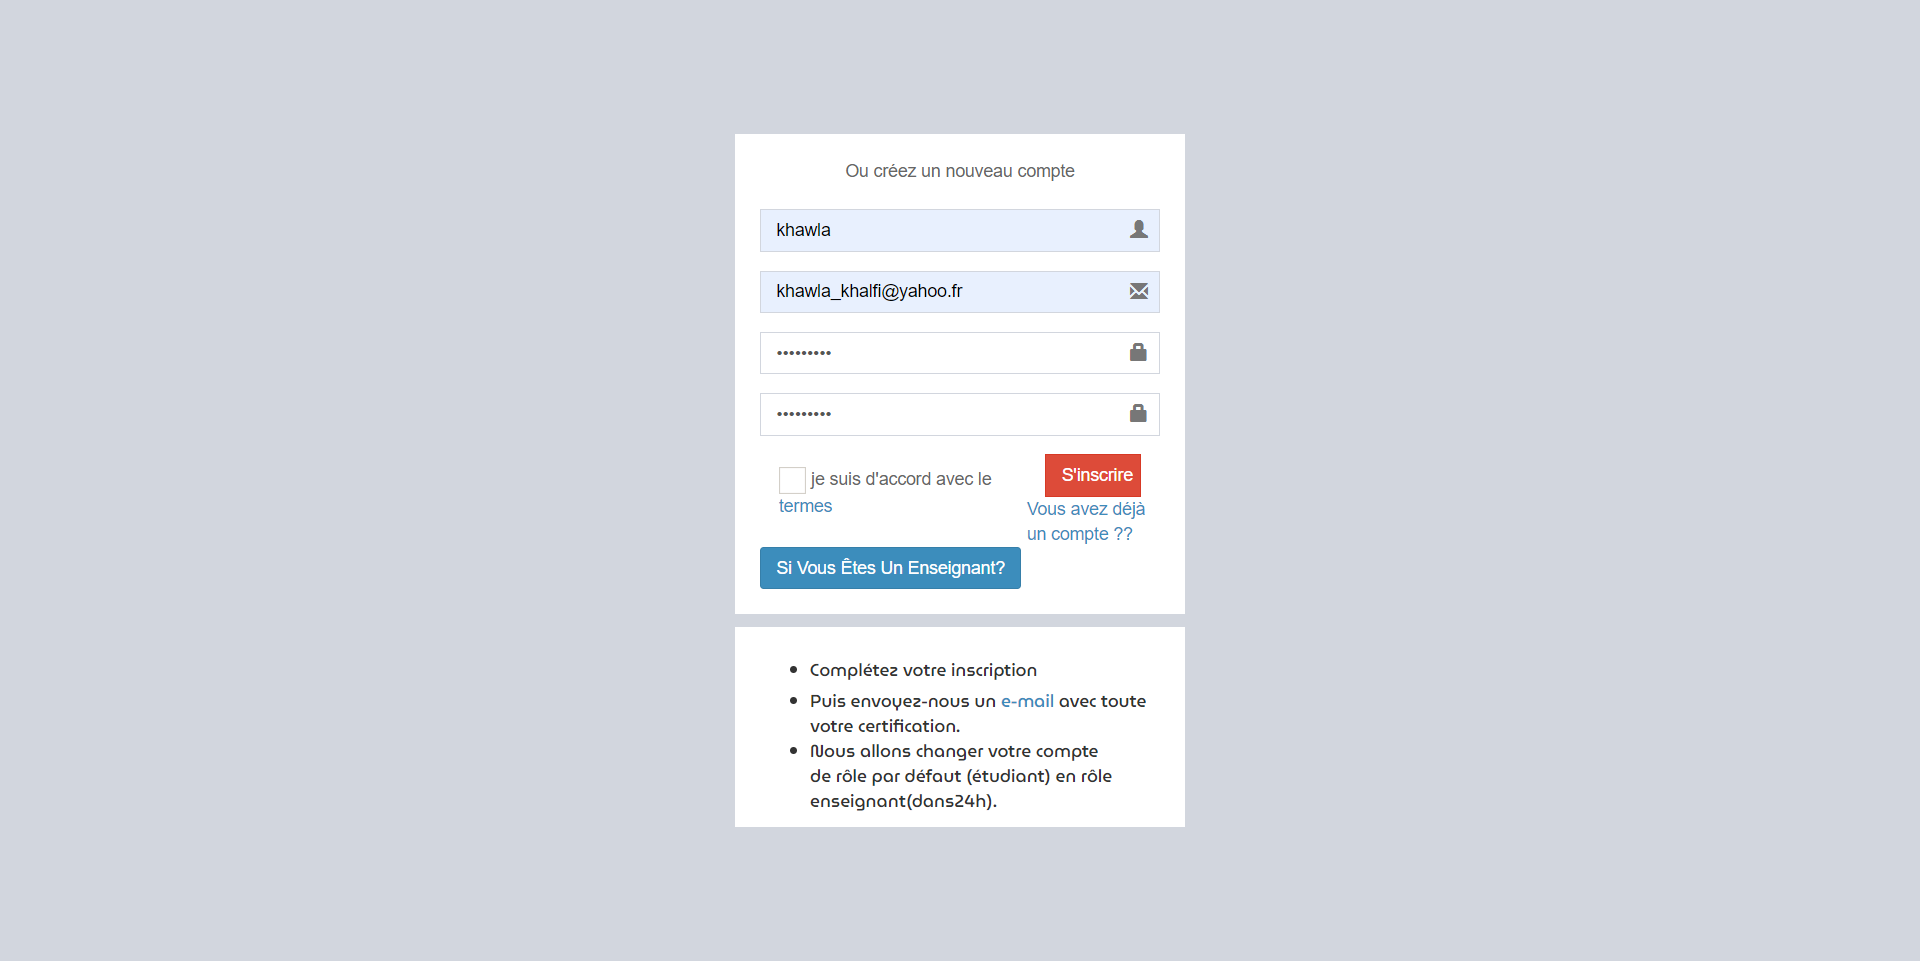
\includegraphics[width=18cm,height=8cm]{inscription.png}
	\caption{l'interface d'inscription avec les mails de vérification.}
	\label{fig:l'interface d'inscription avec les mails de vérification }
\end{figure}


\begin{figure}[ht]
	\centering
	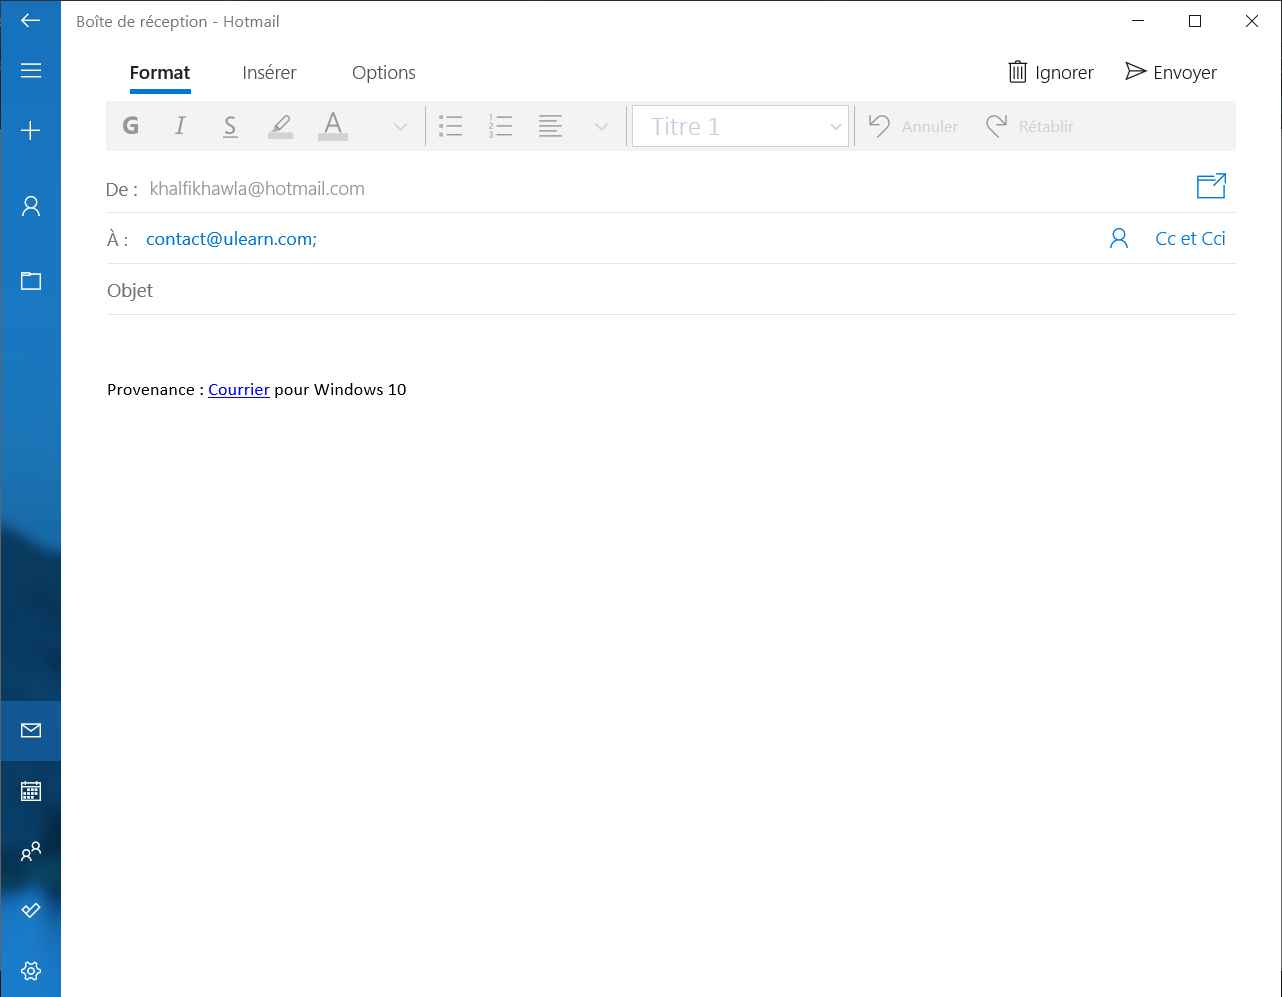
\includegraphics[width=10cm,height=6.2cm]{sbahcbLIFEQ.png}
	\caption{le message envoyé.}
	\label{fig:le message envoyé }
\end{figure}
\clearpage
\subsection{item 3 : Gestion des rôles utilisateurs}
\subsubsection{Diagrammes de séquence système }

La figure ci-dessous, décrit les opérations relatives à la gestion des rôles utilisateurs.
\begin{figure}[ht]
	\centering
	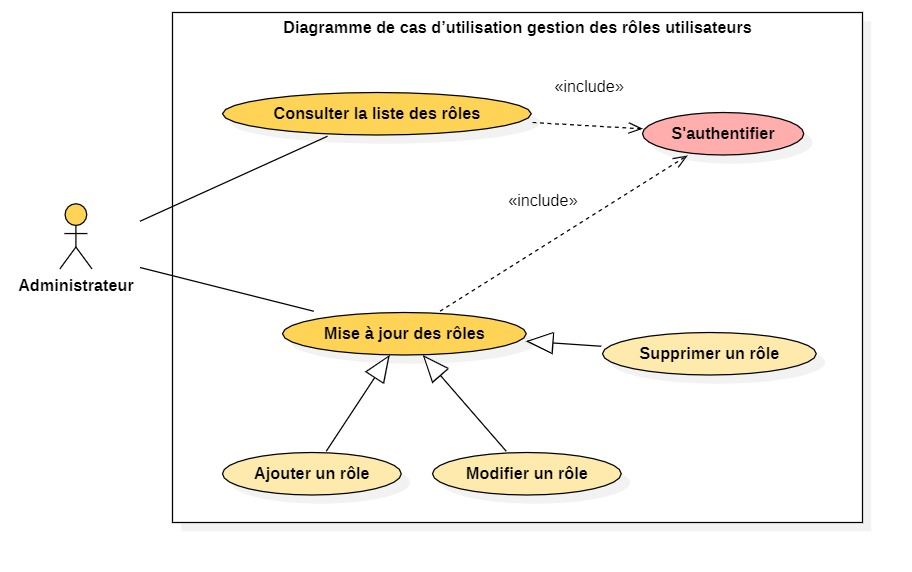
\includegraphics[width=13cm,height=12cm]{UseCaseDiagram1qw.jpg}
	\caption{Diagramme de cas d' utilisation gestion des rôles utilisateurs .}
	\label{fig:Diagramme de cas d utilisation gestion des rôles utilisateurs }
\end{figure}
\FloatBarrier
Ce diagramme de cas d’utilisation illustre les différentes opérations que l’administration peut effectuer pour gérer les rôles utilisateurs. L’administrateur doit s’authentifier
pour accéder à son espace. Il peut consulter la liste des rôles utilisateurs. Il peut aussi
ajouter, modifier ou supprimer un rôle. Toute opération effectuée, est enregistrée dans le
journal des opérations.
\clearpage
\subsubsection{Diagrammes de séquence système }


\begin{figure}[ht]
	\centering
	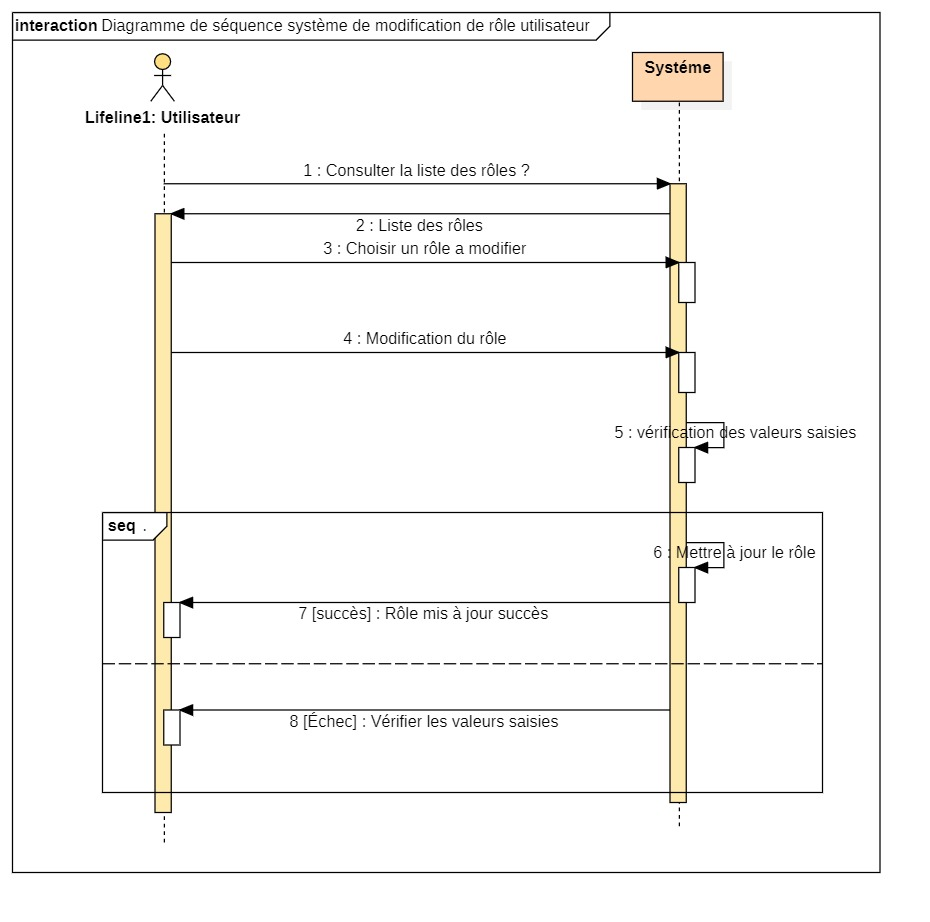
\includegraphics[width=13cm,height=15cm]{Diagséquencesystèmedemodificationderôleutilisateur.jpg}
	\caption{Diagramme de séquence système de modification de rôle utilisateur .}
	\label{fig:Diagramme de séquence système de modification de rôle utilisateur }
\end{figure}
\FloatBarrier

Pour modifier un rôle, l’administrateur consulte, tout d’abord, la liste des rôles qui
existent. Puis il peut choisir un rôle parmi la liste et met à jour les différents champs. Si
les valeurs des champs sont valides alors le rôle est mis à jour. Sinon si les valeurs ne sont
pas valides alors un message d’erreur apparaîtra à l’administrateur pour l’avertir.
\clearpage
\subsubsection{ Interface : Modification de rôle  }
les figures ci-dessous les représentent interfaces  de gérer les rôles des utilisateur à partir d'un administrateur .
\begin{figure}[ht]
	\centering
	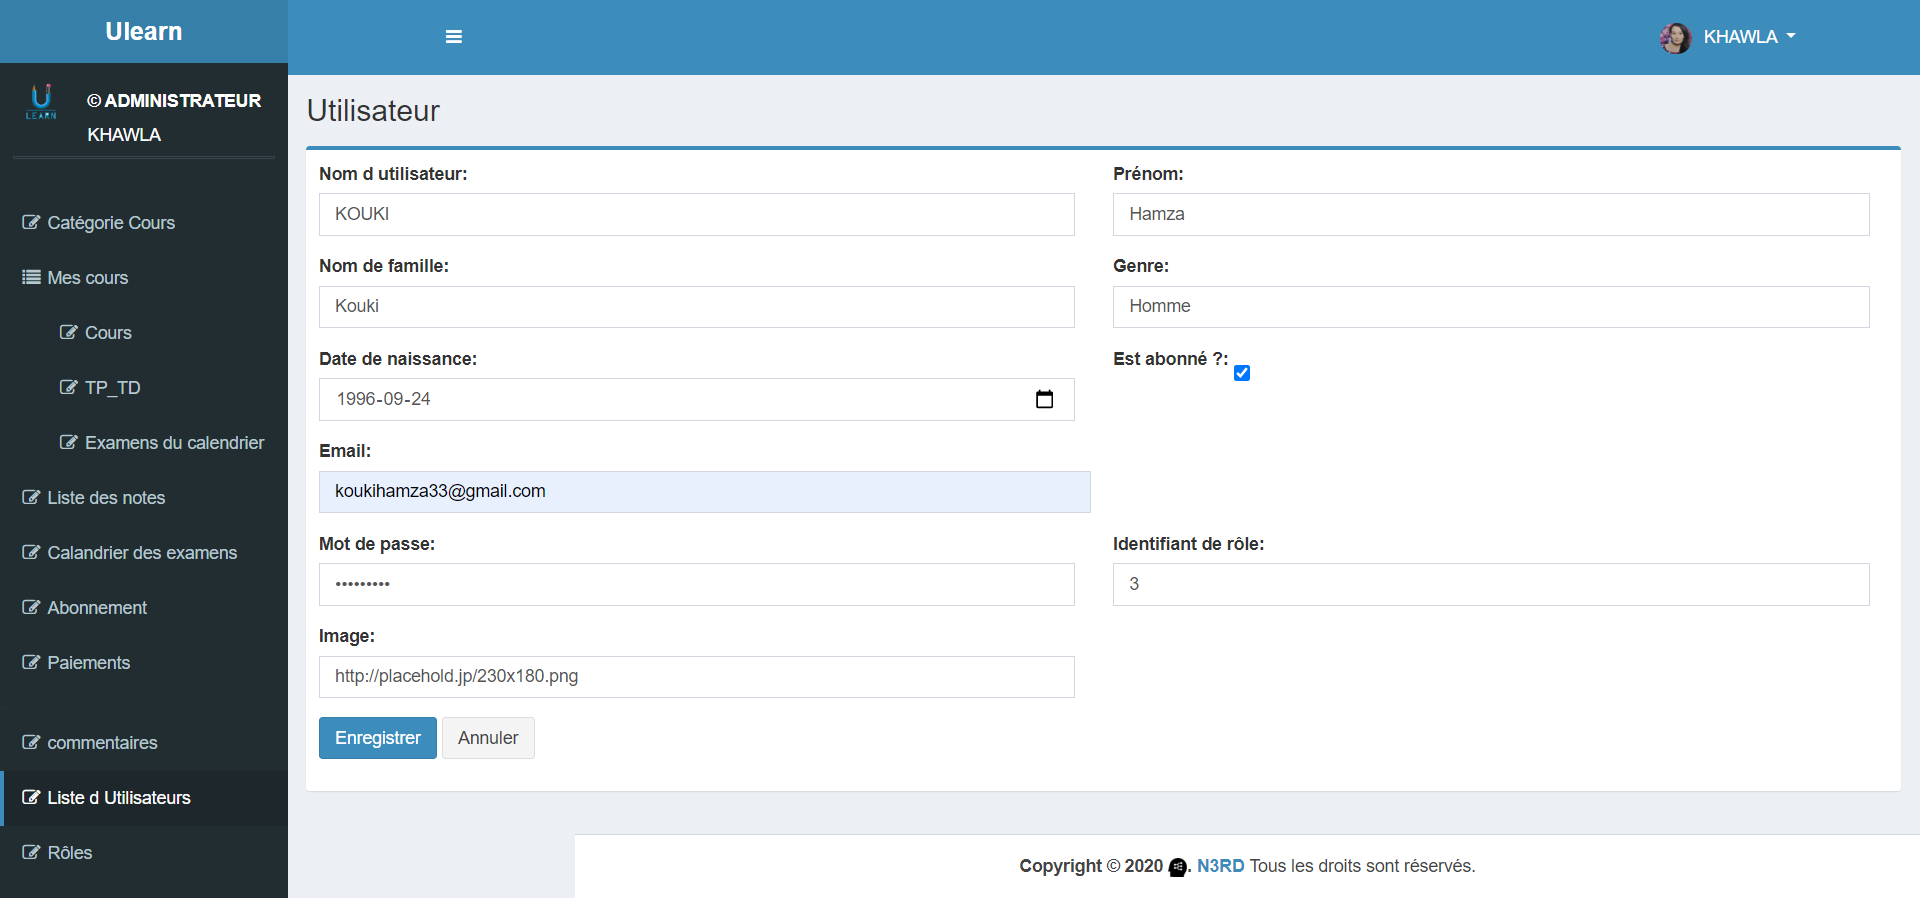
\includegraphics[width=13cm,height=10cm]{FGHt.png}
	\caption{Interface : Modification un rôle d'un utilisateur.}
	\label{fig:Modification de rôle1}
\end{figure}
\FloatBarrier
\begin{figure}[ht]
	\centering
	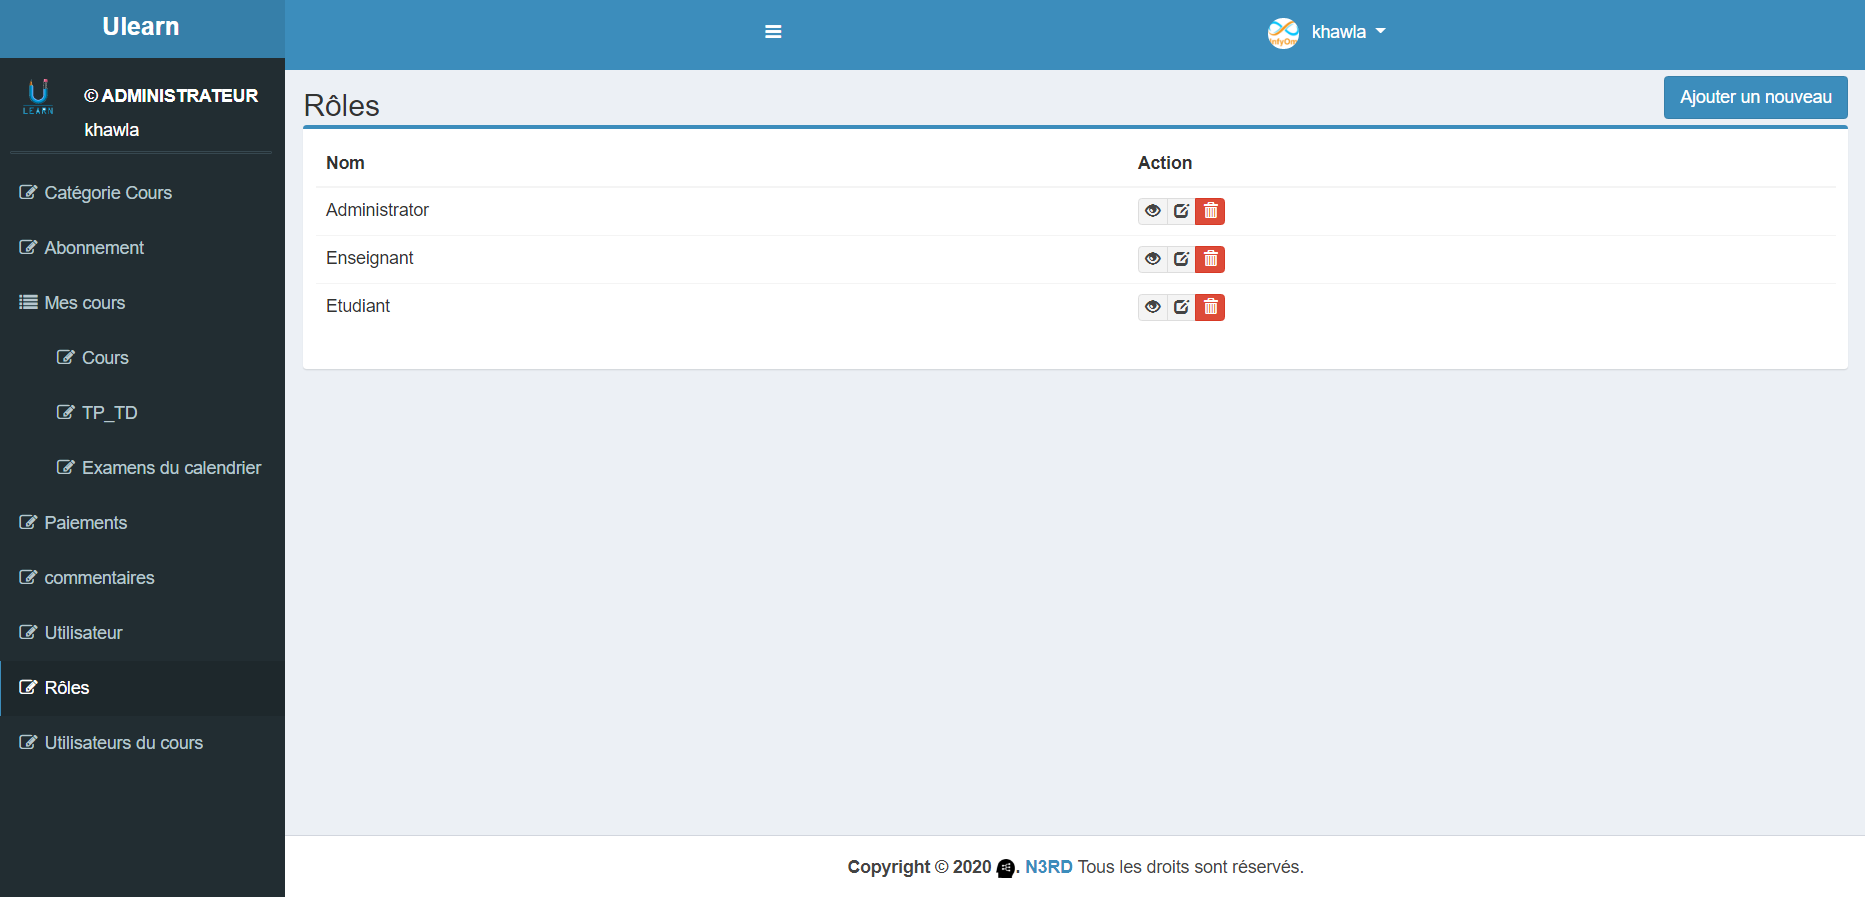
\includegraphics[width=13cm,height=4cm]{QVI.png}
	\caption{Interface : Modification, Ajouter un rôle .}
	\label{fig:2 }
\end{figure}
\FloatBarrier


\clearpage
%{+++++++++++++++++un autre section+++++++++++++++++++ }
%{+++++++++++++++++un autre section+++++++++++++++++++ }
%{+++++++++++++++++un autre section+++++++++++++++++++ }
%{+++++++++++++++++un autre section+++++++++++++++++++ }
\section{Sprint 3 : Enseignants }
\label{sec:conception}

\begin{fquote}
	Ce premier sprint s’étale sur 18 jours et se décompose en 3 items
\end{fquote}
\smallskip
\begin{itemize}[label=$\diamond$]
	\item Gérer les catégories / les cours 
	
	\item  gère les Tp/Td
	\item  Gérer l'évaluation
	
\end{itemize}
\medskip
\medskip
\medskip
\medskip
\medskip
\medskip
\medskip
\medskip
\medskip
\medskip
\medskip
\begin{figure}[ht]
	\centering
	\includegraphics[width=13cm,height=10cm]{Décompositionsprint3enItems.png}
	\caption{Décomposition sprint 3 en Items.}
	\label{fig:Décomposition srint 3 en Items}
\end{figure}
\FloatBarrier
\clearpage


%{+++++++++++++++++un autre section+++++++++++++++++++ }
%{+++++++++++++++++	\item  gère les Tp/Tds +++++++++++++++++++ }
%{+++++++++++++++++un autre section+++++++++++++++++++ }
%{+++++++++++++++++un autre section+++++++++++++++++++ }






\begin{table}[]
	{\Large\color{cyan} Le backlog du sprint 3 est le suivant :}\\
	
	\begin{tabular}{|l|l|l|l|}
		\hline 
		\rowcolor{-blue!20!red}{Item}                         & \textbf{User Story}                                                   & \textbf{Description}                                                                                              & \textbf{Priorité} \\ \hline
		\begin{tabular}[c]{@{}l@{}}\textbf{Gérer  }\\ \textbf{l'évaluation  } \end{tabular}                & \begin{tabular}[c]{@{}l@{}}Gérer\\ l'évaluationl  \end{tabular}                                                         & \begin{tabular}[c]{@{}l@{}}En tant que je suis un enseignant \\je peux accéder à l'espace d'évaluation\\ et je peux modifier , créer\\ ou bien supprimer un évaluation\\ d'un étudiant .\\cette évaluation contient le résultat \\d'un étudiant , une remarque ,le type de\\ catégorie  et le nom de l'étudiant .\end{tabular} & 2                 \\ \hline
		\multirow{4}{*}{\begin{tabular}[c]{@{}l@{}}\textbf{Gérer  }\\ \textbf{les ressources  }\\ \textbf{ et les liens d'}\\ \textbf{apprentissage } \end{tabular}}
		
		
		
	
		
		
		
		 & \begin{tabular}[c]{@{}l@{}}Gérer les\\ catégoriesl \\ \end{tabular}       & \begin{tabular}[c]{@{}l@{}}En tant que je suis à l'enseignant\\ je peux gérer les catégories :\\ ajouter modifier et supprimer\end{tabular}                    & 4                 \\ \cline{2-4} 
		& \begin{tabular}[c]{@{}l@{}}Gérer les\\  cours \\   \end{tabular}                                                       & \begin{tabular}[c]{@{}l@{}}En tant que je suis à l'enseignant\\ je peux gérer les cours :\\ ajouter modifier et supprimer\end{tabular}                     &     2              
	                       \\ \hline
		
		\begin{tabular}[c]{@{}l@{}}\textbf{gère les  }\\ \textbf{Tp/Td } \end{tabular}                   & \begin{tabular}[c]{@{}l@{}}gère les  \\ Tp/Td  \end{tabular}                                                           & \begin{tabular}[c]{@{}l@{}}	En tant qu'utilisateur, je peux ajouter \\Tp/Td  .\end{tabular}                                    & 3    \\ \hline
	\end{tabular}

	
	\caption{Tables Backlog du sprint 3}
	\label{Tables Backlog du sprint 3}
\end{table}


\begin{table}[h]
	{\Large\color{cyan} les user stories de sprint 3:}\\
	
	\begin{center}
		\begin{tabular}{>{\begin{bf} } c <{\end{bf}}ccc}
			
			\rowcolor{-blue!20!red}ID U.S & \begin{bf}User Story \end{bf}  & \\
			
			1 &en tant que je suis un enseignant je peux remplir   \\
		& le formulaire  de création d'un catégorie
		\\
			& \\	2 &en tant que je suis un enseignant je peux remplir   \\
			& le formulaire  de création d'un cours
			\\
			3 & en tant que je suis un enseignant je peux \\
			& je peux ajouter Tp/Td 
			\\
				4 & en tant que je suis un enseignant je peux \\
			&  remplir le formulaire d'évaluation d'un étudiant dans mon cours
			\\
			
			
			
		\end{tabular}
	\end{center}
	\caption{Tables  "les user stories de sprint 3"}
	\label{les user stories de sprint 3}
\end{table}


\clearpage

\clearpage
%{+++++++++++++++++un autre section+++++++++++++++++++ }
%{+++++++++++++++++un autre section+++++++++++++++++++ }
%{+++++++++++++++++un autre section+++++++++++++++++++ }
%{+++++++++++++++++un autre section+++++++++++++++++++ }
\subsection{item 1 : Gérer les catégories / les cours}

\subsubsection{Diagramme de cas d’utilisation  détaillé «le rôle d'un enseignant dans le plate-forme» }

\begin{figure}[ht]
	\centering
	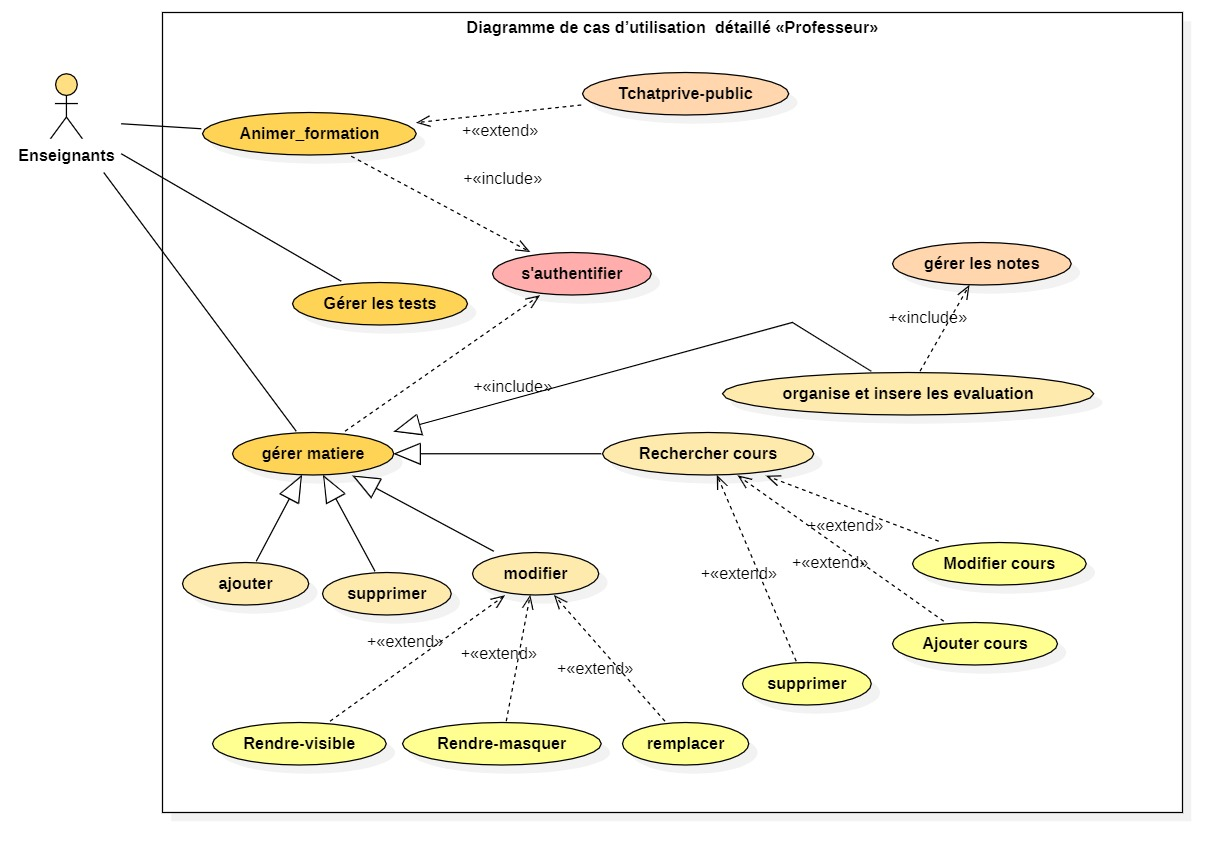
\includegraphics[width=18cm,height=8cm]{DiagrammedecasutilisationdétailléProfesseur.jpg}
	\caption{Diagramme de cas d' utilisation  détaillé «Professeur» .}
	\label{fig:Diagramme de cas d' utilisation  détaillé Professeur  }
\end{figure}

%{+++++++++++++++++un autre section+++++++++++++++++++ }
%{+++++++++++++++++un autre section+++++++++++++++++++ }
%{+++++++++++++++++un autre section+++++++++++++++++++ }
%{+++++++++++++++++un autre section+++++++++++++++++++ }
%{+++++++++++++++++un autre section+++++++++++++++++++ }
%{+++++++++++++++++un autre section+++++++++++++++++++ }
%{+++++++++++++++++un autre section+++++++++++++++++++ }
%{+++++++++++++++++un autre section+++++++++++++++++++ }
%{+++++++++++++++++un autre section+++++++++++++++++++ }
%{+++++++++++++++++un autre section+++++++++++++++++++ }
%{+++++++++++++++++un autre section+++++++++++++++++++ }
%{+++++++++++++++++un autre section+++++++++++++++++++ }
%{+++++++++++++++++un autre section+++++++++++++++++++ }
%{+++++++++++++++++un autre section+++++++++++++++++++ }
%{+++++++++++++++++un autre section+++++++++++++++++++ }
%{+++++++++++++++++un autre section+++++++++++++++++++ }

\subsubsection{Diagramme des cas d' utilisation  Gérer les cours }
\begin{figure}[ht]
	\centering
	\includegraphics[width=17cm,height=6cm]{CasutilisationGérerlescours.jpg}
	\caption{Diagramme des cas d' utilisation « Gérer les cours » .}
	\label{fig:Diagramme des cas d' utilisation  Gérer les cours  }
\end{figure}
\FloatBarrier

\clearpage

%{+++++++++++++++++un autre section+++++++++++++++++++ }
%{+++++++++++++++++un autre section+++++++++++++++++++ }
%{+++++++++++++++++un autre section+++++++++++++++++++ }
%{+++++++++++++++++un autre section+++++++++++++++++++ }

\subsubsection{diagramme de séquences }
\begin{figure}[ht]
	\centering
	\includegraphics[width=13cm,height=11cm]{DiagrammedeséquenceGererlescours.jpg}
	\caption{Diagramme de séquence "Gerer les cours" .}
	\label{fig:Diagramme de séquence "Gerer les cours"  }
\end{figure}
\FloatBarrier
Aprés introduire le login et mot de passe l’enseignant peut gérer le cours (Modifier, Ajouter,
Supprimer) Cours, sinon il affiche un message "cours est in trouvée"

{\Large \color{cyan} Description détaillée: "Ajouter un cour"}
\begin{itemize}
	\item[$\bullet$] \textbf{Cas d’utilisation "Ajouter un cour" :} 
	\medskip
	\begin{itemize}
		\item \textit{\textbf{Objectif :}} Ajouter un cour	
		\item \textit{\textbf{Acteur :}}  l'enseignant
		\item \textit{\textbf{Pré-condition  :}} \\
		Le responsable s’identifie.\\
		Le responsable peut accéder à l’application.\\
		Module affichée.
		\item \textit{\textbf{Post-conditions   :}}ajouter les données de la cours à l'interface spécifiée .
		\item \textit{\textbf{Scénario nominal :}}
		\begin{enumerate}
			\item le responsable choisir la gestion de cours.
			\item le système afficher la liste des cours .
			\item le responsable clique sur le bouton ajouter nouveau .
			
			\item le système afficher un formulaire à remplir. 
			\item  Le responsable sélectionne une remplir ces
			informations, en validant l’opération d’ajout. 
			\item L’ajout de la cours est confirmé par le système :Message de confirmation de l'Ajouter  

		\end{enumerate}
		\item \textit{\textbf{Scénario alternative :}}
		\begin{enumerate}
			\item Tentative soldée par échec (informations existe et
			déjà enregistrés)
		\end{enumerate}
	\end{itemize}
\end{itemize}	
\bigskip


{\Large \color{cyan} Description détaillée: "Modifier un cour"}
\begin{itemize}
	\item[$\bullet$] \textbf{Cas d’utilisation "Modifier un cour" :} 
	\medskip
	\begin{itemize}
		\item \textit{\textbf{Objectif :}} Modifier un cour	
		\item \textit{\textbf{Acteur :}}  l'enseignant
		\item \textit{\textbf{Pré-condition  :}} \\
		Le responsable s’identifie.\\
		Le responsable peut accéder à l’application.\\
		Module affichée.
		\item \textit{\textbf{Post-conditions   :}}Le cours est déjà modifiée et enregistrée dans
		la base. 
		\item \textit{\textbf{Scénario nominal :}}
		\begin{enumerate}
			\item le responsable choisir la gestion de cours.
			\item le système afficher la liste des cours .
			\item le responsable clique sur le bouton Modifier .
			
			\item le système afficher le formulaire du cours. 
			\item  Le responsable sélectionne une modification. 
			\item La modificationde la cours est confirmé par le système. 
			\item Message de confirmation de La modificationde .
			
		\end{enumerate}
		\item \textit{\textbf{Scénario alternative :}}
		\begin{enumerate}
			\item Tentative soldée par échec (informations existe et
			déjà enregistrés)
		\end{enumerate}
	\end{itemize}
\end{itemize}	
\bigskip



%{+++++++++++++++++un autre section+++++++++++++++++++ }
%{+++++++++++++++++un autre section+++++++++++++++++++ }
%{+++++++++++++++++un autre section+++++++++++++++++++ }
%{+++++++++++++++++un autre section+++++++++++++++++++ }

\clearpage
\subsubsection{diagramme de séquences }
\begin{figure}[ht]
	\centering
	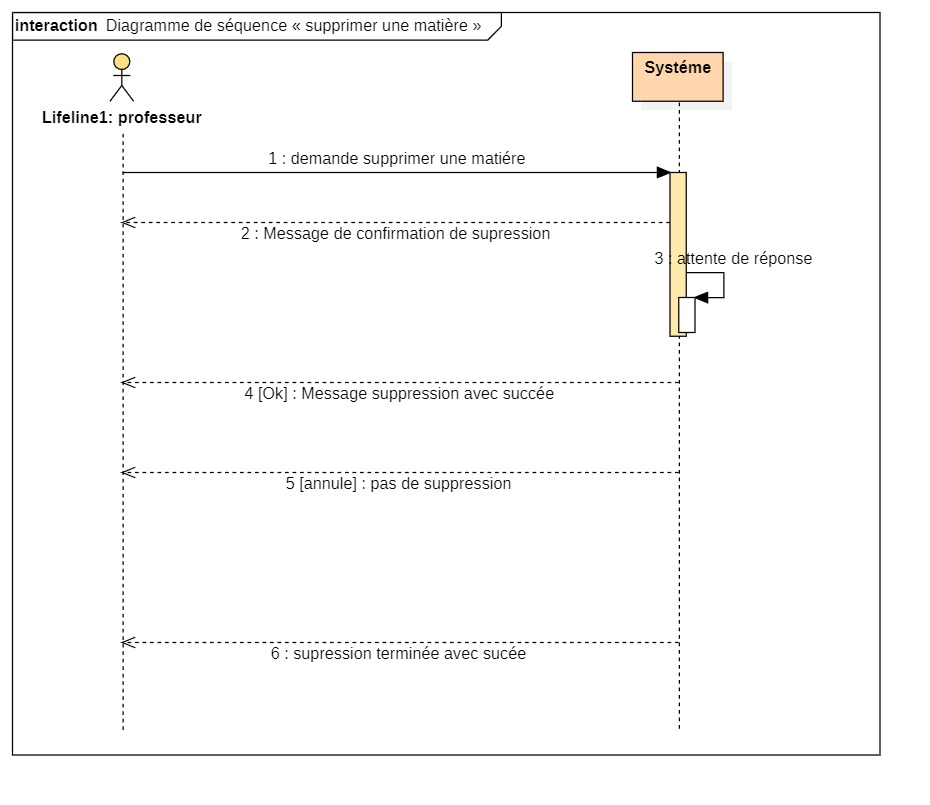
\includegraphics[width=13cm,height=7cm]{Diagrammedeséquencesupprimerunematière.jpg}
	\caption{ Diagramme de séquence « supprimer cours » .}
	\label{fig: Diagramme de séquence  supprimer cours   }
\end{figure}
\FloatBarrier



{\Large \color{cyan} Description détaillée: "supprimer cours"}
\begin{itemize}
	\item[$\bullet$] \textbf{Cas d’utilisation "supprimer cours" :} 
	\medskip
	\begin{itemize}
		\item \textit{\textbf{Objectif :}}supprimer cours	
		\item \textit{\textbf{Acteur :}}  l'enseignant
		\item \textit{\textbf{Pré-condition  :}} \\
		Le responsable s’identifie.\\
		Le responsable peut accéder à l’application.\\
		Module affichée.
		\item \textit{\textbf{Post-conditions   :}}Le module est déjà supprimé et enregistré dans la
		base.
		\item \textit{\textbf{Scénario nominal :}}
		\begin{enumerate}
			\item le responsable choisir la gestion de cours.
			\item le système afficher la liste des cours .
			\item le responsable choisir cours et cliquez sur le bouton Supprimer .
			
			\item le systèmea afficher un message pour le confirmation. 
			\item  Le responsable confirmé
			\item le systèmea afficher un message de le confirmation.
		\end{enumerate}
		\item \textit{\textbf{Scénario alternative :}}
		\begin{enumerate}
			\item Tentative soldée par échec (informations existe et
			déjà enregistrés)
		\end{enumerate}
	\end{itemize}
\end{itemize}	
\bigskip

\clearpage

%{+++++++++++++++++un autre section+++++++++++++++++++ }
%{+++++++++++++++++un autre section+++++++++++++++++++ }
%{+++++++++++++++++un autre section+++++++++++++++++++ }
%{+++++++++++++++++un autre section+++++++++++++++++++ }
\subsubsection{diagramme de séquences }
\begin{figure}[ht]
	\centering
	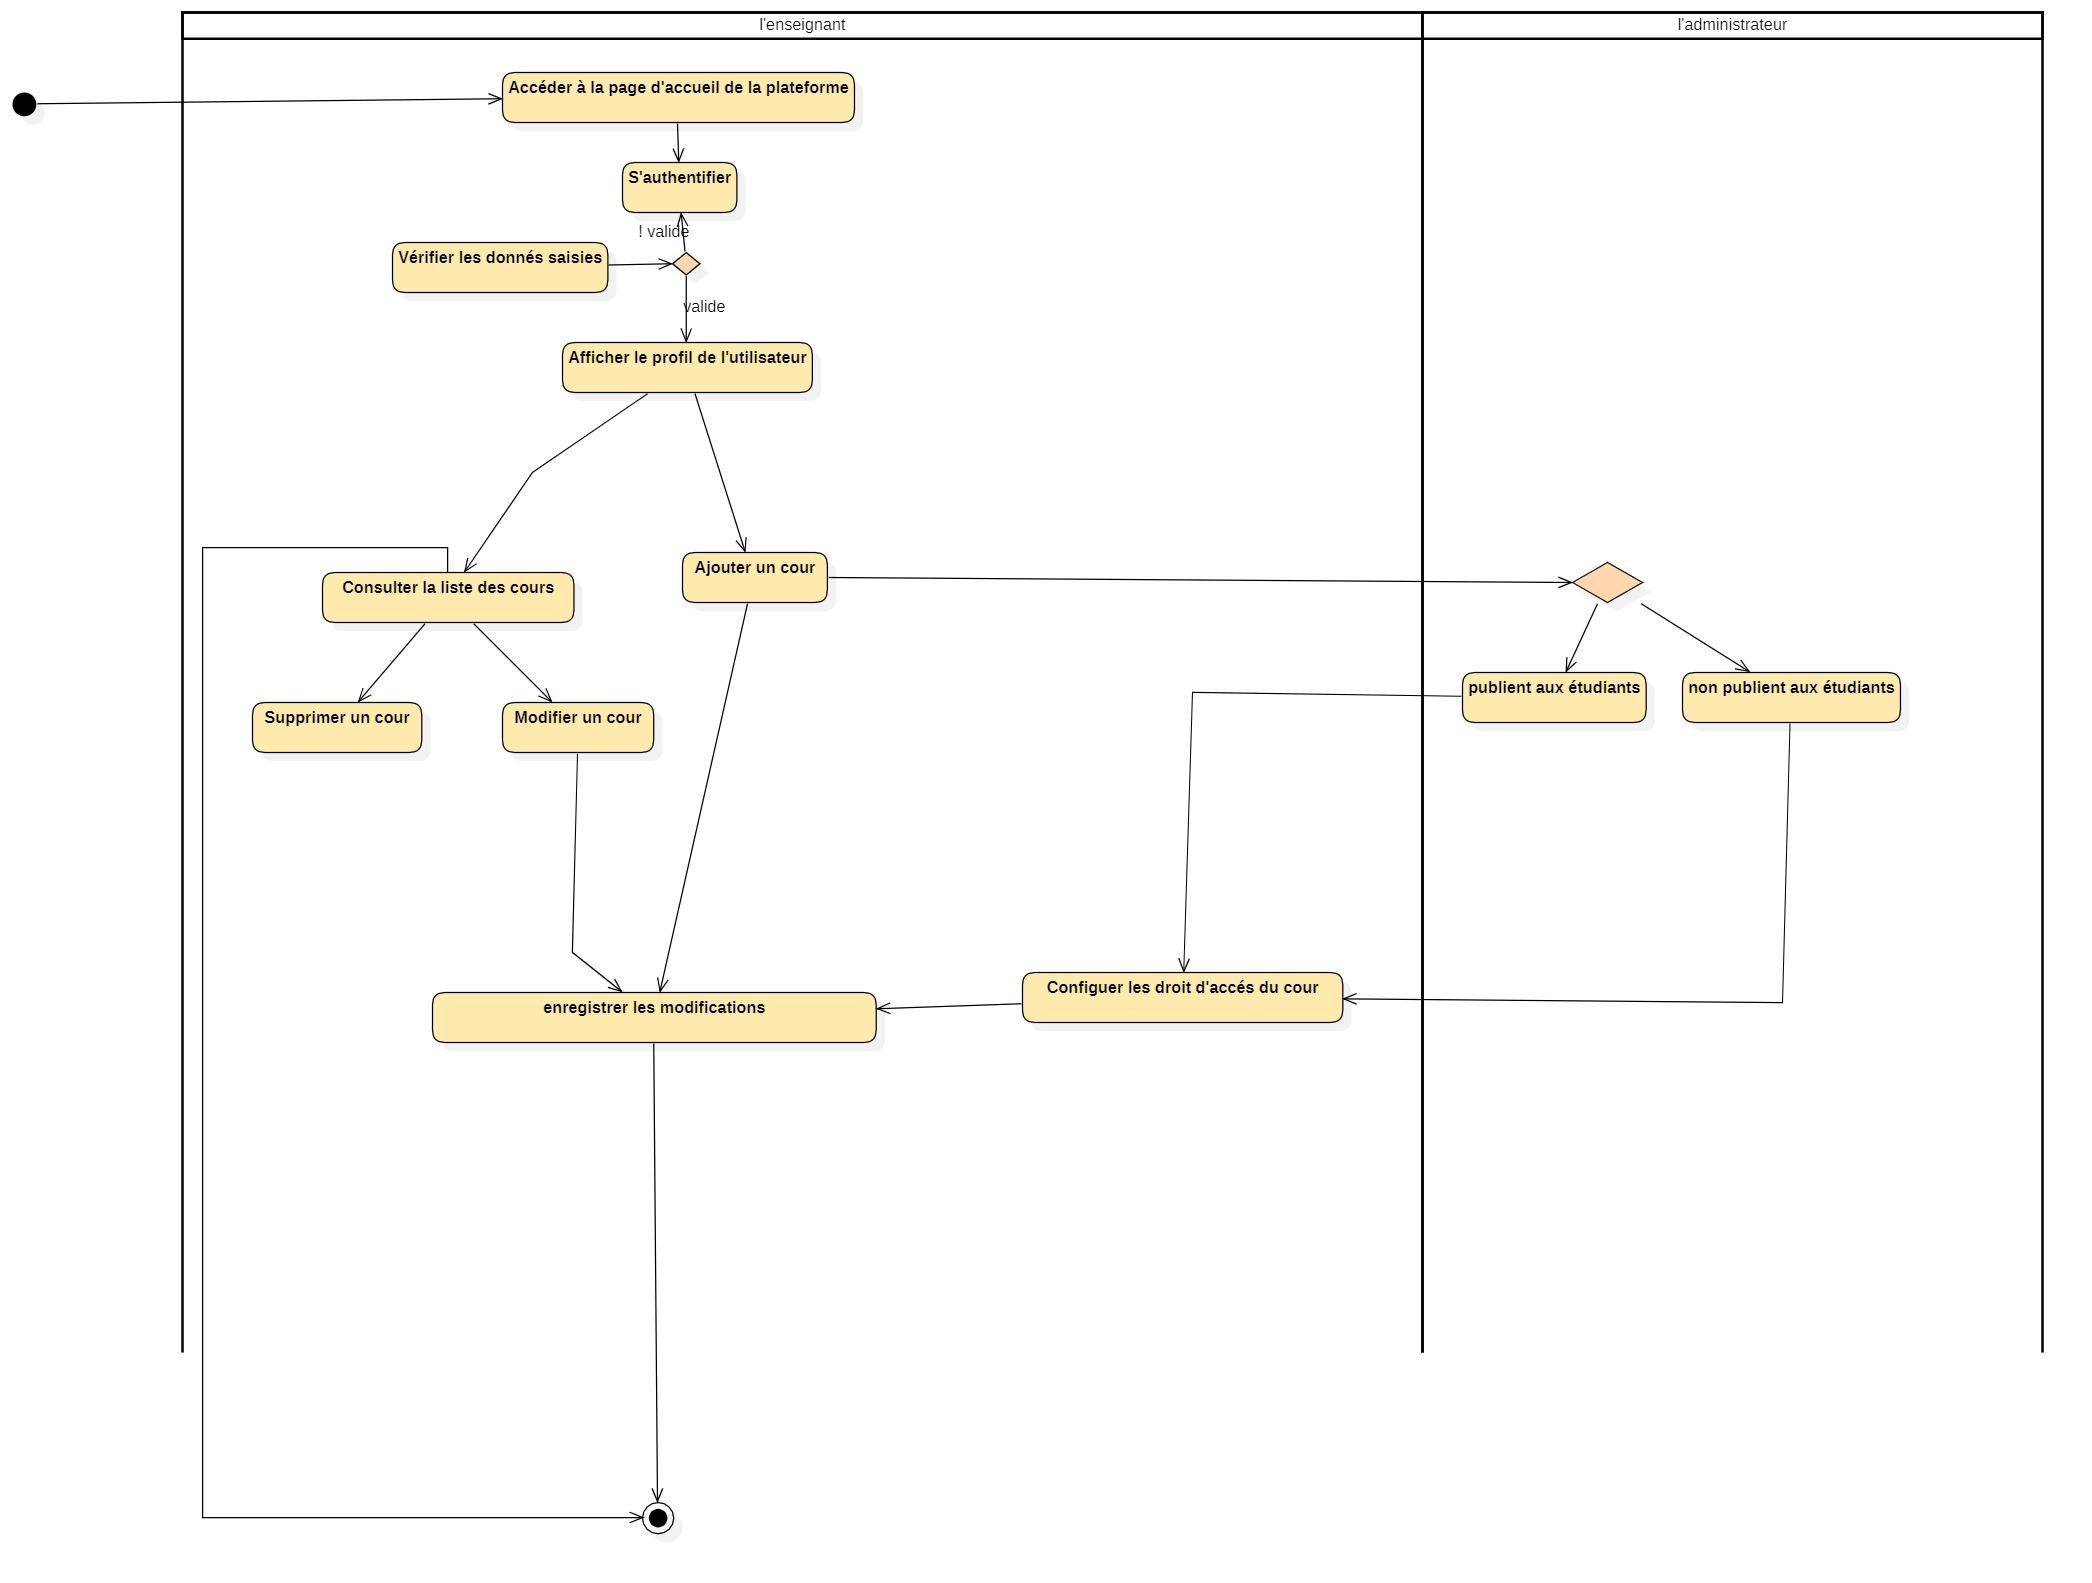
\includegraphics[width=16cm,height=14cm]{DiagrammeactivitésGérerlescou.jpg}
	\caption{Diagramme d' activités « Gérer les cours » .}
	\label{fig:Diagramme d' activités  Gérer les cours  }
\end{figure}
\FloatBarrier

{\Large \color{cyan} Description des entités:}\\
La figure ci-dessus illustre le déroulement séquentiel de la gestion des cours accomplis par un Enseignant.\\
Après avoir s’authentifié, un Enseignant peut ajouter, modifier ou supprimer un cours.\\
Au cas d’ajout ou de modification du cours, le tuteur doit ajouter cet évènement  partagé pour informer les apprenants du changement.
\clearpage

%{+++++++++++++++++un autre section+++++++++++++++++++ }
%{+++++++++++++++++un autre section+++++++++++++++++++ }
%{+++++++++++++++++un autre section+++++++++++++++++++ }
%{+++++++++++++++++un autre section+++++++++++++++++++ }
\subsubsection{Les Interfaces de : gérer les cours  }
Une fois authentifié,  l'enseignant peut accéder à son espace. \\
Il peut consulter la liste  des cours comme la figure suivante
, comme il peut soit voir les cours ou les modifier
via la liste affichée. \\
Il peut aussi aussi ajouter un nouveau cours à partir de  la clique sur le bouton «ajouter un nouveau». \\
à partir de cette clics la formulaire de la création d'un cours s'ouvre , il faut donc il faut que l'enseignant remplir le formulaire  pour créer un nouveau cours .\\
ci-dessous, illustrent ces opérations.
\medskip
\medskip
\medskip
\begin{figure}[ht]
	\centering
	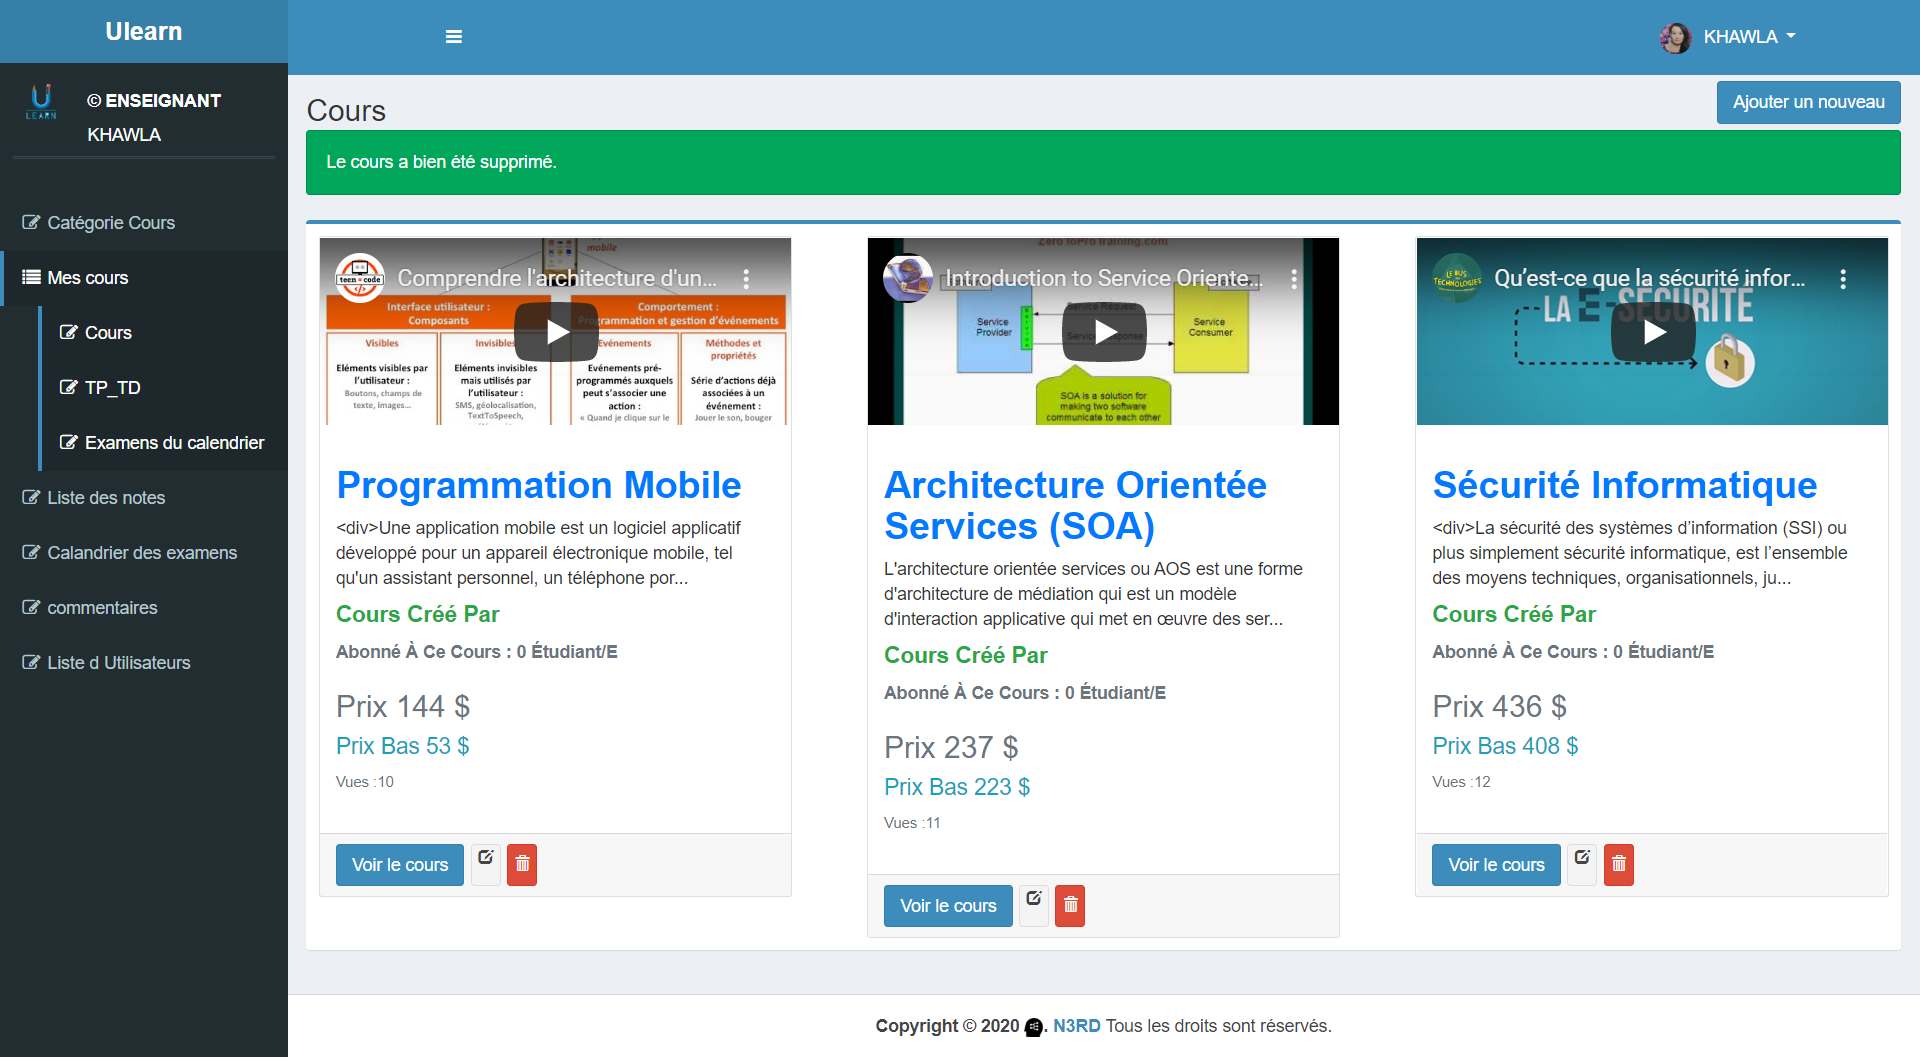
\includegraphics[width=15cm,height=13cm]{screencapture-localhost-8000-courses-2020-06-24-14_44_16.png}
	\caption{la liste des cours .}
	\label{fig:la liste des cours  }
\end{figure}
\FloatBarrier

%{+++++++++++++++++un autre section+++++++++++++++++++ }
%{+++++++++++++++++un autre section+++++++++++++++++++ }
%{+++++++++++++++++un autre section+++++++++++++++++++ }
%{+++++++++++++++++un autre section+++++++++++++++++++ }

\begin{figure}[ht]
	\centering
	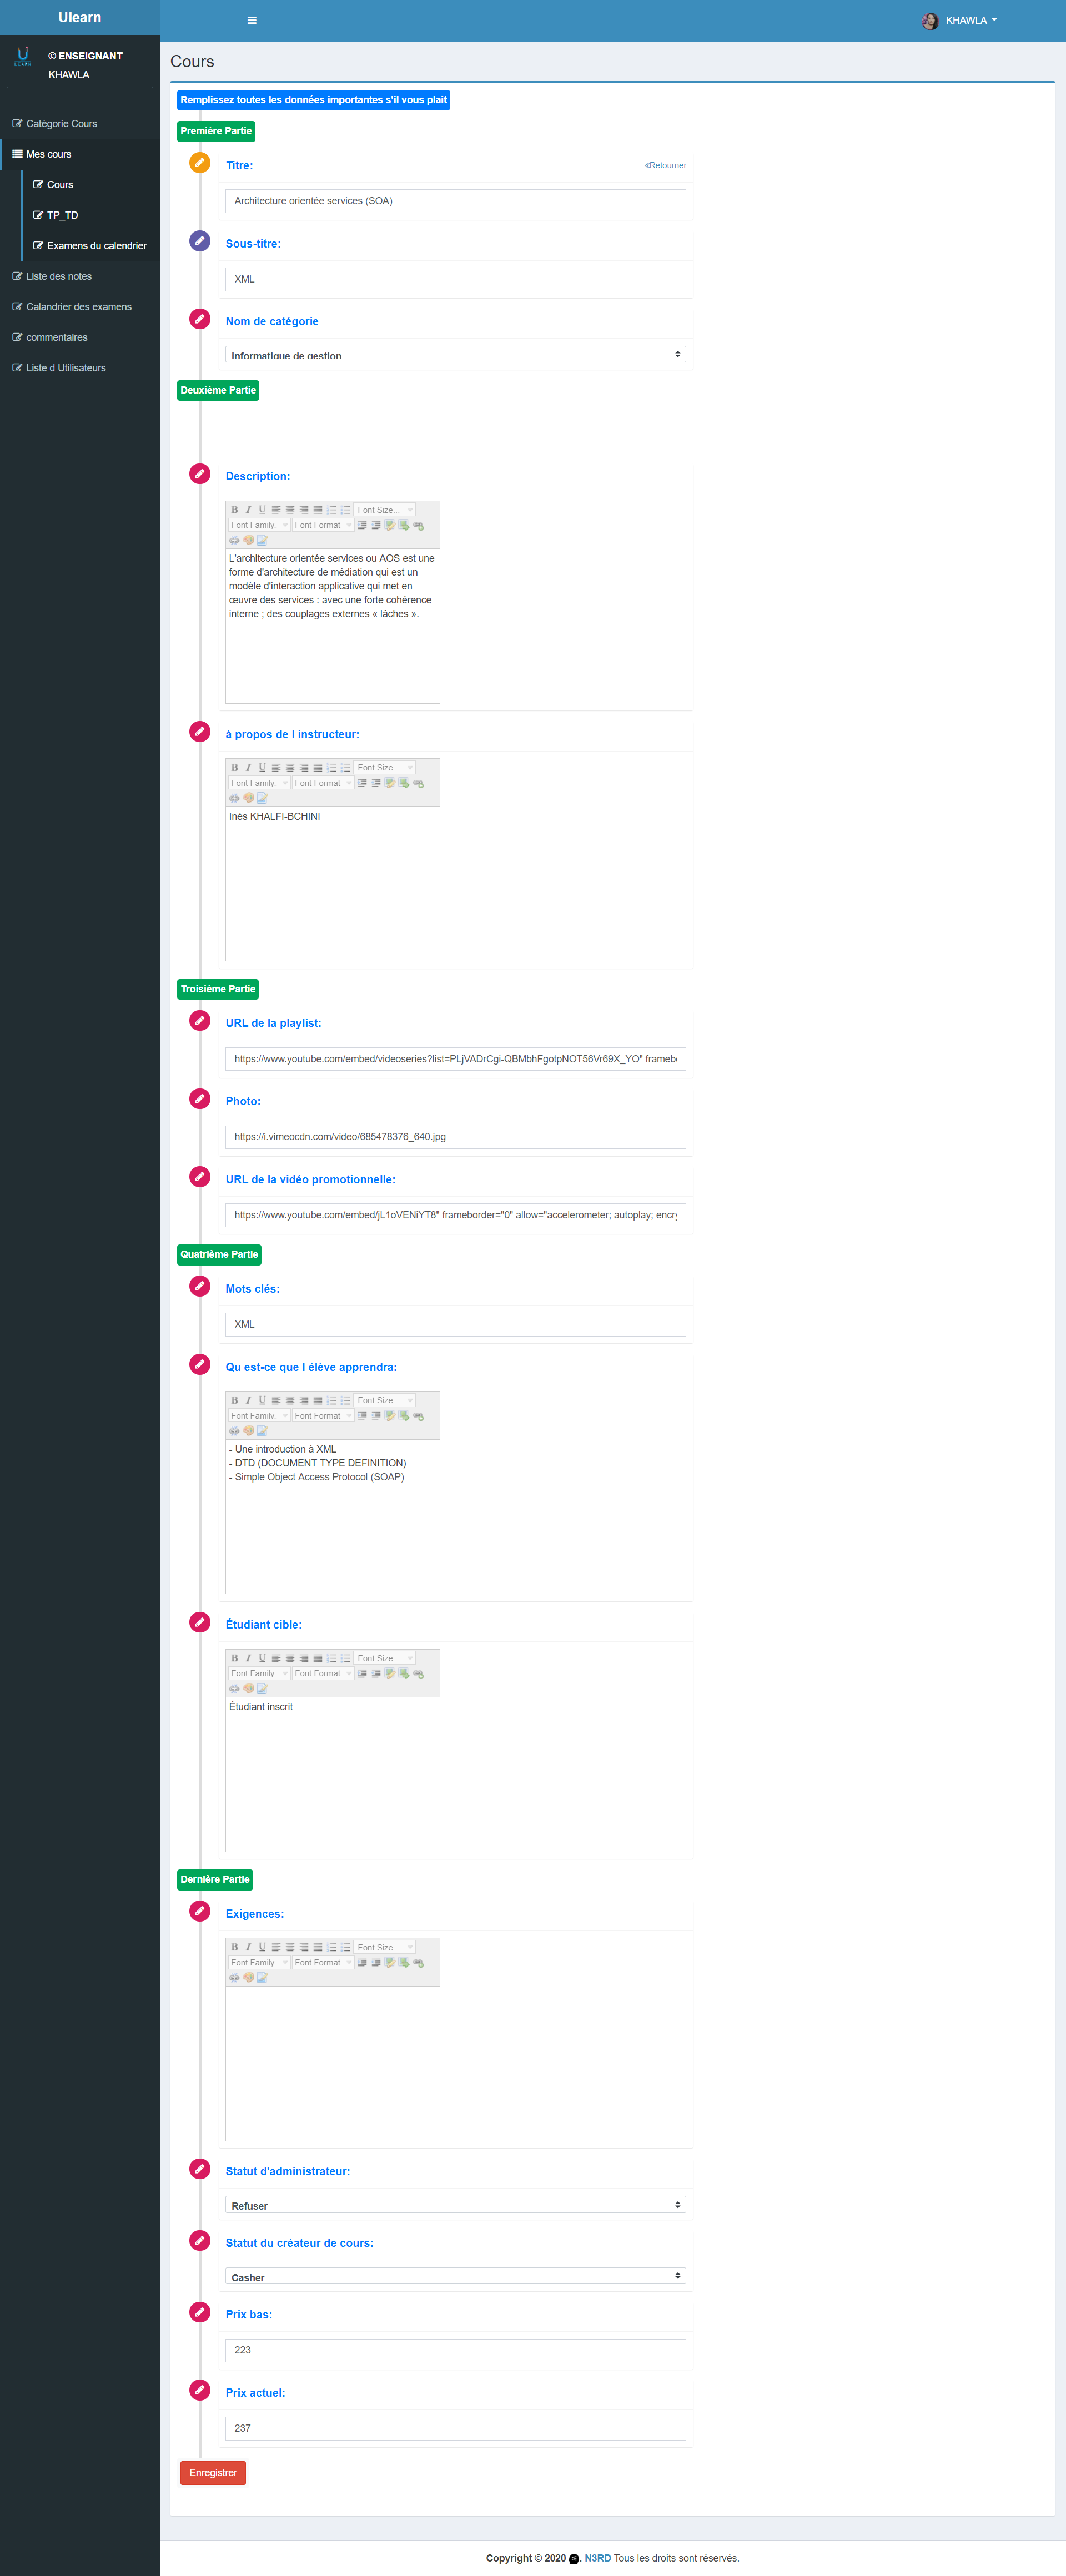
\includegraphics[width=15cm,height=20cm]{screencapture-localhost-8000-courses-11-edit-2020-06-24-14_43_47.png}
	\caption{la formulaire de création un cours .}
	\label{fig: la formulaire de création un cours  }
\end{figure}
\FloatBarrier
%{+++++++++++++++++un autre section+++++++++++++++++++ }
%{+++++++++++++++++un autre section+++++++++++++++++++ }
%{+++++++++++++++++un autre section+++++++++++++++++++ }
%{+++++++++++++++++un autre section+++++++++++++++++++ }
\clearpage

%{+++++++++++++++++un autre section+++++++++++++++++++ }
%{+++++++++++++++++un autre section+++++++++++++++++++ }
%{+++++++++++++++++un autre section+++++++++++++++++++ }
%{+++++++++++++++++un autre section+++++++++++++++++++ }
%{+++++++++++++++++un autre section+++++++++++++++++++ }
%{+++++++++++++++++un autre section+++++++++++++++++++ }
%{+++++++++++++++++un autre section+++++++++++++++++++ }
%{+++++++++++++++++un autre section+++++++++++++++++++ }
%{+++++++++++++++++un autre section+++++++++++++++++++ }
%{+++++++++++++++++un autre section+++++++++++++++++++ }
%{+++++++++++++++++un autre section+++++++++++++++++++ }
%{+++++++++++++++++un autre section+++++++++++++++++++ }
%{+++++++++++++++++un autre section+++++++++++++++++++ }
%{+++++++++++++++++un autre section+++++++++++++++++++ }
%{+++++++++++++++++un autre section+++++++++++++++++++ }
%{+++++++++++++++++un autre section+++++++++++++++++++ }

\subsubsection{Diagramme des cas d' utilisation  Gérer les catégories }
\begin{figure}[ht]
	\centering
	\includegraphics[width=17cm,height=6cm]{CasutilisationffGérerlescours.jpg}
	\caption{Diagramme des cas d' utilisation « Gérer les catégories » .}
	\label{fig:Diagramme des cas d' utilisation Gérer les catégories  }
\end{figure}
\FloatBarrier



%{+++++++++++++++++un autre section+++++++++++++++++++ }
%{+++++++++++++++++un autre section+++++++++++++++++++ }
%{+++++++++++++++++un autre section+++++++++++++++++++ }
%{+++++++++++++++++un autre section+++++++++++++++++++ }

\subsubsection{diagramme de séquences }
\begin{figure}[ht]
	\centering
	\includegraphics[width=13cm,height=8cm]{DiagrammedeséqsfuenceGererlescours.jpg}
	\caption{Diagramme de séquence "Gérer les catégories" .}
	\label{fig:Diagramme de séquence "Gérer les catégories"  }
\end{figure}
\FloatBarrier
\clearpage
Aprés introduire le login et mot de passe l’enseignant peut gérer les catégories (Modifier, Ajouter,
Supprimer) catégories , sinon il affiche un message "catégorie est in trouvée"

{\Large \color{cyan} Description détaillée: "Ajouter catégorie"}
\begin{itemize}
	\item[$\bullet$] \textbf{Cas d’utilisation "Ajouter catégorie" :} 
	\medskip
	\begin{itemize}
		\item \textit{\textbf{Objectif :}} Ajouter catégorie	
		\item \textit{\textbf{Acteur :}}  l'enseignant
		\item \textit{\textbf{Pré-condition  :}} \\
		Le responsable s’identifie.\\
		Le responsable peut accéder à l’application.\\
		Module affichée.
		\item \textit{\textbf{Post-conditions   :}}ajouter les données de la catégorie à l'interface spécifiée .
		\item \textit{\textbf{Scénario nominal :}}
		\begin{enumerate}
			\item le responsable choisir la gestion de catégories.
			\item le système afficher la liste des catégories .
			\item le responsable clique sur le bouton ajouter nouveau .
			
			\item le système afficher un formulaire à remplir. 
			\item  Le responsable sélectionne une remplir ces
			informations, en validant l’opération d’ajout. 
			\item L’ajout de la catégories est confirmé par le système :Message de confirmation de l'Ajouter  
			
		\end{enumerate}
		\item \textit{\textbf{Scénario alternative :}}
		\begin{enumerate}
			\item Tentative soldée par échec (informations existe et
			déjà enregistrés)
		\end{enumerate}
	\end{itemize}
\end{itemize}	
\bigskip


{\Large \color{cyan} Description détaillée: "Modifier catégorie"}
\begin{itemize}
	\item[$\bullet$] \textbf{Cas d’utilisation "Modifier catégorie" :} 
	\medskip
	\begin{itemize}
		\item \textit{\textbf{Objectif :}} Modifier catégorie	
		\item \textit{\textbf{Acteur :}}  l'enseignant
		\item \textit{\textbf{Pré-condition  :}} \\
		Le responsable s’identifie.\\
		Le responsable peut accéder à l’application.\\
		Module affichée.
		\item \textit{\textbf{Post-conditions   :}}La catégorie est déjà modifiée et enregistrée dans
		la base. 
		\item \textit{\textbf{Scénario nominal :}}
		\begin{enumerate}
			\item le responsable choisir la gestion de catégorie.
			\item le système afficher la liste des catégories .
			\item le responsable clique sur le bouton Modifier .
			
			\item le système afficher le formulaire du catégorie. 
			\item  Le responsable sélectionne une modification. 
			\item La modificationde la catégorie est confirmé par le système. 
			\item Message de confirmation de La modificationde .
			
		\end{enumerate}
		\item \textit{\textbf{Scénario alternative :}}
		\begin{enumerate}
			\item Tentative soldée par échec (informations existe et
			déjà enregistrés)
		\end{enumerate}
	\end{itemize}
\end{itemize}	
\bigskip

%{+++++++++++++++++un autre section+++++++++++++++++++ }
%{+++++++++++++++++un autre section+++++++++++++++++++ }
%{+++++++++++++++++un autre section+++++++++++++++++++ }
%{+++++++++++++++++un autre section+++++++++++++++++++ }
%{+++++++++++++++++un autre section+++++++++++++++++++ }
%{+++++++++++++++++un autre section+++++++++++++++++++ }
%{+++++++++++++++++un autre section+++++++++++++++++++ }
%{+++++++++++++++++un autre section+++++++++++++++++++ }
%{+++++++++++++++++un autre section+++++++++++++++++++ }
%{+++++++++++++++++un autre section+++++++++++++++++++ }
%{+++++++++++++++++un autre section+++++++++++++++++++ }
%{+++++++++++++++++un autre section+++++++++++++++++++ }


\subsubsection{diagramme de séquences }
\begin{figure}[ht]
	\centering
	\includegraphics[width=13cm,height=11cm]{Diesupprimerunematière.jpg}
	\caption{ Diagramme de séquence « supprimer catégorie » .}
	\label{fig: Diagramme de séquence  supprimer catégorie   }
\end{figure}
\FloatBarrier

\clearpage

{\Large \color{cyan} Description détaillée: "supprimer catégorie"}
\begin{itemize}
	\item[$\bullet$] \textbf{Cas d’utilisation "supprimer catégorie" :} 
	\medskip
	\begin{itemize}
		\item \textit{\textbf{Objectif :}}supprimer catégorie	
		\item \textit{\textbf{Acteur :}}  l'enseignant
		\item \textit{\textbf{Pré-condition  :}} \\
		Le responsable s’identifie.\\
		Le responsable peut accéder à l’application.\\
		Module affichée.
		\item \textit{\textbf{Post-conditions   :}}Le module est déjà supprimé et enregistré dans la
		base.
		\item \textit{\textbf{Scénario nominal :}}
		\begin{enumerate}
			\item le responsable choisir la gestion de catégorie.
			\item le système afficher la liste des catégories .
			\item le responsable choisir catégorie et cliquez sur le bouton Supprimer .
			
			\item le systèmea afficher un message pour le confirmation. 
			\item  Le responsable confirmé
			\item le systèmea afficher un message de le confirmation.
		\end{enumerate}
		\item \textit{\textbf{Scénario alternative :}}
		\begin{enumerate}
			\item Tentative soldée par échec (informations existe et
			déjà enregistrés)
		\end{enumerate}
	\end{itemize}
\end{itemize}	
\bigskip

\clearpage
%{+++++++++++++++++un autre section+++++++++++++++++++ }
%{+++++++++++++++++un autre section+++++++++++++++++++ }
%{+++++++++++++++++un autre section+++++++++++++++++++ }
%{+++++++++++++++++un autre section+++++++++++++++++++ }
%{+++++++++++++++++un autre section+++++++++++++++++++ }
%{+++++++++++++++++un autre section+++++++++++++++++++ }
%{+++++++++++++++++un autre section+++++++++++++++++++ }
%{+++++++++++++++++un autre section+++++++++++++++++++ }
\subsubsection{diagramme de séquences }
\begin{figure}[ht]
	\centering
	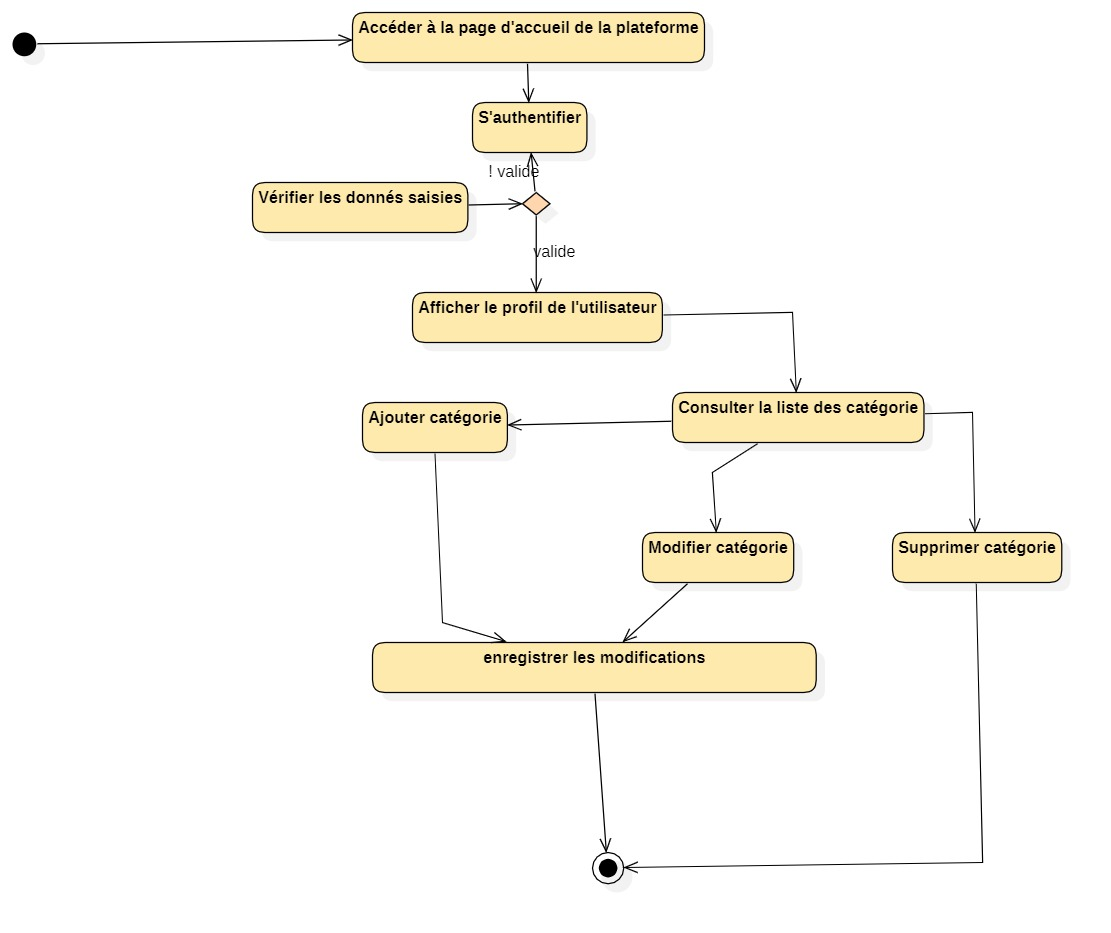
\includegraphics[width=14cm,height=13cm]{DiagrammeactivitésGérerfgzdfglescou.jpg}
	\caption{Diagramme d' activités « Gérer les catégories » .}
	\label{fig:Diagramme d' activités  Gérer les catégories  }
\end{figure}
\FloatBarrier

{\Large \color{cyan} Description des entités:}\\
La figure ci-dessus illustre le déroulement séquentiel de la gestion des accomplis par un Enseignant.\\
Après avoir s’authentifié, un Enseignant peut ajouter, modifier ou supprimer un catégorie.\\
Au cas d’ajout ou de modification du cours, le tuteur doit ajouter cet évènement  partagé pour informer les apprenants du changement.
\clearpage

%{+++++++++++++++++un autre section+++++++++++++++++++ }
%{+++++++++++++++++un autre section+++++++++++++++++++ }
%{+++++++++++++++++un autre section+++++++++++++++++++ }
%{+++++++++++++++++un autre section+++++++++++++++++++ }


%{+++++++++++++++++un autre section+++++++++++++++++++ }
%{+++++++++++++++++un autre section+++++++++++++++++++ }
%{+++++++++++++++++un autre section+++++++++++++++++++ }
%{+++++++++++++++++un autre section+++++++++++++++++++ }


\subsubsection{Les Interfaces de : gérer les catégories  }
Une fois authentifié,  l'enseignant peut accéder à son espace. \\ 
Il peut consulter la liste  des catégories comme la figure suivante
, comme il peut soit voir les catégories ou les modifier
via la liste affichée.  \\
Il peut aussi aussi ajouter un nouveau catégorie à partir de  la clique sur le bouton «ajouter un nouveau».  \\
à partir de cette clics la formulaire de la création d'un catégorie s'ouvre , il faut donc il faut que l'enseignant remplir le formulaire  pour créer un nouveau cours . \\
ci-dessous, illustrent ces opérations.
\medskip
\medskip
\medskip
\begin{figure}[ht]
	\centering
	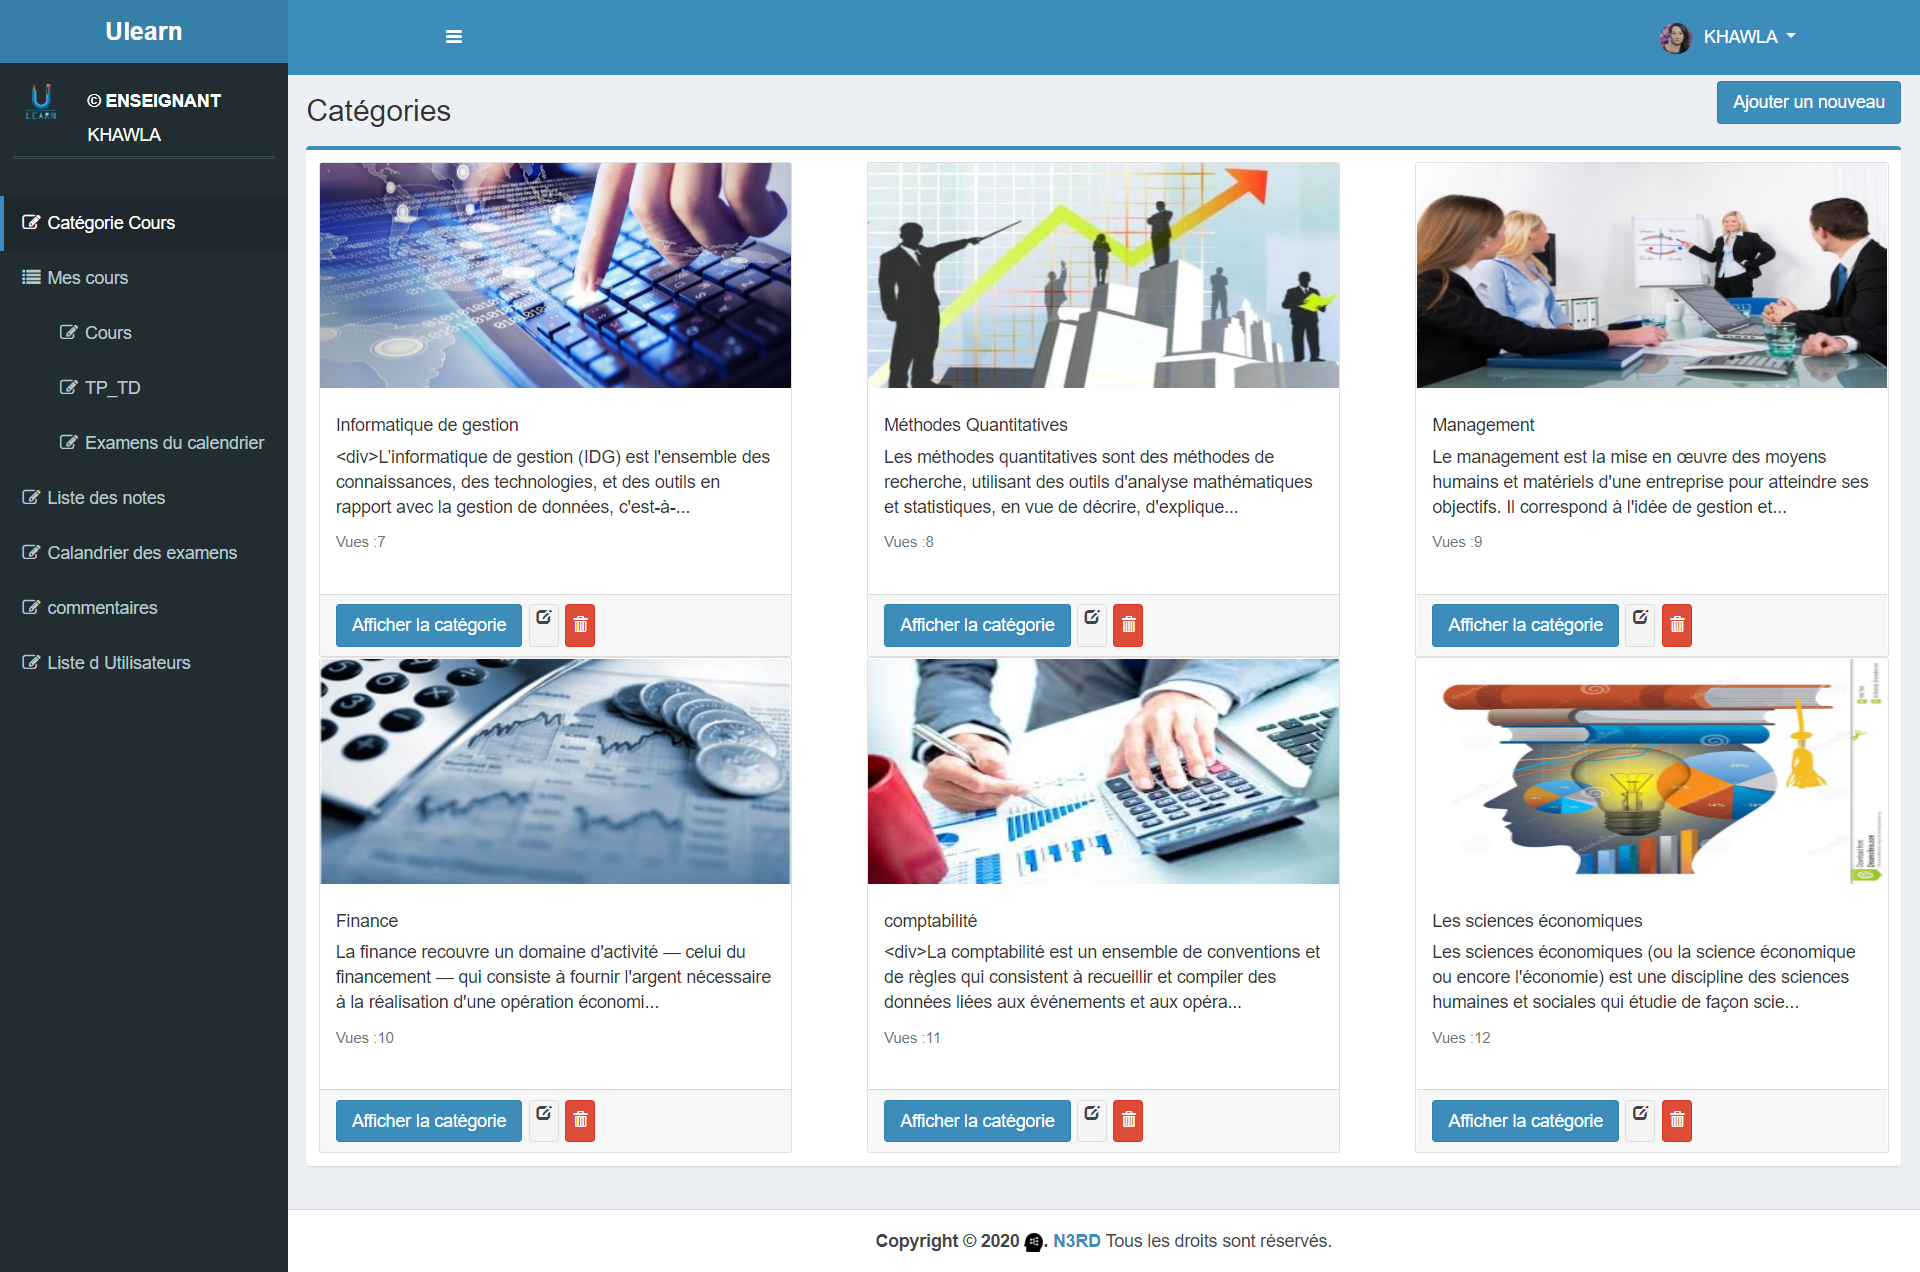
\includegraphics[width=15cm,height=13cm]{screencapture-localhost-8000-categories-2020-06-24-14_44_50.png}
	\caption{la liste des catégories .}
	\label{fig:la liste des catégories }
\end{figure}
\FloatBarrier

%{+++++++++++++++++un autre section+++++++++++++++++++ }
%{+++++++++++++++++un autre section+++++++++++++++++++ }
%{+++++++++++++++++un autre section+++++++++++++++++++ }
%{+++++++++++++++++un autre section+++++++++++++++++++ }

\begin{figure}[ht]
	\centering
	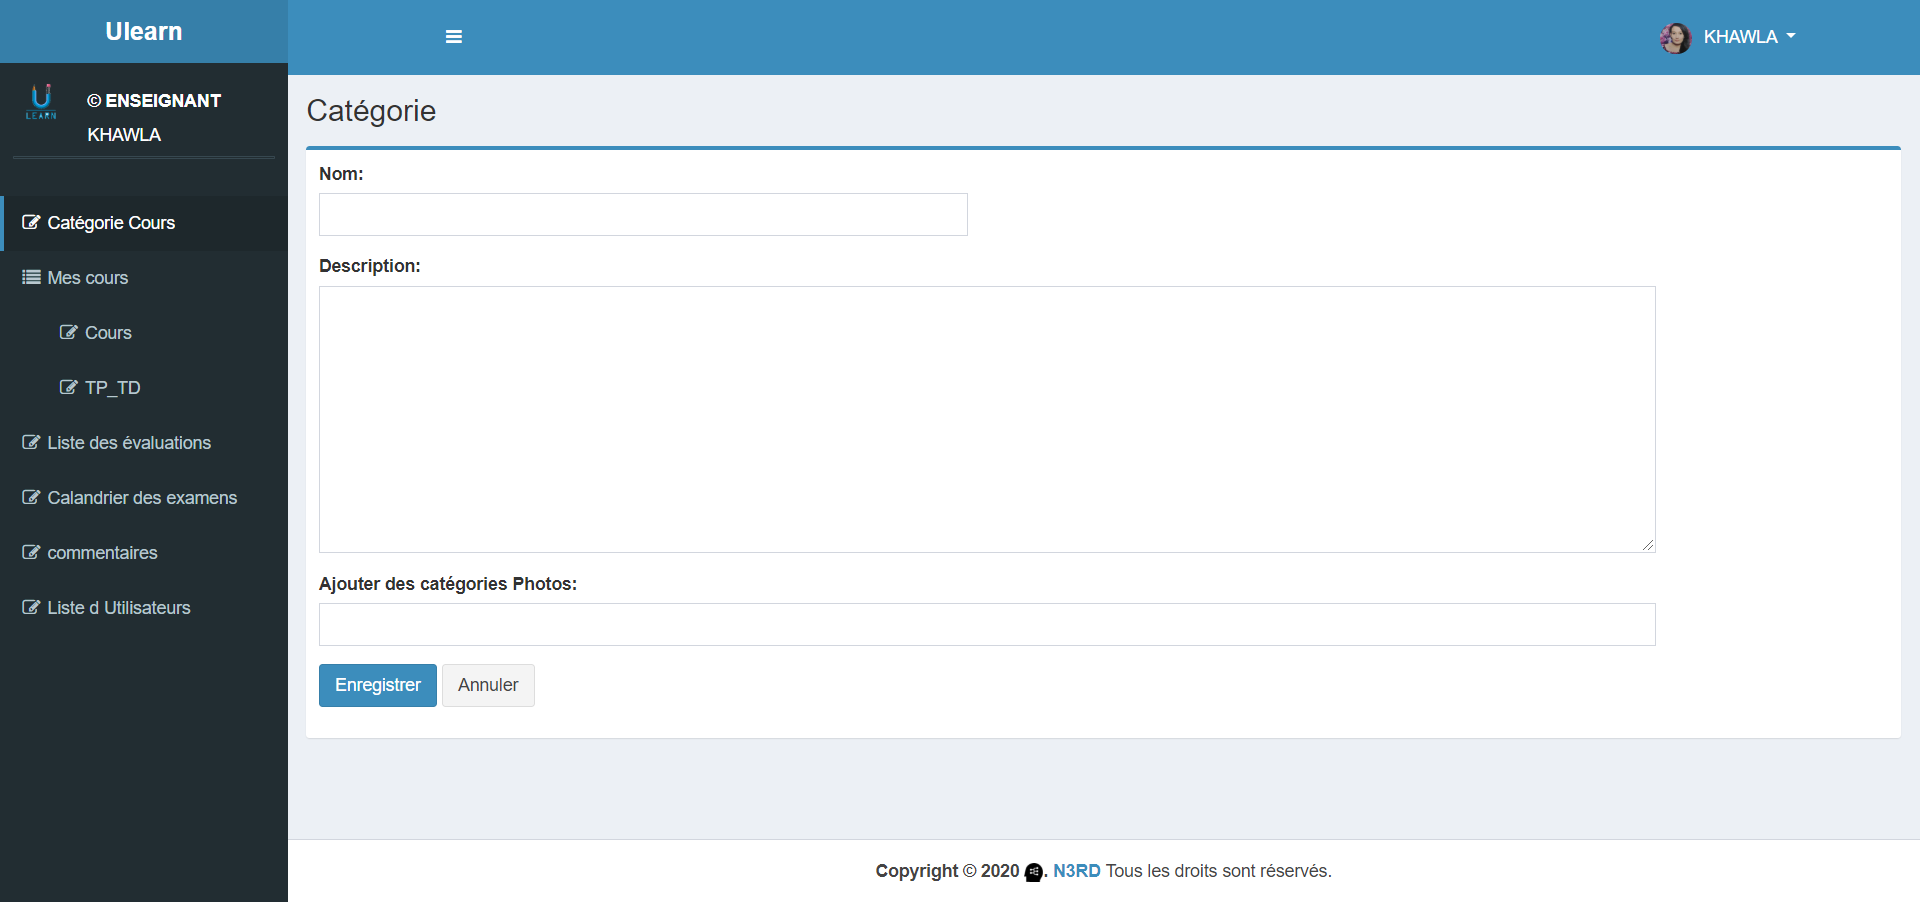
\includegraphics[width=15cm,height=9cm]{screencap.png}
	\caption{formulaire pour créer ou modifier un catégorie .}
	\label{fig: formulaire pour créer ou modifier un catégorie }
\end{figure}
\FloatBarrier
%{+++++++++++++++++un autre section+++++++++++++++++++ }
%{+++++++++++++++++un autre section+++++++++++++++++++ }
%{+++++++++++++++++un autre section+++++++++++++++++++ }
%{+++++++++++++++++un autre section+++++++++++++++++++ }

\begin{figure}[ht]
	\centering
	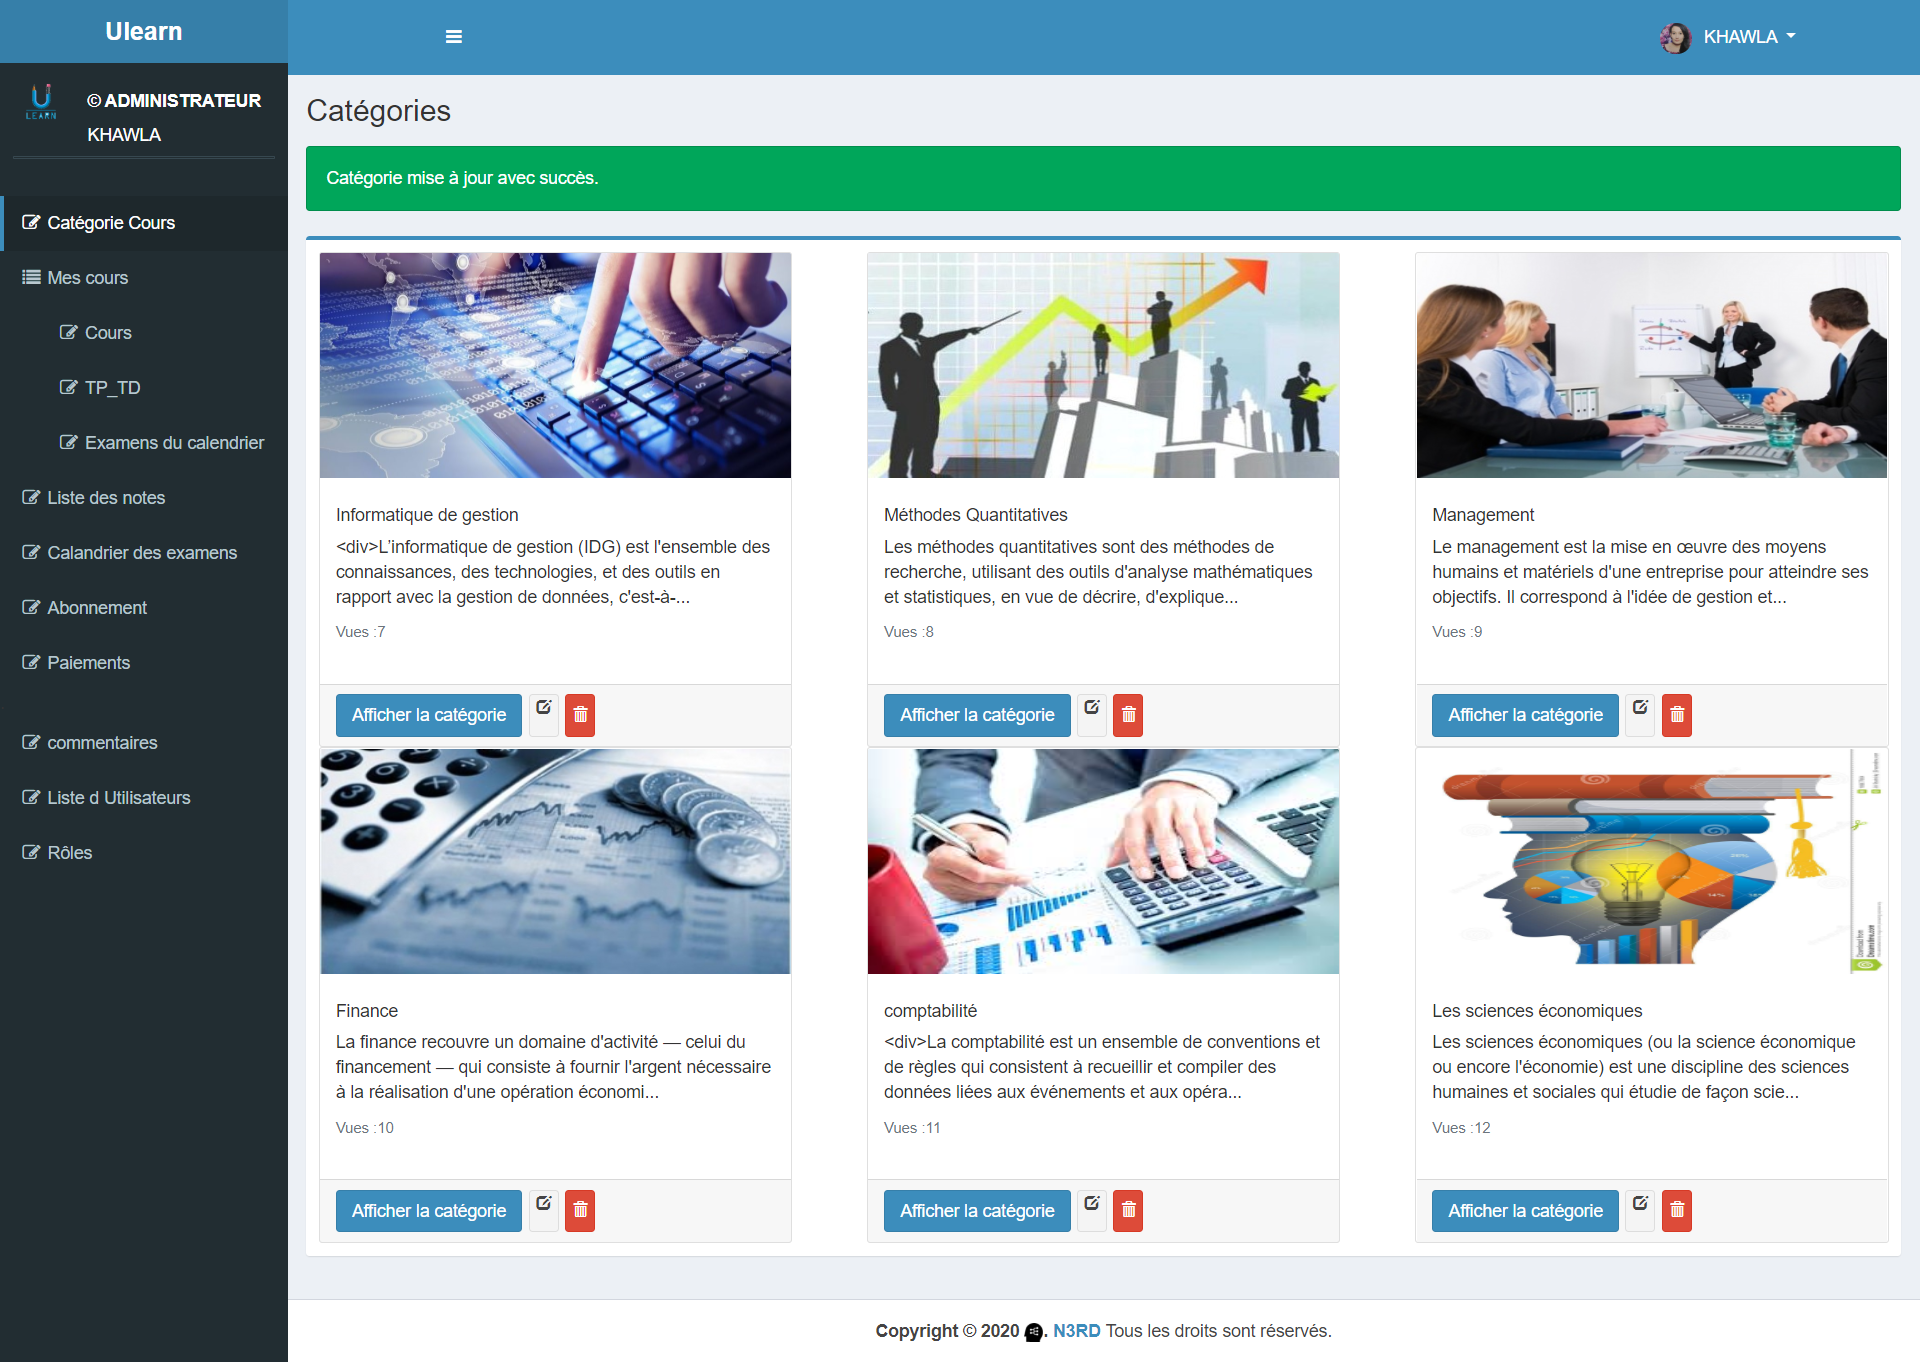
\includegraphics[width=15cm,height=9cm]{screencapture-localhost-8000-catnbnbegories-2020-06-24-22_20_06.png}
	\caption{Catégories avec quelques changements .}
	\label{fig: Catégories avec quelques changements  }
\end{figure}
\FloatBarrier



%{+++++++++++++++++un autre section+++++++++++++++++++ }
%{+++++++++++++++++un autre section+++++++++++++++++++ }
%{+++++++++++++++++un autre section+++++++++++++++++++ }
%{+++++++++++++++++un autre section+++++++++++++++++++ }
\clearpage

\subsection{item 2 : Gérer les  TD  -  TP}

\subsubsection{diagramme de séquences }
\begin{figure}[ht]
	\centering
	\includegraphics[width=13cm,height=10cm]{CasdutilisationGérerlestestslesexamens.jpg}
	\caption{Diagramme de Cas d' utilisation « Gérer les  TD  -  TP » .}
	\label{fig:Diagramme de Cas d' utilisation  Gérer les  TD  -  TP }
\end{figure}
\FloatBarrier
%{+++++++++++++++++un autre section+++++++++++++++++++ }
%{+++++++++++++++++un autre section+++++++++++++++++++ }
%{+++++++++++++++++un autre section+++++++++++++++++++ }
%{+++++++++++++++++un autre section+++++++++++++++++++ }
\subsubsubsection{Description détaillée des cas d’utilisations}
\begin{itemize}
	\item[$\bullet$] \textbf{Cas d’utilisation  Gérer les  TD  -  TP :} 
	\medskip
	\begin{itemize}
		\item \textit{\textbf{Objectif :}} permet à l’acteur d’ajouter, d’annuler et modifier les  TD  -  TP.
		\item \textit{\textbf{Acteur :}} Enseignants
		
		\item \textit{\textbf{Pré-condition  :}} L‘acteur doit être connecté.
		\item \textit{\textbf{Post-conditions   :}}
		\item \textit{\textbf{Scénario nominal :}}
		\begin{enumerate} 
			\item  l'enseignant saisir les informations de la formulaire TD  -  TP. 
			\item     l'enseignant configure les droits d’accès au test. 
			\item   l'enseignant enregistre informations .


		\end{enumerate}
	\end{itemize}
\end{itemize}	
\bigskip
\subsubsection{diagramme de séquences }
\begin{figure}[ht]
	\centering
	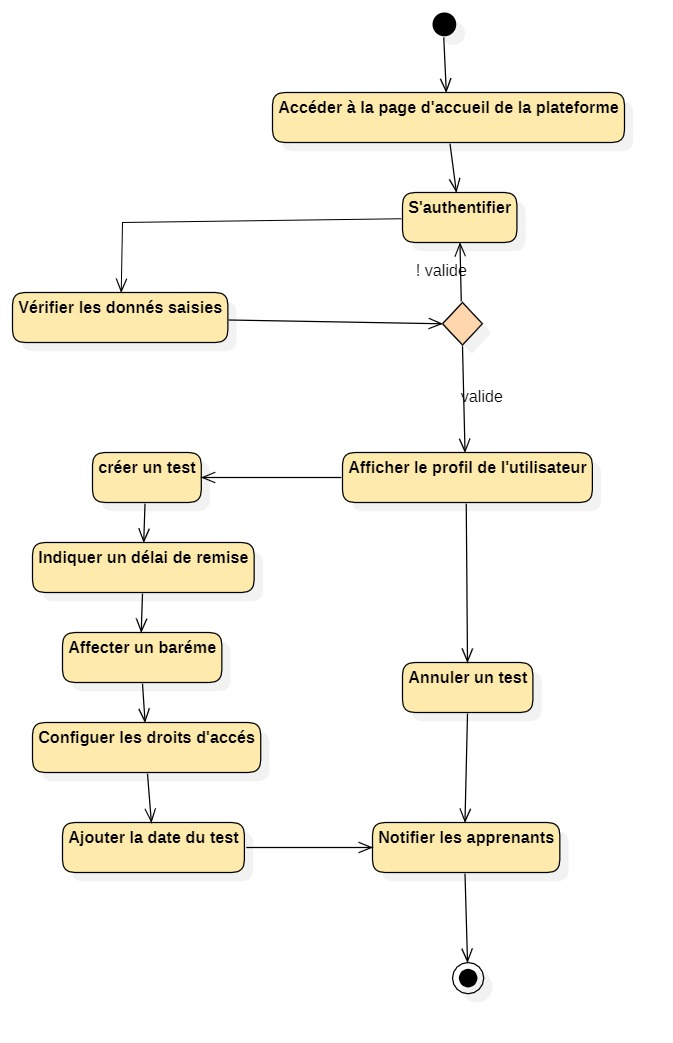
\includegraphics[width=13cm,height=13cm]{DiagrammeactivitésGérerlestestslesexamens.jpg}
	\caption{Diagramme d' activités « Gérer les  TD  -  TP » .}
	\label{fig:Diagramme d' activités  Gérer les  TD  -  TP }
\end{figure}
\FloatBarrier
{\Large \color{cyan} Description détaillée:}

La figure ci-dessus illustre le déroulement séquentiel de la gestion les  TD  -  TP accomplis par un
Enseignants.\\
Après l’authentification, un Enseignants peut ajouter ou annuler les  TD  -  TP. Au cas d’ajout, il faut lui
 remplir le formulaire  des informations de les  TD  -  TP.\\
Finalement, et c’est le cas d’annulation aussi, le tuteur doit sur le bouton Supprimer .
\clearpage


\subsubsection{Les Interfaces de :  Gérer les  TD  -  TP  }
Une fois authentifié,  l'enseignant peut accéder à son espace. \\ 
Il peut consulter la liste  les  TD  -  TP comme la figure suivante
, comme il peut soit voir les  TD  -  TP  supprimerou , modifier
 la liste affichée.  \\
Il peut aussi aussi ajouter un nouveau les  TD  -  TP à partir de  la clique sur le bouton «ajouter un nouveau».  \\
à partir de cette clics la formulaire de la création des les  TD  -  TP s'ouvre , il faut donc  l'enseignant remplir le formulaire  pour créer un nouveau les  TD  -  TP . \\
ci-dessous, illustrent ces opérations.
\medskip
\medskip
\medskip
\begin{figure}[ht]
	\centering
	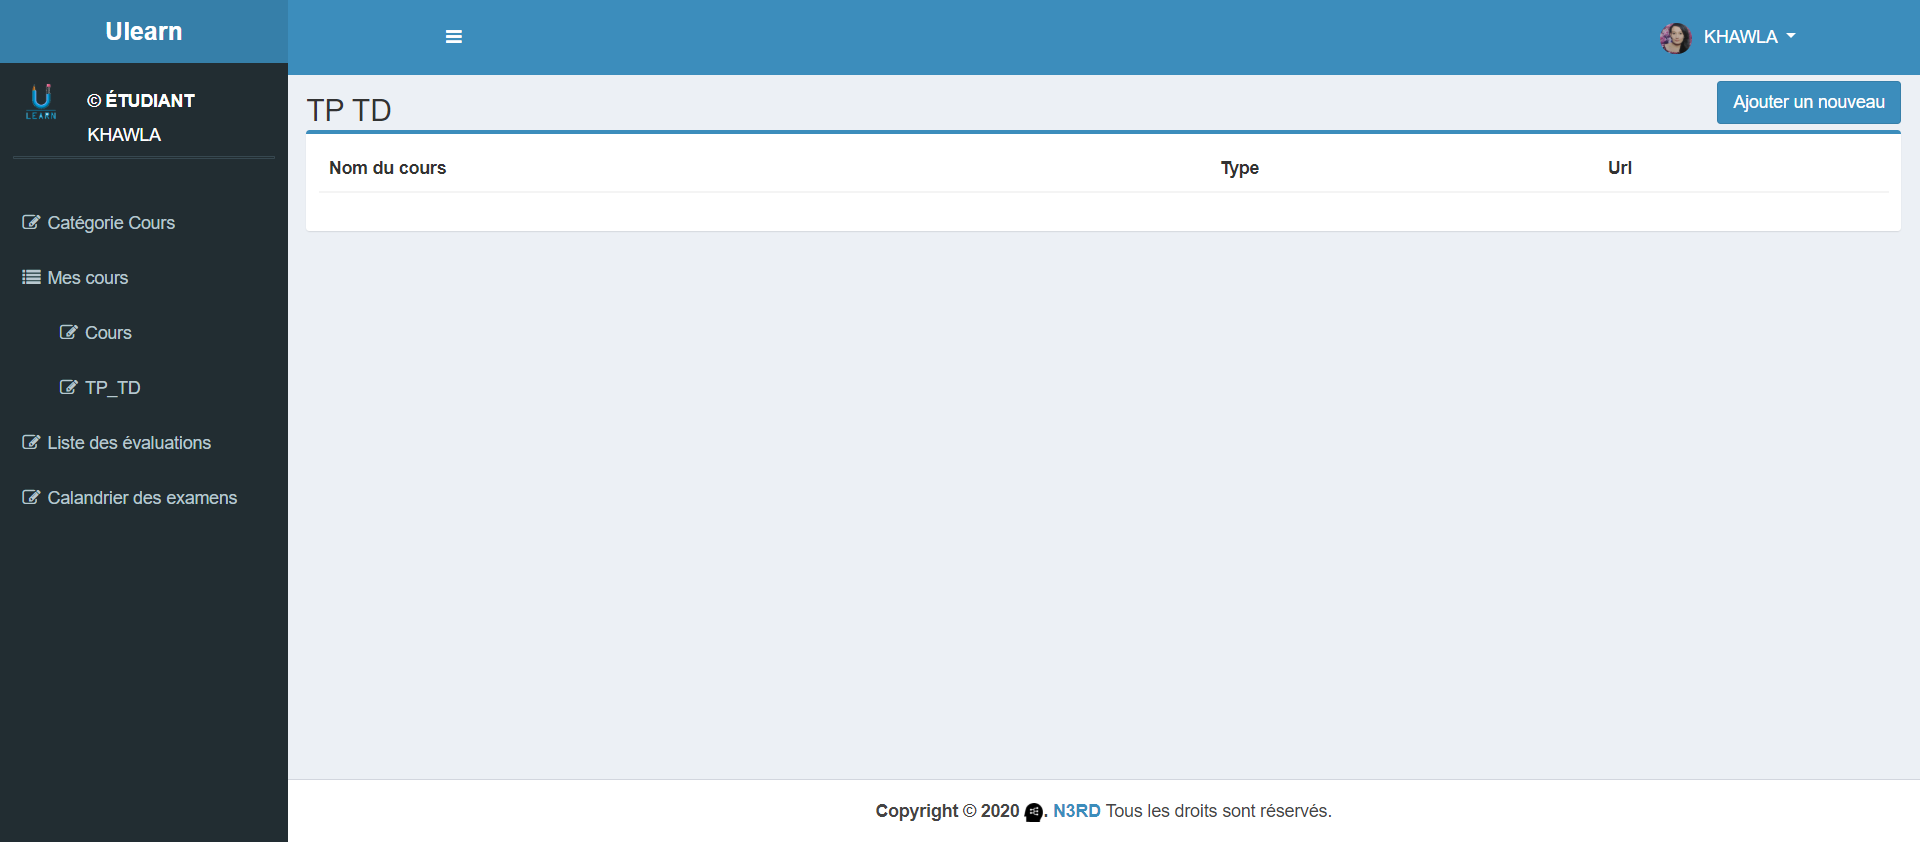
\includegraphics[width=15cm,height=13cm]{screencapture-localhost-9000-tpTds-2020-06-26-23_47_21.png}
	\caption{page d'évaluation.}
	\label{fig:page des TD  -  TP }
\end{figure}
\FloatBarrier
\clearpage
la figure ci-dessous représente la formulaire de la création des TD  -  TP
\begin{figure}[ht]
	\centering
	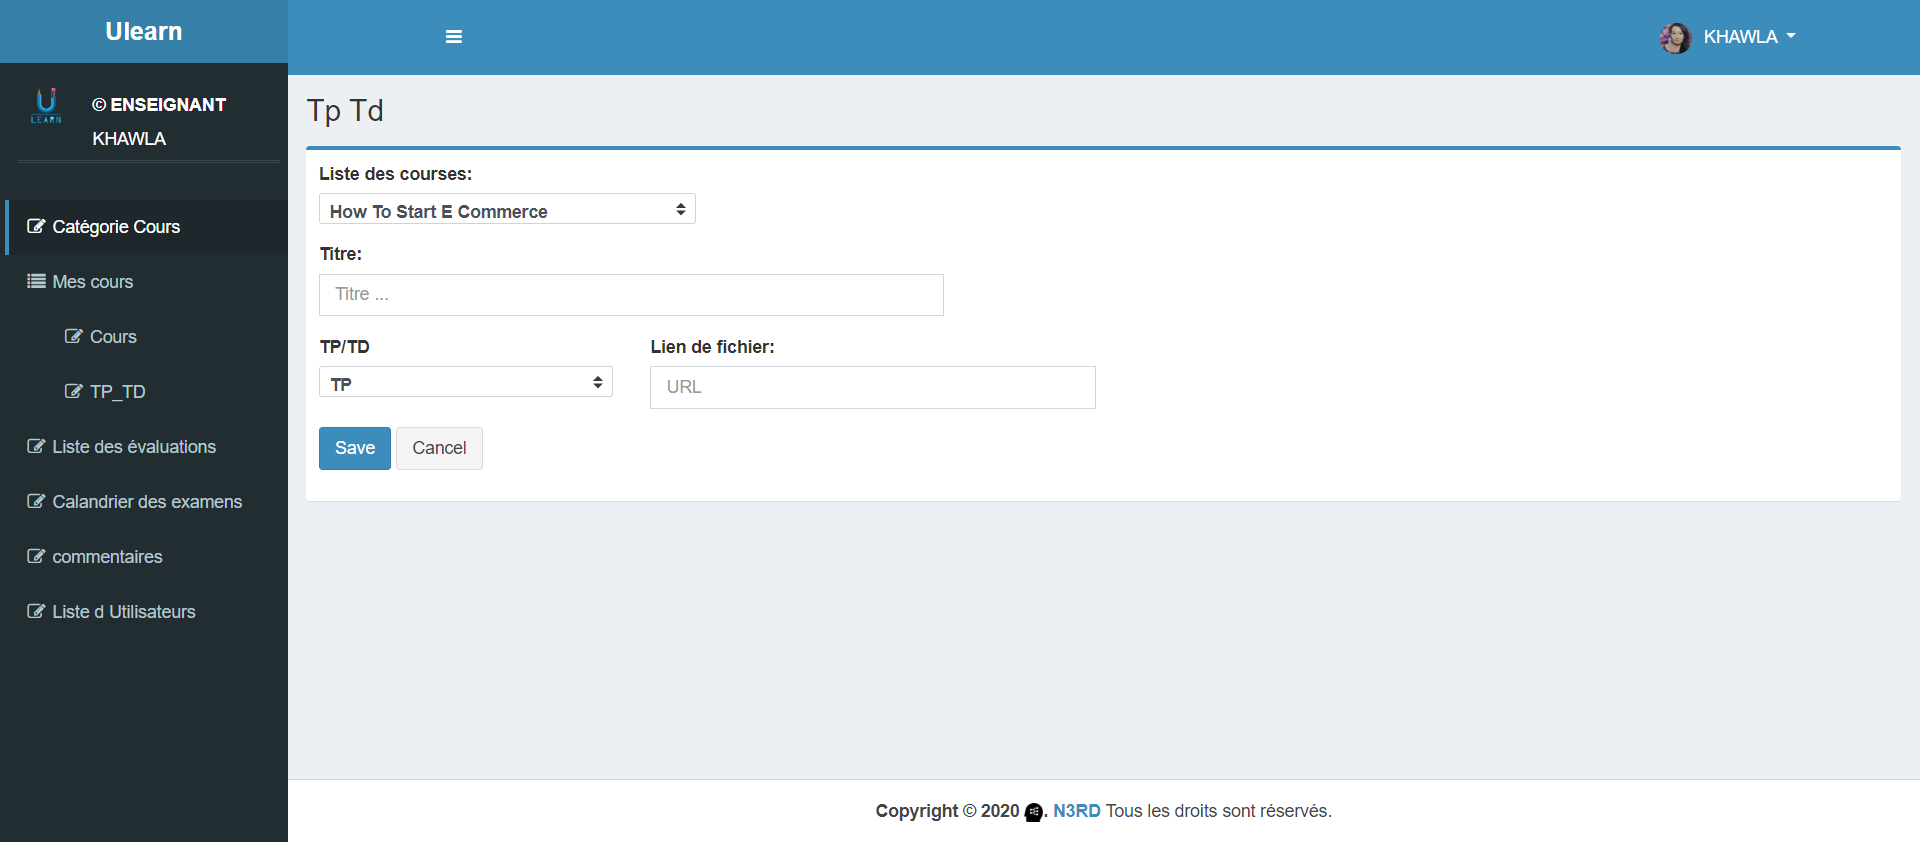
\includegraphics[width=15cm,height=8cm]{screencapture-localhost-9000-tpTds-create-2020-06-26-23_47_33.png}
	\caption{la formulaire de la création des TD  -  TP.}
	\label{fig:la formulaire de la création des TD  -  TP }
\end{figure}
\FloatBarrier
la figure ci-dessous représente la résultat de la création des TD  -  TP
\begin{figure}[ht]
	\centering
	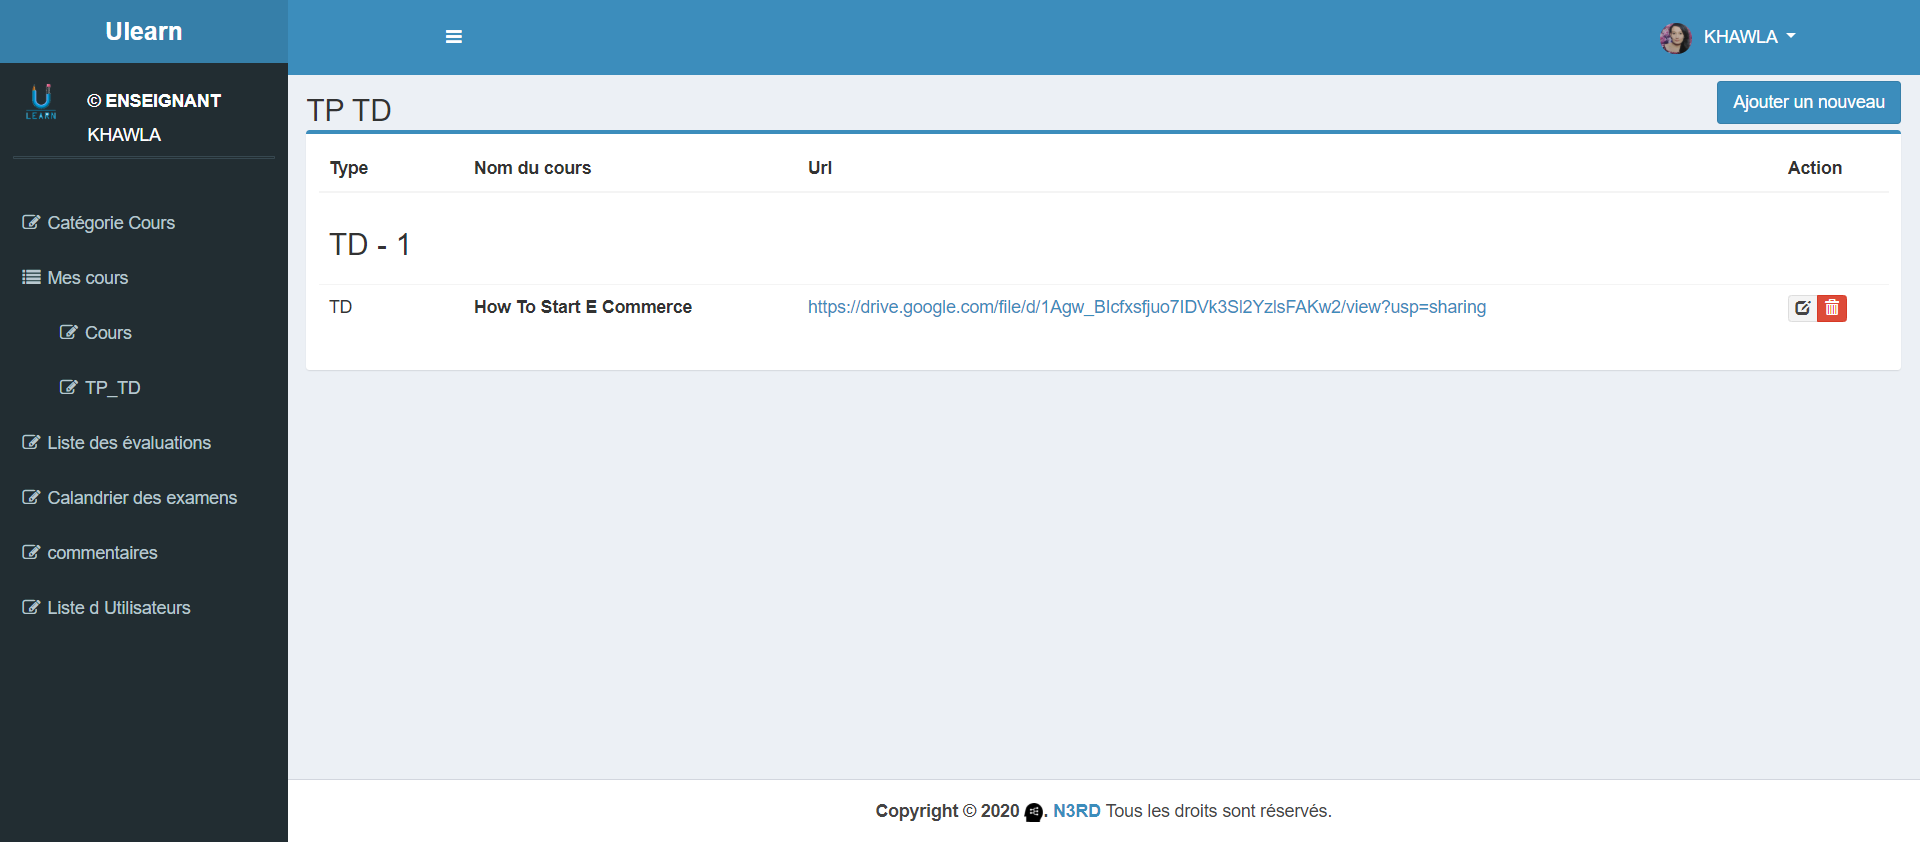
\includegraphics[width=15cm,height=6cm]{screencapture-localhost-9000-tpTds-2020-06-26-23_48_46.png}
	\caption{la résultat de la création des TD  -  TP.}
	\label{fig:la résultat de la création des TD  -  TP}
\end{figure}
\FloatBarrier
\clearpage
%{+++++++++++++++++un autre section+++++++++++++++++++ }
%{+++++++++++++++++un autre section+++++++++++++++++++ }
%{+++++++++++++++++un autre section+++++++++++++++++++ }
%{+++++++++++++++++un autre section+++++++++++++++++++ }
%{+++++++++++++++++un autre section+++++++++++++++++++ }
%{+++++++++++++++++un autre section+++++++++++++++++++ }
%{+++++++++++++++++un autre section+++++++++++++++++++ }
%{+++++++++++++++++un autre section+++++++++++++++++++ }
\subsection{item 3 : Gérer l'évaluation}
\subsubsection{Diagramme d' activités « d' affectation des notes étudiant » }
\begin{figure}[ht]
	\centering
	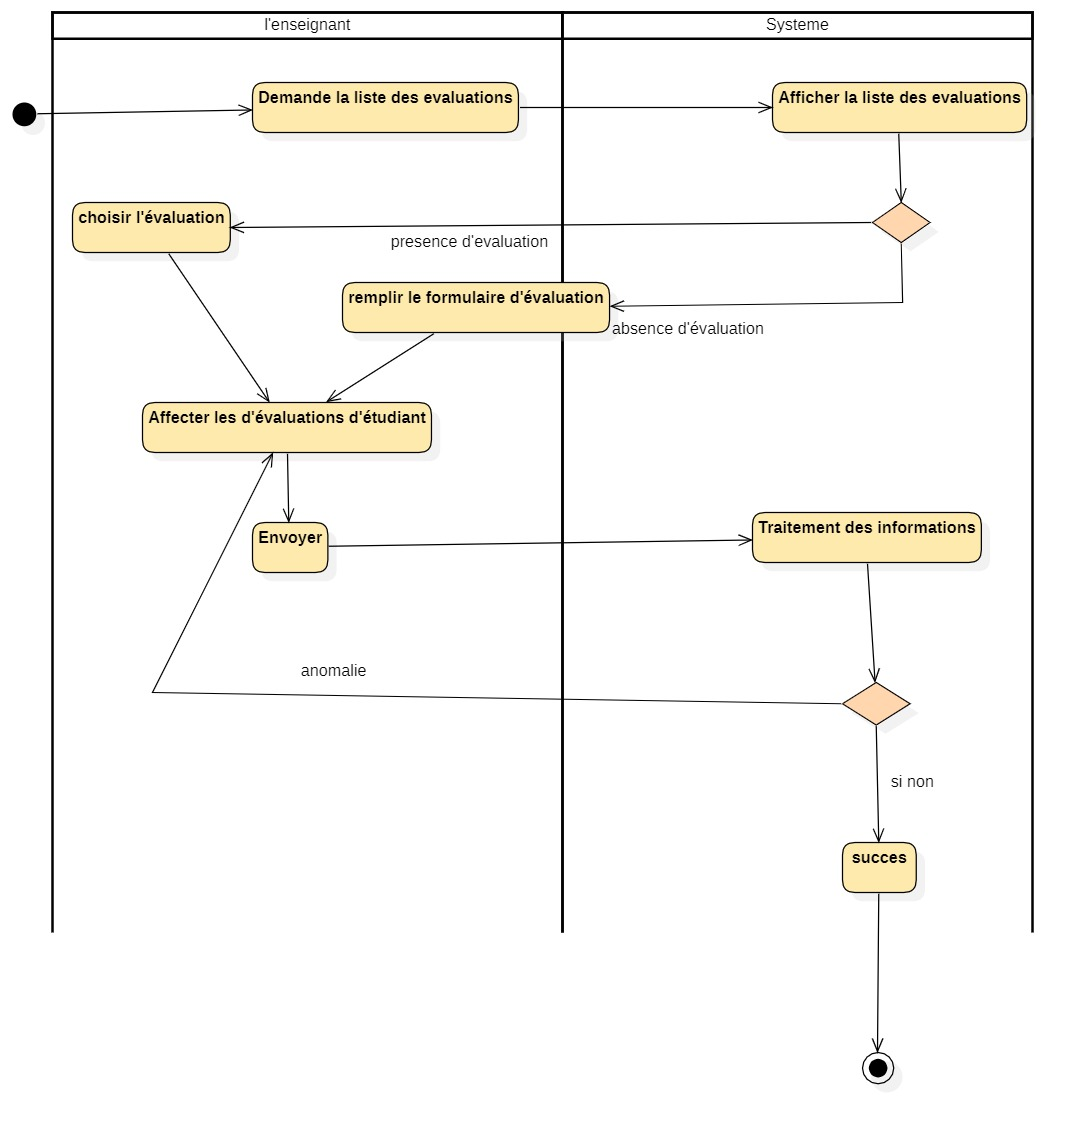
\includegraphics[width=13cm,height=10cm]{Diagrammedactivitésdaffectationdesnotesétudiant.jpg}
	\caption{Diagramme d' activités « d' affectation des notes étudiant » .}
	\label{fig:Diagramme d' activités  d' affectation des notes étudiant   }
\end{figure}
\FloatBarrier


{\Large \color{cyan} Description des entités :de diagramme d’activités «Affecter les notes d’élèves» }
\begin{itemize}	
	
	
	
	\item[$\star$]  l'enseignant demande la liste des évaluations.
	\item[$\star$] Le système affiche la liste des évaluations.
	\item[$\star$] En cas d’absence d’évaluation, l'enseignant doit créer l’évaluation.
	\item[$\star$] Si non, l'enseignant choisit l’évaluation et affecte l'URL des notes pour chaque  étudiant  à partir de la Google Drive.
	\item[$\star$] Puis envoyer les notes pour les sauvegarder.
	\item[$\star$] Le système traite les informations envoyées.
	\item[$\star$] En cas, d’une anomalie l’ajout est annulé.
	\item[$\star$] Si non, l’ajout est effectué avec succès.
	
	
	
%{+++++++++++++++++un autre section+++++++++++++++++++ }
%{+++++++++++++++++un autre section+++++++++++++++++++ }
%{+++++++++++++++++un autre section+++++++++++++++++++ }
%{+++++++++++++++++un autre section+++++++++++++++++++ }
%{+++++++++++++++++un autre section+++++++++++++++++++ }
%{+++++++++++++++++un autre section+++++++++++++++++++ }
%{+++++++++++++++++un autre section+++++++++++++++++++ }
%{+++++++++++++++++un autre section+++++++++++++++++++ }

\subsubsection{Les Interfaces de : gérer l'évaluation  }
Une fois authentifié,  l'enseignant peut accéder à son espace. \\ 
Il peut consulter la liste  des évaluations comme la figure suivante
, comme il peut soit voir les catégories  supprimerou les modifier
via la liste affichée.  \\
Il peut aussi aussi ajouter un nouveau d'évaluation à partir de  la clique sur le bouton «ajouter un nouveau».  \\
à partir de cette clics la formulaire de la création d'évaluation s'ouvre , il faut donc  l'enseignant remplir le formulaire  pour créer un nouveau 'évaluation . \\
ci-dessous, illustrent ces opérations.
\medskip
\medskip
\medskip
\begin{figure}[ht]
	\centering
	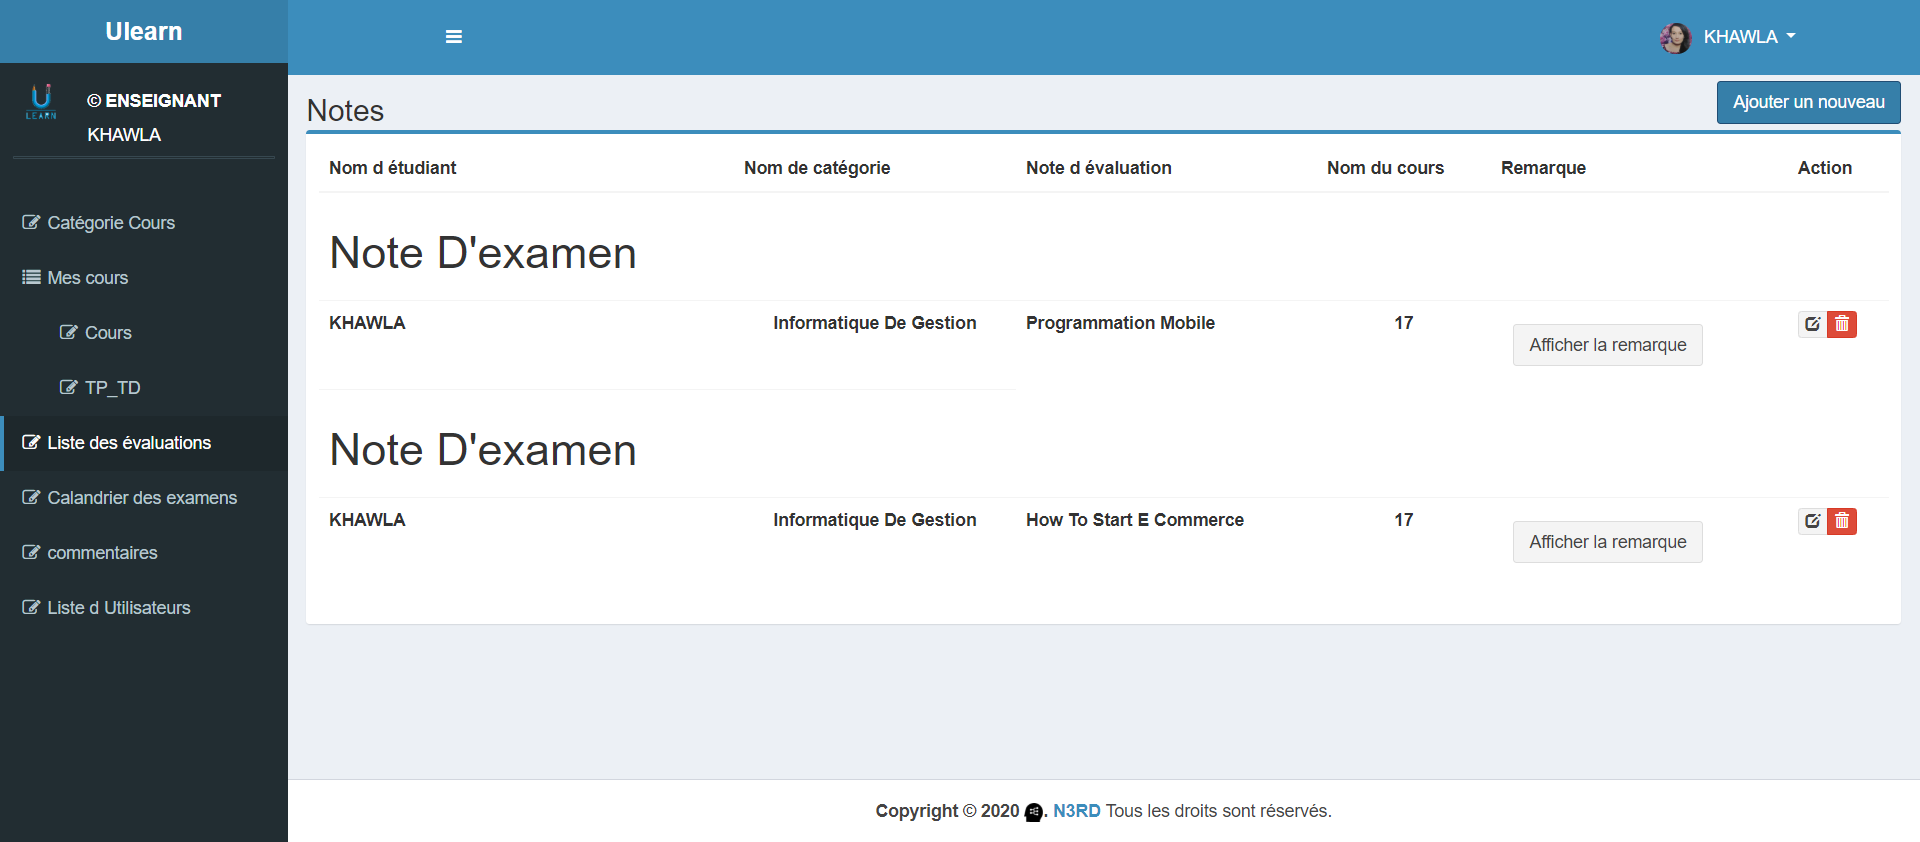
\includegraphics[width=15cm,height=13cm]{screencapture-localhost-9000-notes-2020-06-26-23_11_18.png}
	\caption{page d'évaluation.}
	\label{fig:page d'évaluation }
\end{figure}
\FloatBarrier
\begin{figure}[ht]
	\centering
	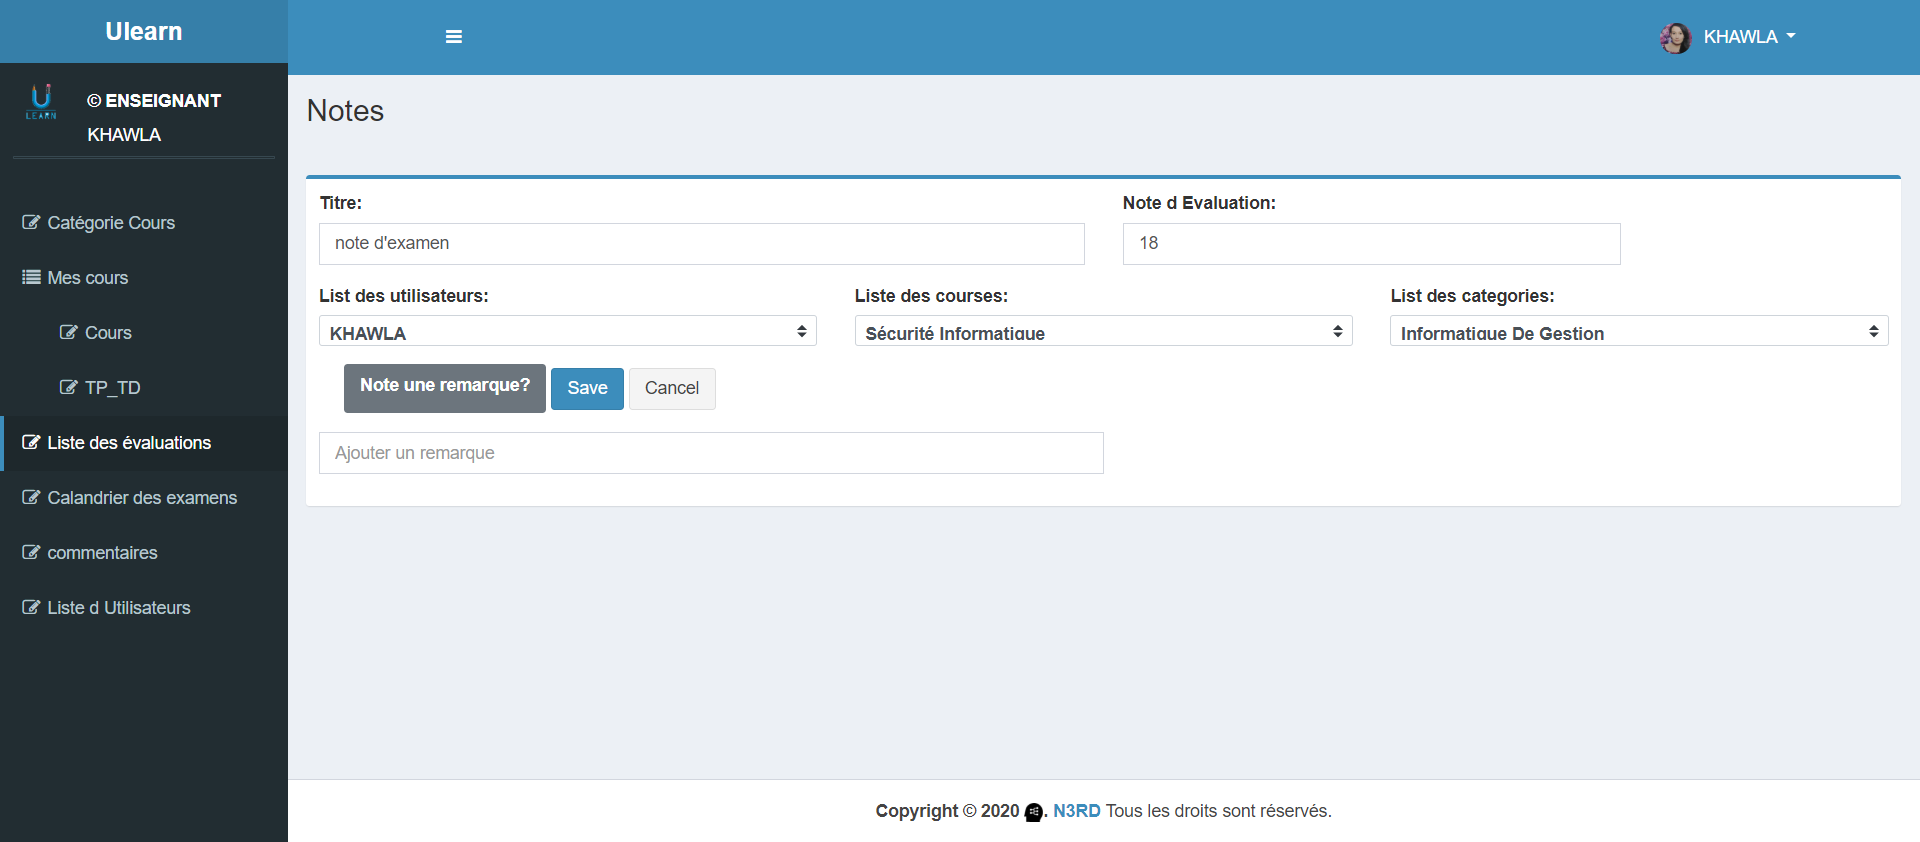
\includegraphics[width=15cm,height=7cm]{screencapture-localhost-9000-notes-create-2020-06-26-23_13_54.png}
	\caption{formulaire d'évaluation .}
	\label{fig:formulaire d'évaluation }
\end{figure}
\FloatBarrier
la figure ci-dessous représente la résultat  d'enregistrement d'évaluation de côtés enseignant .
\begin{figure}[ht]
	\centering
	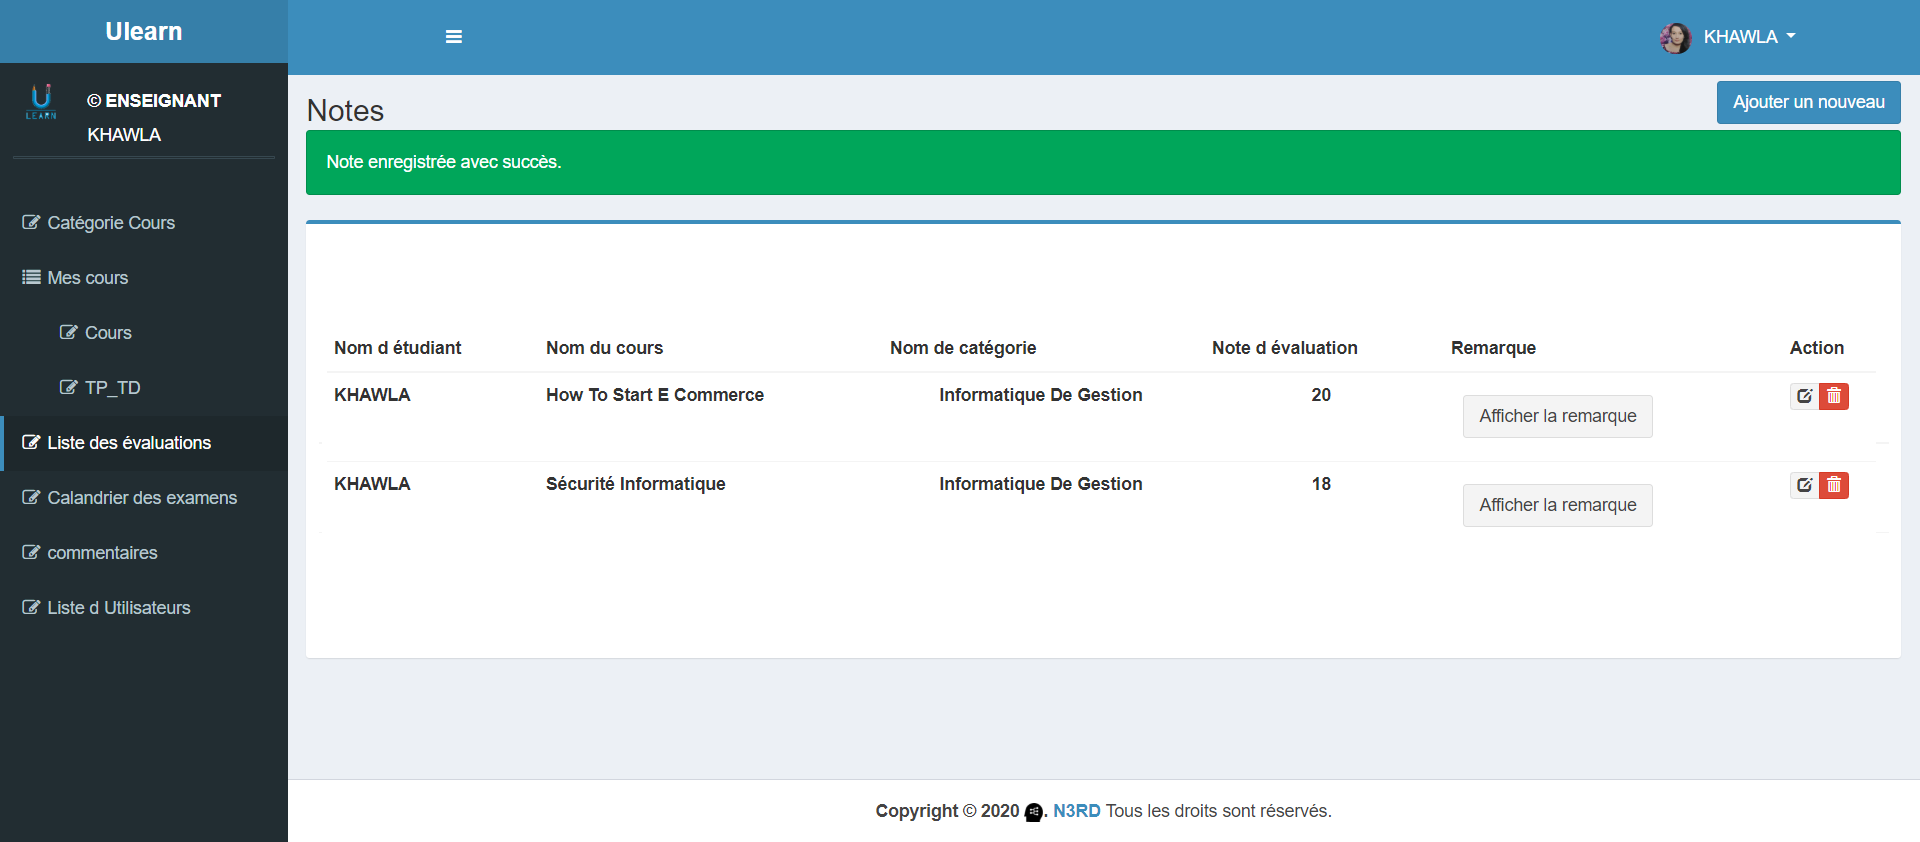
\includegraphics[width=15cm,height=7.4cm]{screencapture-localhost-9000-notes-2020-06-26-23_15_22.png}
	\caption{résultat d'évaluation.}
	\label{fig:résultat d'évaluation }
\end{figure}
\FloatBarrier
\clearpage
	
\end{itemize}


\clearpage
\section{Sprint 4 : Étudiant}
\label{sec:conception}

\begin{fquote}
	Ce premier sprint s’étale sur 11 jours et se décompose en 2 items
\end{fquote}
\smallskip
\begin{itemize}[label=$\diamond$]
	\item Consulter les ressources et les liens d'apprentissage
	
	\item consulter calendrier , consulter l'évaluation
 
	
\end{itemize}
\medskip
\medskip
\medskip
\medskip
\medskip
\medskip
\medskip
\medskip
\medskip
\medskip
\begin{figure}[ht]
	\centering
	\includegraphics[width=13cm,height=10cm]{Décompositionsprint4enItems.png}
	\caption{Décomposition sprint 4 en Items.}
	\label{fig:Démposition sprint 4 en Items}
\end{figure}
\FloatBarrier
\clearpage

%{+++++++++++++++++un autre section+++++++++++++++++++ }
%{+++++++++++++++++un autre section+++++++++++++++++++ }
%{+++++++++++++++++un autre section+++++++++++++++++++ }
%{+++++++++++++++++un autre section+++++++++++++++++++ }

\begin{table}[]
	{\Large\color{cyan} Le backlog du sprint 4 est le suivant :}\\
	
	\begin{tabular}{|l|l|l|l|}
		\hline 
		\rowcolor{-blue!20!red}{Item}                         & \textbf{User Story}                                                   & \textbf{Description}                                                                                              & \textbf{Priorité} \\ \hline
		\begin{tabular}[c]{@{}l@{}}\textbf{Consulter  }\\ \textbf{les ressources  }\\ \textbf{ et les liens }\\ \textbf{d'apprentissage } \end{tabular}                    &        \begin{tabular}[c]{@{}l@{}}Consulter  \\ les ressources \\  et les liens \\ d'apprentissage  \end{tabular}                                                    & \begin{tabular}[c]{@{}l@{}}En tant qu'étudiant, je peux \\consulter la liste des catégories \\et puis je peux choisir un cours \\et je dois  le paye pour le suivre  \end{tabular}                                                                         & 1    \\ \hline
			\begin{tabular}[c]{@{}l@{}}\textbf{Consulter  }\\ \textbf{le calendrier ,}\\ \textbf{et consulter}\\ \textbf{l'évaluation} \end{tabular}                & \begin{tabular}[c]{@{}l@{}}Consulter  \\ le calendrier  \end{tabular}                                                       & \begin{tabular}[c]{@{}l@{}}En tant qu'un étudiant\\  je peux
				afficher le calendrier\\et je peux consulter mes notes\end{tabular} & 2                 \\ \hline
	\end{tabular}
	\caption{Tables Backlog du sprint 4}
	\label{Tables Backlog du sprint 4}
\end{table}
\begin{table}[h]
%{+++++++++++++++++un autre section+++++++++++++++++++ }
%{+++++++++++++++++un autre section+++++++++++++++++++ }
%{+++++++++++++++++un autre section+++++++++++++++++++ }
%{+++++++++++++++++un autre section+++++++++++++++++++ }	
	
	 
	
%{+++++++++++++++++un autre section+++++++++++++++++++ }
%{+++++++++++++++++un autre section+++++++++++++++++++ }
%{+++++++++++++++++un autre section+++++++++++++++++++ }
%{+++++++++++++++++un autre section+++++++++++++++++++ }	
	{\Large \color{cyan} les user stories de sprint 4:}
	
	\begin{center}
		\begin{tabular}{>{\begin{bf} } c <{\end{bf}}ccc}
			
			\rowcolor{-blue!20!red}ID U.S & \begin{bf}User Story \end{bf}  & \\
			
			1 &en tant que étudiant je peux parcourir \\
			&la liste  des catégories et puis je peux choisir \\
			&un cours dans la liste des cours ou à partir de la catégorie\\
			& choisir et pour accéder à la cours il faut tout d'abord\\
			& payer les frais d'abonnement
			\\
			& \\
			2 & En tant qu'un étudiant je peux choisir l'option
			calendrier \\ & et je peux consulter les notes	\\
		
			
		\end{tabular}
	\end{center}
	\caption{Tables  "les user stories de sprint 4"}
	\label{les user stories de sprint 4}
\end{table}



\clearpage
\clearpage
\subsection{item 1 : Consulter les ressources et les liens d'apprentissage}
\subsubsection{Diagramme de cas d’utilisation  détaillé «Étudiant» }
L’image suivante présente le diagramme de cas d’utilisation détaillé «Étudiant»
\begin{figure}[ht]
	\centering
	\includegraphics[width=17cm,height=10cm]{DiagrammedecasdutilisationdétailléÉtudiant.jpg}
	\caption{Diagramme de cas d' utilisation  détaillé «Étudiant» .}
	\label{fig:Diagramme de cas d' utilisation  détaillé Étudiant  }
\end{figure}
\FloatBarrier
{\Large \color{cyan} Description détaillée:}

Description textuelle de cas d’utilisation « Consulter la liste des cours fermé (privé)».


\begin{itemize}
	
	\item[$\bullet$] \textbf{Consulter la liste des cours :} permet à l’acteur de Consulter la liste des cours et
	 accéder à un cours
	\begin{itemize}
		\item \textit{\textbf{Objectif :}}  Permettre à l'étudiant de consulter la liste des catégories et la liste des cours et acceder a un cours privé (fermé) apres paiement . 
		
		\item \textit{\textbf{Acteur :}} Tous les étudiants
		
		\item \textit{\textbf{Pré-condition  :}}  L'étudiant s’authentifie.

		\item \textit{\textbf{Scénario nominal :}}
		\begin{enumerate}
			\item L’utilisateur accède à la page d’accueil de E-Learning.
\item L'utilisateur accède à la liste des catégories
\item L'utilisateur choisit un catégorie
\item L'utilisateur accède à la liste des cours privés.
\item L’utilisateur clique sur l’un des liens de cours privés.
\item L'utilisateur achète les cours
\item Le système donner l'accès de l'utilisateur  a la cours
\item Le système visualise le cours selon le format (Vidéo ,PDF…etc).
		\end{enumerate}
		\item \textit{\textbf{Scénario alternative :}} \\
		les informations sont manquantes ou incorrectes: ce scénario commence au point 04 du
		scénario nominal.
		\begin{enumerate}
			
			\item L'étudiant n'est pas réussi a l'achat , le système affiche un
			message d’erreur et revient à l’étape 4 de scénario nominal. nominal. 
		\end{enumerate}
	\end{itemize}
\end{itemize}	
\bigskip



\subsubsection{diagramme de séquences }
La figure  ci-dessous représente le diagramme de séquence: consulter les ressources et les liens d' apprentissage .

\begin{figure}[ht]
	\centering
	\includegraphics[width=13cm,height=7cm]{dliensapprentissage.jpg}
	\caption{Diagramme de séquence: consulter les ressources et les liens d' apprentissage .}
	\label{fig:diagramme de séquence: consulter les ressources et les liens d' apprentissage }
\end{figure}
\FloatBarrier

Ce diagramme de séquence illustre l’échange entre l'apprenant et le système  donc Pour consulter les ressources et les liens d' apprentissage, un apprenant doit demander la liste des ressources et liens , le systeme charger la page des ressources et liens  (categores , cours , tp et td) .

%{+++++++++++++++++un autre section+++++++++++++++++++ }
%{+++++++++++++++++un autre section+++++++++++++++++++ }
%{+++++++++++++++++un autre section+++++++++++++++++++ }
%{+++++++++++++++++un autre section+++++++++++++++++++ }
\subsubsection{Les Interfaces de : Consulter les ressources et les liens d'apprentissage  }

la figure ci-dessous représente l'interface de la liste des catégories donc à partir de cela l'étudiant peut  parcourir et reconnaît les différents catégories .
\begin{figure}[ht]
	\centering
	\includegraphics[width=17cm,height=7cm]{eyjgkjo.png}
	\caption{Interface : la liste des catégories .}
	\label{fig:Interface : la liste des catégories }
\end{figure}
\FloatBarrier
%{+++++++++++++++++un autre section+++++++++++++++++++ }
%{+++++++++++++++++un autre section+++++++++++++++++++ }
%{+++++++++++++++++un autre section+++++++++++++++++++ }
%{+++++++++++++++++un autre section+++++++++++++++++++ }
\bigskip
\bigskip
\bigskip
la figure ci-dessous représente les différents détails de la catégorie et les différents cours qui appartient à cette catégorie  , donc à partir de la catégorie on peut passer à la cours choisir .
\begin{figure}[ht]
	\centering
	\includegraphics[width=17cm,height=6cm]{eyooogkjo.png}
	\caption{Interface : détail d'une catégorie .}
	\label{fig:Interface : détail d'une catégorie }
\end{figure}
\FloatBarrier
%{+++++++++++++++++un autre section+++++++++++++++++++ }
%{+++++++++++++++++un autre section+++++++++++++++++++ }
%{+++++++++++++++++un autre section+++++++++++++++++++ }
%{+++++++++++++++++un autre section+++++++++++++++++++ }
\clearpage
la figure ci-dessous représente l'interface qui permet à l'étudiant de choisir et rejoindre un cours .

\medskip

Comme  il peut aussi regarder les Vidéos d'introduction à la courset comment la créateur de la cours .
\bigskip
\bigskip
\bigskip
\begin{figure}[ht]
	\centering
	\includegraphics[width=17cm,height=11cm]{qgbmb.png}
	\caption{Interface : la liste des cours .}
	\label{fig:Interface : la liste des cours }
\end{figure}
\FloatBarrier
%{+++++++++++++++++un autre section+++++++++++++++++++ }
%{+++++++++++++++++un autre section+++++++++++++++++++ }
%{+++++++++++++++++un autre section+++++++++++++++++++ }
%{+++++++++++++++++un autre section+++++++++++++++++++ }
\bigskip
\bigskip
\bigskip
Une fois l'étudiant accéder  à ce interface  après avoir appuyé sur le bouton dans le Figure précédentepleut il peut consulter les différents détails de la cours .

\medskip

 Comme il peut soit regarder les Vidéos d'introduction à la cours ou poser des questions sous forme des commentaires  ou bien payer les frais d'abonnement .
\begin{figure}[ht]
	\centering
	\includegraphics[width=17cm,height=20cm]{screencapture-127-0-0-1-8000-courses-12-2020-06-22-12_20_28.png}
	\caption{Interface : un cours avant paiement .}
	\label{fig:Interface :un cours avant paiement }
\end{figure}
\FloatBarrier
%{+++++++++++++++++un autre section+++++++++++++++++++ }
%{+++++++++++++++++un autre section+++++++++++++++++++ }
%{+++++++++++++++++un autre section+++++++++++++++++++ }
%{+++++++++++++++++un autre section+++++++++++++++++++ }
Paystack offre un interface de test gratuite pour leurs utilisateurs
donc l'étudiant après passer par la figure précédente , le système ouvre automatiquement cette interface de payement .
\begin{figure}[ht]
	\centering
	\includegraphics[width=17cm,height=14cm]{mimi.png}
	\caption{Interface : la plateforme de test  paystack .}
	\label{fig:Interface : la plateforme de test  paystack }
\end{figure}
\FloatBarrier
%{+++++++++++++++++un autre section+++++++++++++++++++ }
%{+++++++++++++++++un autre section+++++++++++++++++++ }
%{+++++++++++++++++un autre section+++++++++++++++++++ }
%{+++++++++++++++++un autre section+++++++++++++++++++ }
la figure ci-dessous représente un cours déjà payé avec des nouveaux d'options .
\begin{figure}[ht]
	\centering
	\includegraphics[width=17cm,height=20cm]{screencapture-localfhdhost-8000-courses-10-2020-06-22-12_43_22.png}
	\caption{Interface : un cours après paiement .}
	\label{fig:Interface :un cours après paiement }
\end{figure}
\FloatBarrier






%{+++++++++++++++++un autre section+++++++++++++++++++ }
%{+++++++++++++++++un autre section+++++++++++++++++++ }
%{+++++++++++++++++un autre section+++++++++++++++++++ }
%{+++++++++++++++++un autre section+++++++++++++++++++ }

\clearpage
\subsection{item 2 : consulter calendrier , consulter l'évaluation }
\subsubsection{diagramme de séquences : consulter calendrier }
La figure  ci-dessous représente le diagramme de séquences consulter agenda pour un  étudiant.

\begin{figure}[ht]
	\centering
	\includegraphics[width=13cm,height=4cm]{diagrammedeséquencesconsulteragendadeslivrable.jpg}
	\caption{Diagramme de séquences consulter le calendrier  .}
	\label{fig:Diagramme de séquences consulter le calendrier }
\end{figure}
\FloatBarrier

Ce diagramme de séquence illustre l'interaction entre l'apprenant et le système afin de consulter le
calendrier donc  Pour consulter calendrier, un apprenant doit  demander calendrier , puis le systeme charger calendrier .
%{+++++++++++++++++un autre section+++++++++++++++++++ }
%{+++++++++++++++++un autre section+++++++++++++++++++ }
%{+++++++++++++++++un autre section+++++++++++++++++++ }
%{+++++++++++++++++un autre section+++++++++++++++++++ }

\subsubsection{diagramme de séquences : consulter l'évaluation }
La figure  ci-dessous représente le diagramme de séquences de consulter l'évaluation  pour un  étudiant.

\begin{figure}[ht]
	\centering
	\includegraphics[width=13cm,height=4cm]{rfbhdtjlivrables.jpg}
	\caption{Diagramme de séquences consulter l'évaluation   .}
	\label{fig:Diagramme de séquences consulter l'évaluation  }
\end{figure}
\FloatBarrier

Ce diagramme de séquence illustre l'interaction entre l'apprenant et le système afin de consulter l'évaluation  donc  Pour consulter l'évaluation, un apprenant doit  demander l'évaluation , puis le systeme charger l'évaluation .



\clearpage
%{+++++++++++++++++un autre section+++++++++++++++++++ }
%{+++++++++++++++++un autre section+++++++++++++++++++ }
%{+++++++++++++++++un autre section+++++++++++++++++++ }
%{+++++++++++++++++un autre section+++++++++++++++++++ }

%{+++++++++++++++++un autre section+++++++++++++++++++ }
%{+++++++++++++++++un autre section+++++++++++++++++++ }
%{+++++++++++++++++un autre section+++++++++++++++++++ }
%{+++++++++++++++++un autre section+++++++++++++++++++ }

\subsection{Diagramme d' activité: d' un apprenant sur l' espace}


\begin{figure}[ht]
	\centering
	\includegraphics[width=15cm,height=16cm]{Diagrammedactivitédunapprenantsurlespace.jpg}
	\caption{Diagramme d' activité: d' un apprenant sur l' espace .}
	\label{fig:Diagramme d' activité: d' un apprenant sur l' espace }
\end{figure}
\FloatBarrier

Ce digramme d’activités décrit les activités d’un apprenant  sur l'espace d'apprentissage .
\subsubsection{Les Interfaces de :consulter l'évaluation  }

la figure ci-dessous représente la résultat  d'enregistrement dévaluation : de côtés  étudiant .
\begin{figure}[ht]
	\centering
	\includegraphics[width=17cm,height=13cm]{screencapture-localhost-9000-notes-2020-06-26-23_16_34.png}
	\caption{consulter l'évaluation .}
	\label{fig:consulter l'évaluation }
\end{figure}
\FloatBarrier
\subsubsection{Les Interfaces de :consulter l'évaluation  }

la figure ci-dessous représente les TD TP .
\begin{figure}[ht]
	\centering
	\includegraphics[width=17cm,height=13cm]{mmmmmwx.png}
	\caption{consulter TD TP .}
	\label{fig:consulter TD TP }
\end{figure}
\FloatBarrier


\section{Conclusion}

Ce chapitre présente une vue conceptuelle de la solution à mettre en place. Il expose les différents diagrammes UML pour mieux comprendre les fonctionnalités offertes et pour mieux représenter la communication entre les différents objets du projet et la partie mise en œuvre de l’application .


